\documentclass[showtrims,		% Mostra as marcas de corte em cruz
			   %trimframe,		% Mostra as marcas de corte em linha, para conferência
			   12pt				% 8pt, 9pt, 10pt, 11pt, 12pt, 14pt, 17pt, 20pt 
			   ]{memoir}
\usepackage[brazilian,
			% english,
			% italian,
			% ngerman,
			% french,
			% russian,
			% polutonikogreek
			]{babel}
\usepackage{anyfontsize}			    % para tamanhos de fontes maiores que \Huge 
\usepackage{relsize}					% para aumentar ou diminuir fonte por pontos. Ex. \smaller[1]
\usepackage{fontspec}					% para rodar fontes do sistema
\usepackage{lipsum}						% para colocar textos lipsum
\usepackage{alltt}						% para colocar espaços duplos. Ex: verso livre
\usepackage{graphicx}					% para colocar imagens
\usepackage{float}						% para flutuar imagens e tabelas 		
\usepackage{lettrine}					% para capsulares
\usepackage{comment}					% para comentar o código em bloco \begin{comment}...
\usepackage{adforn}						% para adornos & glyphs
\usepackage{xcolor}					 	% para texto colorido
\usepackage{array}
\usepackage[babel]{microtype}			% para ajustes finos na mancha
\usepackage{enumerate,enumitem}			% para tipos diferentes de enumeração/formatação ver `edlab-extra.sty`
\usepackage{url}					% para citar sites \url
\usepackage{marginnote}					% para notas laterais
\usepackage{titlesec}					% para produzir os distanciamentos entre pontos no \dotfill
\usepackage{textpos}

%\usepackage{makeidx} 					% para índice remissivo

\usepackage{edlab-penalties}
\usepackage{edlab-git}
\usepackage{edlab-toc}					% define sumário
\usepackage{edlab-extra}				% define epígrafe, quote
\usepackage[largepost]{edlab-margins}
\usepackage[%semcabeco, 				% para remover cabeço, sobe mancha e mantem estilos
			]{edlab-sections}			% define pagestyle (cabeço, rodapé e seções)
\usepackage[%
			% notasemlinha 			
			% notalinhalonga
			chicagofootnotes			% para notas com número e ponto cf. man. de Chicago
			]{edlab-footnotes}

% Medidas (ver: memoir p.11 fig.2.3)
\parindent=3ex			% Tamanho da indentação
\parskip=0pt			% Entre parágrafos
\marginparsep=1em		% Entre mancha e nota lateral 
\marginparwidth=4em		% Tamanho da caixa de texto da nota laterial

% Fontes
\newfontfamily\formular{Formular}
\newfontfamily\formularlight{Formular Light}
\setmainfont[Ligatures=TeX,Numbers=OldStyle]{Linux Libertine O}

% Estilos
\makeoddhead{baruch}{}{}{}
\makeevenhead{baruch}{}{}{}
\makeevenfoot{baruch}{}{\footnotesize\thepage}{}
\makeoddfoot{baruch}{}{\footnotesize\thepage}{}
\pagestyle{baruch}		
\headstyles{baruch}

% Testes


\begin{document}


%\input{MUSSUMIPSUM}  		% Teste da classe
% Este documento tem a ver com as partes do LIVRO. 

% Fronte da coleção Mundo Indígena
\thispagestyle{empty}
\begin{textblock*}{2.625in}(0pt,0pt)%
\vspace*{-2.4cm}
\hspace*{-2.65cm}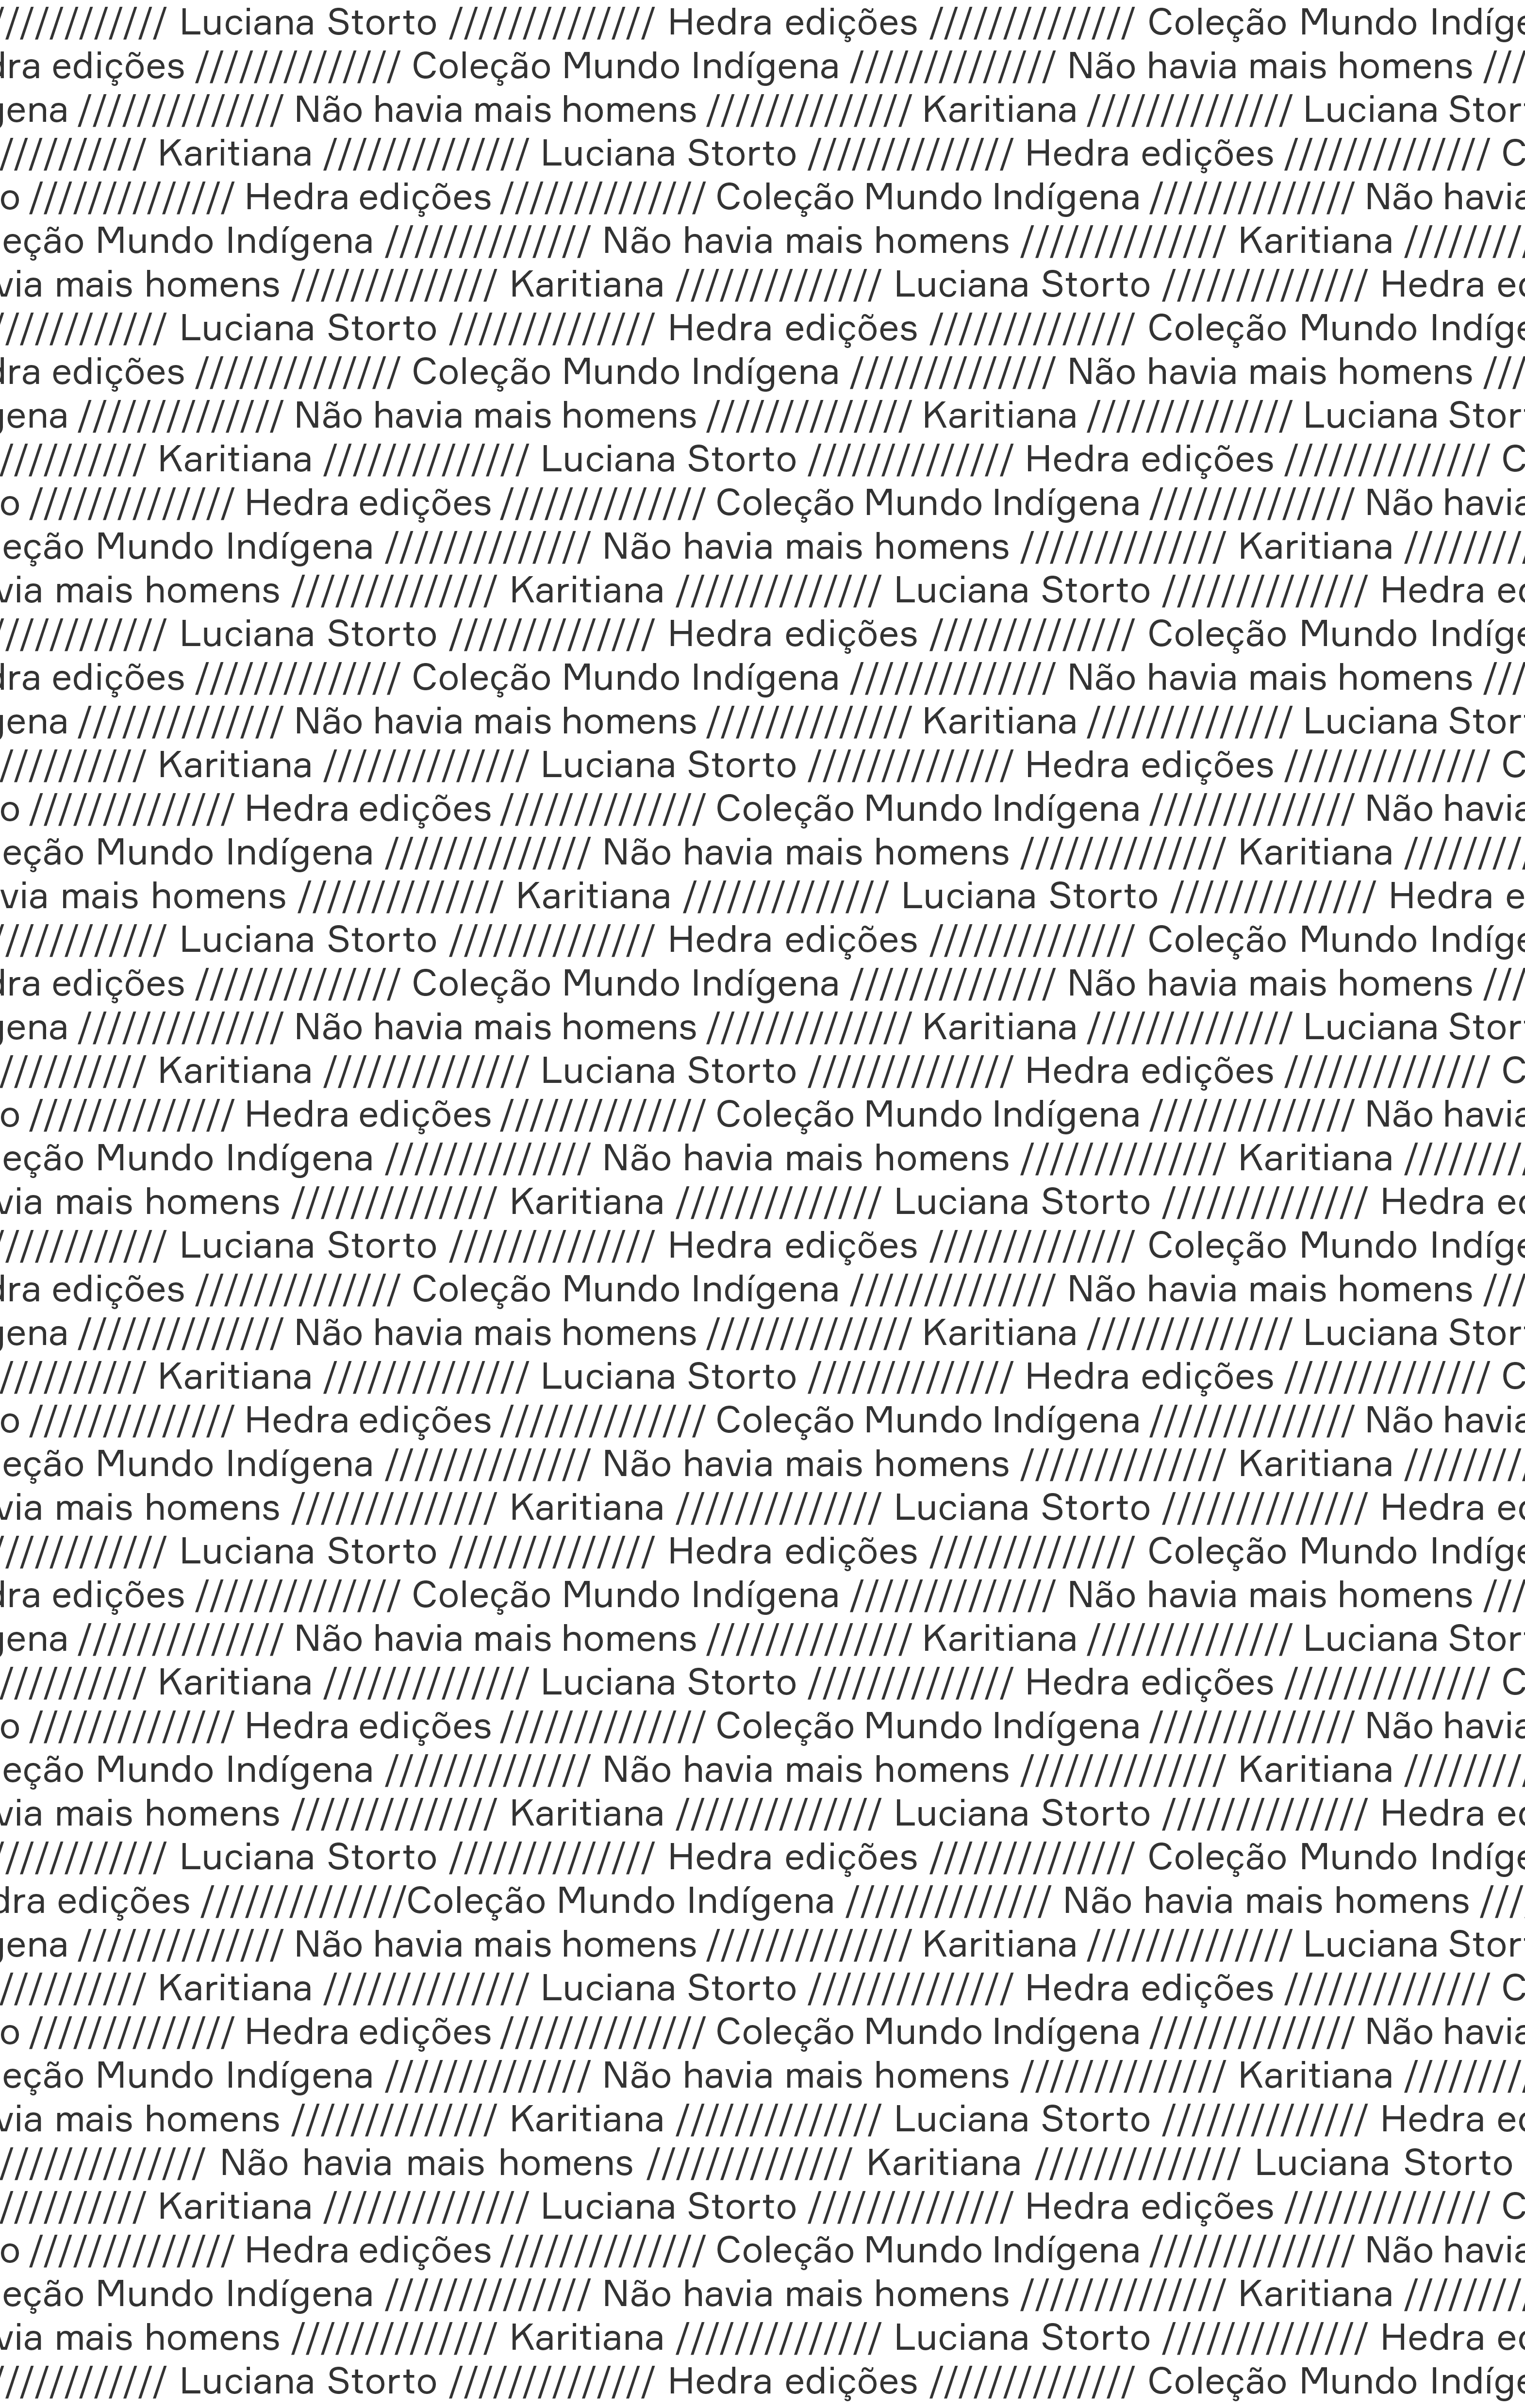
\includegraphics[width=138mm]{./MI_STORTO_HOMENS_ABERTURA.png}  
\end{textblock*}
\clearpage
\pagebreak

\thispagestyle{empty}
\begin{textblock*}{2.625in}(0pt,0pt)%
\vspace*{-2.4cm}
\hspace*{-2.3cm}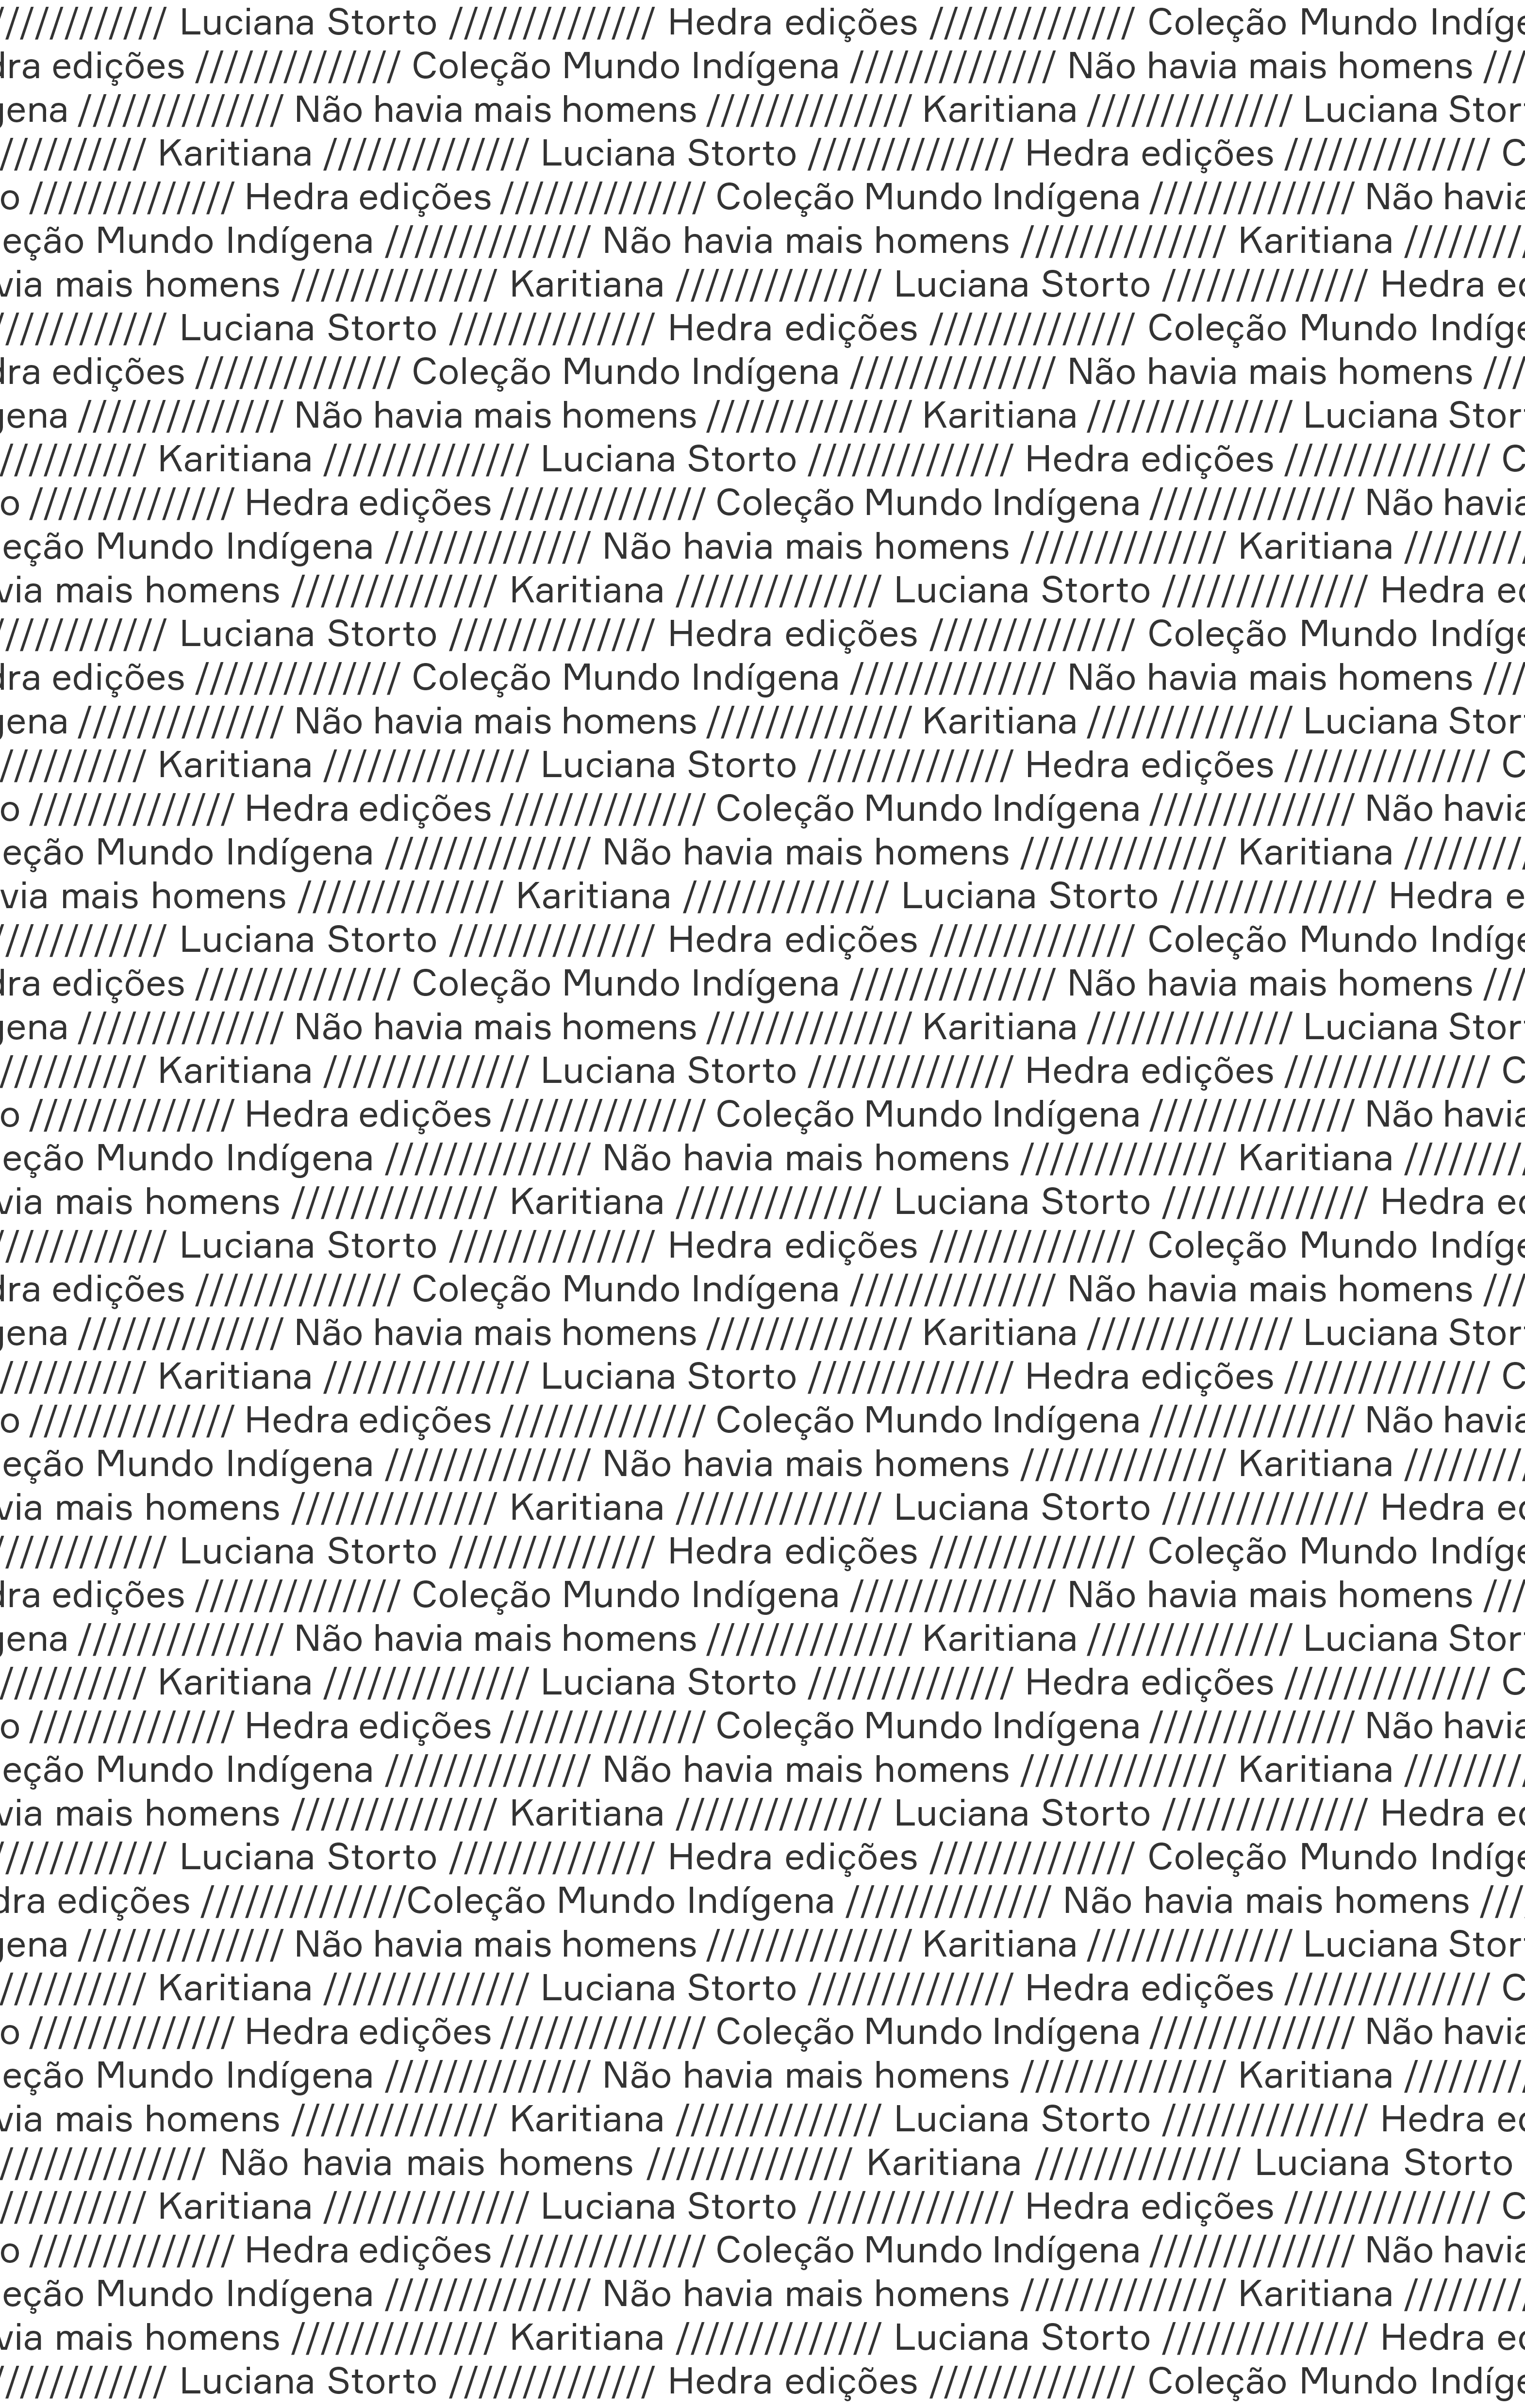
\includegraphics[width=138mm]{./MI_STORTO_HOMENS_ABERTURA.png}  
\end{textblock*}
\clearpage

\thispagestyle{empty}

% Tamanhos
% \tiny
% \scriptsize
% \footnotesize
% \small 
% \normalsize
% \large 
% \Large 
% \LARGE 
% \huge
% \Huge

% Posicionamento
% \centering 
% \raggedright
% \raggedleft
% \vfill 
% \hfill 
% \vspace{Xcm}   % Colocar * caso esteja no começo de uma página. Ex: \vspace*{...}
% \hspace{Xcm}

% Estilo de página
% \thispagestyle{<<nosso>>}
% \thispagestyle{empty}
% \thispagestyle{plain}  (só número, sem cabeço)
% https://www.overleaf.com/learn/latex/Headers_and_footers

% Compilador que permite usar fonte de sistema: xelatex, lualatex
% Compilador que não permite usar fonte de sistema: latex, pdflatex

% Definindo fontes
% \setmainfont{Times New Roman}  % Todo o texto
% \newfontfamily\avenir{Avenir}  % Contexto

\begingroup\thispagestyle{empty}\vspace*{.05\textheight} 

              {\formular
              \huge
              \noindent
              \textbf{Não havia mais homens}\\ 
              
              \vspace{-0.5cm}
              
              \noindent{}{\LARGE Imbodn oko taso}}

              %\vspace{0.5cm}

              %\noindent{}\textit{Ou o livro das transformações, contadas\\pelos Yanomami do  grupo Parahiteri}
                    
\endgroup
\vfill
\pagebreak       % [Frontistício]
%\newcommand{\linhalayout}[2]{{\tiny\textbf{#1}\quad#2\par}}
\newcommand{\linha}[2]{\ifdef{#2}{\linhalayout{#1}{#2}}{}}

\begingroup\tiny
\parindent=0cm
\thispagestyle{empty}

\textbf{edição brasileira©}\quad			 {Hedra \the\year}\\
\textbf{organização e tradução©}\quad		 {Luciana Storto}\\
\textbf{coorganização}\quad			 	 	 {Íris Morais Araújo e Karin Vivanco}\\
%\textbf{tradução}\quad			 			 {Izaque João}\\
%\textbf{posfácio©}\quad			 		 {Fábio Zuker}\\
%\textbf{ilustração©}\quad			 		 {copyrightilustracao}\medskip

%\textbf{edição consultada}\quad			 {edicaoconsultada}\\
%\textbf{primeira edição}\quad			 	 {Acontecimentos}\\
%\textbf{agradecimentos}\quad			 	 {agradecimentos}\\
%\textbf{indicação}\quad			 		 {indicacao}\medskip

\textbf{coordenação da coleção}\quad		 {Luísa Valentini}\\
\textbf{edição}\quad			 			 {Jorge Sallum}\\
\textbf{coedição}\quad			 			 {Suzana Salama}\\
\textbf{assistência editorial}\quad			 {Paulo Henrique Pompermaier}\\
\textbf{capa}\quad			 				 {Lucas Kroëff}\\
%\textbf{iconografia}\quad			 		 {iconografia}\\
%\textbf{imagem da capa}\quad			 	 {imagemcapa}\medskip

\textbf{\textsc{isbn}}\quad			 		 {978-65-89705-77-2}

\hspace{-5pt}\begin{tabular}{ll}
\textbf{conselho editorial} & Adriano Scatolin,  \\
							& Antonio Valverde,  \\
							& Caio Gagliardi,    \\
							& Jorge Sallum,      \\
							& Ricardo Valle,     \\
							& Tales Ab'Saber,    \\
							& Tâmis Parron      
\end{tabular}
 
\bigskip
\textit{Grafia atualizada segundo o Acordo Ortográfico da Língua\\
Portuguesa de 1990, em vigor no Brasil desde 2009.}\\

\vfill
\textit{Direitos reservados em língua\\ 
portuguesa somente para o Brasil}\\

\textsc{editora hedra ltda.}\\
R.~Fradique Coutinho, 1139 (subsolo)\\
05416--011 São Paulo \textsc{sp} Brasil\\
Telefone/Fax +55 11 3097 8304\\\smallskip
editora@hedra.com.br\\
www.hedra.com.br\\

Foi feito o depósito legal.

\endgroup
\pagebreak     % [Créditos]
% Tamanhos
% \tiny
% \scriptsize
% \footnotesize
% \small 
% \normalsize
% \large 
% \Large 
% \LARGE 
% \huge
% \Huge

% Posicionamento
% \centering 
% \raggedright
% \raggedleft
% \vfill 
% \hfill 
% \vspace{Xcm}   % Colocar * caso esteja no começo de uma página. Ex: \vspace*{...}
% \hspace{Xcm}

% Estilo de página
% \thispagestyle{<<nosso>>}
% \thispagestyle{empty}
% \thispagestyle{plain}  (só número, sem cabeço)
% https://www.overleaf.com/learn/latex/Headers_and_footers

% Compilador que permite usar fonte de sistema: xelatex, lualatex
% Compilador que não permite usar fonte de sistema: latex, pdflatex

% Definindo fontes
% \setmainfont{Times New Roman}  % Todo o texto
% \newfontfamily\avenir{Avenir}  % Contexto

\begingroup\thispagestyle{empty}\vspace*{.05\textheight} 

              \formular
              \huge
              \noindent
              \textbf{Não havia mais homens}

              \bigskip  
              
              \large
              \noindent
              \textit{Imbodn oko taso}
              \vspace{12.5em}
              
              \newfontfamily\garamond{EBGaramond12-Regular}
              {\selectfont\garamond\small\noindent Luciana Storto (\textit{organização e tradução})}

              \bigskip

              \noindent
              {\selectfont\garamond\small\noindent 1ª edição}

              \vfill

              \newfontfamily\timesnewroman{Times New Roman}
              {\noindent\fontsize{30}{40}\selectfont \timesnewroman hedra}

              \noindent{\selectfont\garamond\small
              \noindent São Paulo \quad\the\year}


\endgroup
\pagebreak
	       % [folha de rosto]
% nothing			is level -3
% \book				is level -2
% \part				is level -1
% \chapter 			is level 0
% \section 			is level 1
% \subsection 		is level 2
% \subsubsection 	is level 3
% \paragraph 		is level 4
% \subparagraph 	is level 5
\setcounter{secnumdepth}{-3}
\setcounter{tocdepth}{0}

% \renewcommand{\contentsname}{Índex} 	% Trocar nome do sumário para 'Índex'
%\ifodd\thepage\relax\else\blankpage\fi 	% Verifica se página é par e coloca página branca
%\tableofcontents*

\pagebreak
\begingroup \footnotesize \parindent0pt \parskip 5pt \thispagestyle{empty} \vspace*{-0.5\textheight}\mbox{} \vfill
\baselineskip=.92\baselineskip
\textbf{Não havia mais homens} contém quatro narrativas de tradição oral dos Karitiana, contadas na primeira parte da década de 1990 por três narradores que são reconhecidas lideranças do grupo, conhecedores da mitologia e história do povo. Os mitos do sol e da lua foram contados pelo cacique Garcia, o ritual de iniciação masculino \textit{Osiip} por Cizino, que é o último pajé Karitiana, e a narrativa final, que retrata o reencontro ente as duas últimas aldeias da etnia, de onde foi tirado o título do livro \textit{Não havia mais homens}, foi contada por Barabadá. As narrativas foram gravadas pela organizadora, e depois transcritas e traduzidas com a ajuda de falantes da língua. Elas registram mitos e eventos importantes para o povo e devem ser lidos como parte de sua literatura. 

\textbf{Luciana Storto} é doutora em Linguística pelo Massachusetts Institute of
Technology e professora do Departamento de Linguística da Universidade
de São Paulo (\textsc{usp}). Estuda a língua karitiana desde 1992.

% \textbf{Íris Morais Araújo} é doutora em Antropologia Social pela Universidade de
% São Paulo e pesquisadora do Centro de Pesquisa em Etnologia Indígena da
% Universidade Estadual de Campinas.

% \textbf{Karin Vivanco} é doutora em Linguística pela Universidade de São Paulo,
% foi bolsista de pós-doutorado do Departamento de Linguística da
% Universidade Estadual de Campinas e atualmente
% é professora da \textsc{ufrgs}.

\textbf{Coleção Mundo Indígena} reúne materiais produzidos com pensadores de diferentes povos indígenas e pessoas que pesquisam, trabalham ou lutam pela garantia de seus direitos. Os livros foram feitos para serem utilizados pelas comunidades envolvidas na sua produção, e por isso uma parte significativa das obras é bilíngue. Esperamos divulgar a imensa diversidade linguística dos povos indígenas no Brasil, que compreende mais de 150 línguas pertencentes a mais de trinta famílias linguísticas.

%(\textsc{fapesp} nº 2019/11661-4)

\endgroup

\pagebreak\thispagestyle{empty}\movetooddpage
{\begingroup\mbox{}\pagestyle{empty}
\pagestyle{empty} 
% \renewcommand{\contentsname}{Índex} 	% Trocar nome do sumário para 'Índex'
%\ifodd\thepage\relax\else\blankpage\fi 	% Verifica se página é par e coloca página branca
\addtocontents{toc}{\protect\thispagestyle{empty}}
\tableofcontents*\clearpage\endgroup}

\chapter{Nota da organizadora}

\noindent{}Os Karitiana são um grupo indígena ainda pouco conhecido no Brasil. Vivem no atual estado de Rondônia, considerado o lugar de origem da língua-mãe de todas as línguas tupi. Falam a língua de mesmo nome, que é a única remanescente da família linguística arikém, o que lhes confere uma importância central para os estudos comparativos das línguas tupi e, consequentemente, das línguas indígenas como um todo.

\textls[-10]{Aproximaram-se dos não indígenas durante o ciclo da borracha. Tanto a memória do grupo quanto os documentos não indígenas dão destaque para esses vínculos de trabalho caracterizados pela violência dos patrões. Nesse período, os não indígenas disseminaram entre eles diversas doenças, como a gripe e o sarampo. Por isso, em meados do século \textsc{xx}, os Karitiana sofreram um grande declínio populacional chegando a apenas 64 pessoas na década de 1970. Para que continuassem a existir, dois grupos locais decidiram viver juntos, casando-se entre si, e procuraram o Serviço de Proteção aos Índios, para que seus direitos como povo indígena fossem garantidos. No censo realizado pelo linguista Ivan Rocha em 2017, os Karitiana contavam com 397 pessoas.}

Atualmente, eles habitam sete aldeias, sendo cinco na Terra Indígena Karitiana, demarcada em 1986, e duas fora dela, em áreas que são parte do seu território tradicional. Algumas famílias também moram nas cidades rondonienses de Porto Velho, a capital, e em Cacoal. Além de trabalharem em atividades agrícolas, no manejo dos recursos florestais e na produção de artesanato, os Karitiana também são profissionais das áreas de saúde e educação. O grupo luta historicamente pela garantia de seus direitos, como a ampliação da terra indígena e o fortalecimento da educação e da saúde indígena.

\chapter{Como foi feito este livro}

\begin{flushright}
\textsc{íris morais araújo}\\
\textsc{karin vivanco}
\end{flushright}

\noindent{}Em 1992, a linguista Luciana Storto
iniciou sua pesquisa sobre a língua karitiana. Para poder estudar o
idioma, ela gravou, neste e nos cinco anos seguintes, histórias
tradicionais do povo Karitiana --- mitos de origem, rituais e narrativas
históricas. As histórias foram narradas por Pereira Karitiana, Barabadá
Karitiana, Garcia Karitiana, Antonio Paulo Karitiana, Cizino Karitiana,
Joana Karitiana e Nazaré Karitiana, alguns dos homens e mulheres mais
velhos de então, tidos como conhecedores da arte verbal. Com o
importante apoio de interlocutores indígenas mais jovens, os atuais
professores Nelson Karitiana, João Karitiana, Luiz Karitiana e Inácio
Karitiana, bem como de vários outros falantes da língua, foram feitas as
primeiras transcrições e traduções do material.

Os linguistas trabalham transcrevendo e traduzindo as narrativas
sentença a sentença. A passagem da fala para a escrita é o primeiro
desafio colocado, já que em qualquer língua existem diferenças entre
como se fala e como se escreve. Para chegar à escrita da fala, a maneira
escolhida pela linguista foi ouvir cada sentença conjuntamente com os
jovens karitiana com os quais trabalhou na transcrição e tradução,
pausar o áudio, e ir decidindo o que permaneceria no texto transcrito e
o que seria deixado de fora da transcrição. Este foi um modo de manter o
conteúdo da narrativa e sua estrutura prosódica e artística, sem incluir
os erros, hesitações e repetições não intencionais, naturais da fala
ocorridas enquanto o falante busca na memória pelo próximo assunto a ser
narrado.

Neste livro, as frases numeradas incluíram mais de uma sentença quando
foram pronunciadas com uma única entoação. Os linguistas fazem esses
registros com muitos detalhes. Para eles, é importante saber como
funciona cada parte de uma única palavra, chamada de \textit{morfema}, e
cada palavra em uma frase. Para que essas informações estejam
disponíveis para outros estudiosos, as sentenças são registradas em três
linhas: 

\begin{enumerate}
\item A linha do original na língua indígena, com um hífen
separando cada morfema dentro das palavras\footnote{\textit{I-a-oky padni Gokyp}.}

\item A linha chamada
\textit{glosa}, na qual se faz uma tradução para o português do
significado de cada morfema\footnote{\textit{Terceira pessoa-passiva-morrer não Sol}.}

\item A linha contendo uma tradução
aproximada da sentença inteira para o português; neste caso, o linguista
por vezes precisa fazer escolhas entre uma tradução literal da sentença
e uma tradução mais natural\footnote{\textit{Não se mata o sol/\,O Sol não pode ser morto}.}

\end{enumerate}

As transcrições apresentadas neste livro foram editadas para uma leitura
confortável, mas se buscou preservar certas características da narrativa
oral, como a repetição poética (repetição da sentença anterior com uma
modificação, a fim de criar um efeito poético na forma ou no
significado) e estruturas sintáticas comuns na língua karitiana: um
exemplo são as inversões na ordem de palavras.\footnote{Por exemplo, \textit{Caça, o
Osiip desnorteia} em vez de \textit{O Osiip desnorteia a caça.}}

\section{quem participou}

\paragraph{Barabadá Karitiana} foi um pajé Karitiana pertencente ao grupo Joari
 (também conhecido como Capivari). Ele narrou o encontro, vivenciado por
 ele, entre dois grupos de Karitiana que viviam em aldeias separadas, os
 Joari (ou Capivari) e os Karitiana. Estes grupos passaram a viver juntos
 na Terra Indígena Karitiana.

 \paragraph{Cizino Karitiana} é o atual pajé e cacique Karitiana. Ele narrou o ritual
 de iniciação masculina, intitulado \textit{Osiip}, pelo qual passou várias
 vezes.

 \paragraph{Garcia Karitiana} foi um cacique Karitiana. Ele narrou os mitos de origem
 do sol e da lua.

 \paragraph{Inácio Karitiana} é licenciado em Educação Básica Intercultural pela
 Universidade Federal de Rondônia e professor da Escola Indígena Estadual
 de Ensino Fundamental Kity Pypydnipa.

 \paragraph{Ivan Rocha} é doutor em Linguística pela Universidade de São Paulo e
 pesquisador visitante do Museu Paraense Emílio Goeldi, com bolsa do
 Programa de Capacitação Institucional (\textsc{pci}) do Ministério da Ciência,
 Tecnologia e Inovação (\textsc{mcti}/\textsc{cnp}q).

 \paragraph{João Karitiana} é licenciado em Educação Básica Intercultural pela
 Universidade Federal de Rondônia e professor da Escola Indígena Estadual
 de Ensino Fundamental e Médio Kyõwã.

 \paragraph{Luiz Karitiana} é licenciado em Educação Básica Intercultural pela
 Universidade Federal de Rondônia e professor da Escola Indígena Estadual
 de Ensino Fundamental e Médio Kyõwã.

 \paragraph{Nelson Karitiana} é licenciado em Educação Básica Intercultural pela
 Universidade Federal de Rondônia e professor da Escola Indígena Estadual
 de Ensino Fundamental e Médio Kyõwã.

 \paragraph{Valdomiro Karitiana} é filho de Barabadá Karitiana. Ele acompanhou a
 linguista durante a gravação da história do encontro entre os dois
 grupos locais e auxiliou na transcrição e tradução.

% Nem todas as narrativas gravadas por Luciana na década de 1990 chegaram
% a ser transcritas e traduzidas, mas todas as que o foram e que não fazem
% parte deste volume serão publicadas futuramente em outro volume desta
% coleção.

\chapter[Para ler as palavras karitiana]{Para ler as palavras\break karitiana}

\textls[-10]{Neste livro, foi adotada a ortografia elaborada pela linguista Luciana Storto, que coordenou um programa de alfabetização da língua karitiana desenvolvido junto à comunidade na década de 1990 e aprovado por ela em 1996, quando as convenções ortográficas foram registradas no material de apoio ao aprendizado da ortografia karitiana, que tem sido usado desde então no ensino de sua língua materna. Atualmente, o grupo vem discutindo a reformulação de algumas dessas convenções ortográficas.}

\section{Vogais}

\begingroup
\begin{tabular}{rl}
/a/ & como \textit{a} em \textit{até}\\
/e/ & como \textit{e} em \textit{mesa}\\
/i/ & como \textit{i} em \textit{idoso}\\
/o/ & como \textit{o} em \textit{hoje}\\
/y/ & como um som intermediário entre \textit{i} e \textit{u}\protect\footnotemark\\
\end{tabular}

\footnotetext{\textls[-10]{Esse som não possui um equivalente no português do Brasil. Para pronunciá-lo, se pode falar um \textit{i} e, gradualmente, mover a língua em direção a um \textit{u}. Quando a língua estiver em uma posição entre \textit{i} e \textit{u}, esta será a pronúncia do \textit{y}. Os linguistas classificam esse som como uma vogal ``central alta'' e, a partir de um inventário internacional convencional de símbolos, o Alfabeto Fonético Internacional, transcrevem-no como um ``i'' tachado, o símbolo ``ɨ''.}}
\endgroup

\section{Consoantes}

\begingroup
\begin{tabular}{rl}
/b/ & como \textit{b} em \textit{boto}\\
/d/ & como \textit{d} em \textit{dedo}\\
/g/ & como \textit{g} em \textit{gato}\\
/h/ & como \textit{r} em \textit{rato}\\
/j/ & como \textit{dj} no início da palavra; no meio \textit{i} como em \textit{saia}\\
/k/ & como \textit{c} em \textit{casa}\\
/m/ & como \textit{m} em \textit{mulher}\\
/n/ & como \textit{n} em \textit{nariz}\\
/p/ & como \textit{p} em \textit{pé}\\
/r/ & como \textit{r} em \textit{arara}\\
/s/ & como \textit{s} em \textit{sapo}\\
/t/ & como \textit{t} em \textit{tatu}\\
/w/ & como \textit{u} em \textit{água}\\
/x/ & como \textit{tch} em \textit{tchau}\\
/`/ & \textls[-15]{uma pausa, como quando dizemos \textit{ã--ã} com o sentido de \textit{não}}\protect\footnotemark
\end{tabular}\\

\footnotetext{\textls[10]{Corresponde a uma breve pausa entre as duas sílabas, que equivale a uma obstrução, na região das cordas vocais, do fluxo de ar que vem do pulmão, chamada de consoante oclusiva glotal no alfabeto fonético.}} 
\endgroup
\part[Não havia mais homens]{Não havia mais\break homens}

\chapter*{}
\thispagestyle{empty}

\vspace*{\fill}
\paragraph{A história de Gokyp, o Sol} A história do Sol é uma das narrativas que compõem o repertório de mitos dos Karitiana. Nascido como uma criança muito quente, que parecia febril, ninguém conseguia chegar muito perto do Sol sem se queimar. As
pessoas, preocupadas com o perigo que ele significava para a comunidade,
pensaram em matá-lo. Cada vez mais quente, o Sol subiu pelo esteio de
uma casa e decidiu ir para o céu, onde vive até hoje.\footnote{A narrativa aqui publicada foi contada por Garcia Karitiana para Luciana Storto, que a transcreveu e traduziu com Nelson Karitiana. Para esta
publicação, o material foi editado por Íris Morais Araújo e Karin
Vivanco. Uma primeira transcrição, glosagem e tradução desta narrativa foi publicada por Storto na \textit{Revista Linguíʃtica} 15 (2019).}
\vspace*{\fill}

\chapter{O Sol}

\begin{linenumbers}
%\begin{enumerate}
%\item 
\noindent Dizem que o Sol vivia antigamente\\
%\item \\
Dizem que o Sol começou sua existência como uma criança\\
%\item \\
Dizem que o Sol vivia
\end{linenumbers}

\bigskip

\begin{linenumbers}
%\item 
\noindent Então os homens disseram \textit{O que é isso?}\\
%\item \\
Dizem que a vida começou como uma doença para ele\\
%\item \\
Dizem que a criança ficava cada vez mais quente
\end{linenumbers}

\bigskip

\begin{linenumbers}
%\item 
\noindent \textit{Esse aí está doente?}, falava o seu pessoal\\
%\item \\
Seria semelhante a uma doença\\
%\item \\
Mas ele não estava doente realmente\\
%\item \\
Ele nunca esteve doente
\end{linenumbers}

\bigskip

\begin{linenumbers}
%\item 
\noindent Então dizem que o calor dele ficava cada vez mais intenso\\
%\item \\
O Sol era meio quente e foi ficando mais quente\\
%\item \\
Naquele momento, ele se tornaria o Sol
\end{linenumbers}

\bigskip

\begin{linenumbers}
%\item 
\noindent Então aconteceu\\
%\item \\
\textit{Ah, o que é isso?}, diziam os homens\\
%\item \\
Aí, ele não existia mais\\
%\item \\
Então ele se tornou tão grande que não podia mais viver aqui\\
%\item \\
Ele se tornou enorme
\end{linenumbers}

\bigskip

\begin{linenumbers}
%\item 
\noindent Aí, dizem que o Sol não queimava mais só um pouco\\
%\item 
Dizem que ele se tornou incandescente\\
%\item 
Quando sua incandescência ficou insustentável, dizem que os homens
queriam matá-lo\\
%\item 
Porque ele não era mais um ser humano
\end{linenumbers}

\bigskip

\begin{linenumbers}
%\item 
\noindent Os homens tinham um desejo de matar\\
%\item 
Então não o fariam\\
%\item 
Aí, os homens pensaram\\
%\item 
\textit{O Sol não pode ser morto}
\end{linenumbers}

\bigskip

\begin{linenumbers}
%\item 
\noindent Eles pensaram que era assim que fariam\\
%\item 
Eles pensavam que ele era humano\\
%\item 
Mas ele estava ficando diferente, meio fraco
\end{linenumbers}

\bigskip

\begin{linenumbers}
%\item 
\noindent Por causa disso, os homens sentiam vontade de matá-lo\\
%\item 
Matá-lo é o que queriam fazer\\
%\item 
Aí, ele continuou a viver
\end{linenumbers}

\bigskip

\begin{linenumbers}
%\item 
\noindent Dizem que ele saiu pelo esteio central do telhado da casa\\
%\item 
Porque dizem que os homens tinham o desejo de matá-lo\\
%\item 
Sabia-se que queriam matá-lo
\end{linenumbers}

\bigskip

\begin{linenumbers}
%\item 
\noindent Na frente deles, então, ele saiu\\
%\item \\
Pelo esteio central da casa ele sairia\\
%\item \\
Aí, vieram os homens com bordunas para matá-lo, sorrateiramente\\
%\item \\
Mas eles não podiam mais se aproximar dele\\
%\item 
Ele estava muito incandescente mesmo
\end{linenumbers}

\bigskip

\begin{linenumbers}
%\item 
\noindent Foi então que, dizem, ele saiu pelo esteio central da casa\\
%\item \\
Aí, o Sol cantou antes de sair\\
%\item \\
\textit{Tragam-me para dentro, mulheres}\\
%\item \\
\textit{Tragam-me para dentro, mulheres}\\
%\item \\
\textit{Tragam-me para dentro, tragam-me para dentro, mulheres}\\
%\item \\
\textit{Pois o crânio partido está me matando}\\
%\item \\
Assim disse o Sol enquanto ele subia\\
%\item \\
Então dizem que o Sol subiu; \textit{Pro alto} ele foi\\
%\item \\
Então dizem que quem queria matá-lo morreu enquanto ele estava subindo\\
%\item 
\textit{Caíram esparramados}, os homens
\end{linenumbers}

\bigskip

\begin{linenumbers}
%\item 
\noindent O Sol subiu para as alturas\\
%\item \\
Então o Sol ficou incandescente, incandescente de verdade\\
%\item \\
Assim, dizem, é que a história do Sol deve ser contada
%\end{enumerate}
\end{linenumbers}

\chapter{Gokyp}

%\begin{enumerate}
%\item 
\begin{linenumbers}
\noindent Pyry'a sarytyn keerep Gokyp\\
%\item \\
Õwã horot taka'oot saryt Gokyp\\
%\item 
Taaka andyk saryt Gokyp
\end{linenumbers}

\bigskip

\begin{linenumbers}
%\item 
\noindent Masõng \textit{ti'a hỹ?}, iri'aj taso\\
%\item \\
Kinda oti horot taka'oot saryt ihot iaka\\
%\item 
Okywyra okywyra okywyra taaka saryt õwã
\end{linenumbers}

\bigskip
%\item 
\begin{linenumbers}

\noindent \textit{A kinda otidna hỹ?}, iri'a andyki ijiriso\\
%\item \\
Kinda oti horot iakaj\\
%\item \\
Ikinda otidni\\
%\item 
Takinda otidna sogng iaki
\end{linenumbers}

\bigskip

\begin{linenumbers}
%\item 
\noindent Masong naakat okyp okyp ywytiyty tat, iri'aj\\
%\item \\
Ty'in taakat iokyp pywytiyri Gokyp\\
%\item 
Gokyp pasagngam iakabman
\end{linenumbers}

\bigskip

\begin{linenumbers}
%\item 
\noindent Masong naka'a andyk\\
%\item \\
\textit{Ãh ti'a tyka hỹ?}, iri'aj taso\\
%\item \\
Masong imbodnoko\\
%\item \\
Atykiri iaka padnoko hak tatyyt tykiri\\
%\item 
Tyyty tat, iri'aj
\end{linenumbers}

\bigskip

\begin{linenumbers}
%\item 
\noindent Atykiri ipikyp owogoko saryty padni Gokyp\\
%\item \\
Napikybm saryt\\
%\item \\
I pikywyt tykiri, iatakipawyt tykiri napyting saryt iokyty taso\\
%\item 
Masong iaki padnoko
\end{linenumbers}

\bigskip

\begin{linenumbers}
%\item 
\noindent Napymbowak ity taso\\
%\item \\
Masong iaoky padnaty\\
%\item \\
Masong nakakãrãt taso\\
%\item 
Iaoky padni Gokyp
\end{linenumbers}

\bigskip

\begin{linenumbers}
%\item 
\noindent Masong kahyt i'at, irikãraj͂\\
%\item \\
Yjxa pitat i'at tykat, irikãrãj\\
%\item 
Myn hodno yjsararaj sat iakiip
\end{linenumbers}

\bigskip

\begin{linenumbers}
%\item 
\noindent Masong napymbowak saryt ity taso\\
%\item \\
Iokyty napyting\\
%\item 
Masong ta'a tyka siit
\end{linenumbers}

\bigskip

\begin{linenumbers}
%\item 
\noindent Namboryt saryt ambiity sopakat\\
%\item \\
Masong napymbowak saryt it taso\\
%\item 
Ta'ãty ipymbowak tyso
\end{linenumbers}

\bigskip

\begin{linenumbers}
%\item 
\noindent Asonderep masong namboryt\\
%\item \\
Ambi sopakat imboryri\\
%\item \\
Masong naymbykyjy'oom taso iokyp meresõ tyyt\\
%\item \\
Ipynotam padnoko I\\
%\item 
Piikyp piikyp harara I
\end{linenumbers}

\bigskip

\begin{linenumbers}
%\item 
\noindent Masong namboryt saryt i ambi sopakat\\
%\item \\
Masong nakahyryj͂a tatat tysypy'oot Gokyp\\
%\item \\
\textit{Ajymymewã j͂onso}\\
%\item \\
\textit{Ajymymewã j͂onso}\\
%\item \\
\textit{Ajymymewã ymymewã j͂onso}\\
%\item \\
\textit{Opa pyka yoky tyki}\\
%\item \\
Masong naka'a saryt Gokyp taambo tyki'oot\\
%\item \\
Masong naambo saryt Gokyp; atoop iri'aj hoop\\
%\item \\
Masong ta'ãty ipymbowak atapopi saryt tatat tysypy'oot\\
%\item 
\textit{Syyryp} iri'aj taso
\end{linenumbers}

\bigskip

\begin{linenumbers}
%\item 
\noindent Naambot ohyn Gokyp\\
%\item \\
Masong naakat piikyp piikyp harara Gokyp\\
%\item 
Naka'a saryt kahyt Gokyp pynhadna
%\end{enumerate}
\end{linenumbers}


\chapter*{}
\thispagestyle{empty}

\vspace*{\fill}
\paragraph{A história do Lua, Oti} A história do Lua, um homem chamado Oti, é uma importante narrativa que também compõe o \textit{corpus} mítico dos Karitiana. Quando vivia entre
os humanos, Oti teve relações sexuais não consentidas com a mãe e a
irmã. Esta última descobriu que o irmão a visitava à noite, no escuro,
após seguir a sugestão de seu namorado de passar tinta de jenipapo no
intruso durante uma dessas relações sexuais. A mãe, por sua vez, foi
forçada por Lua a ceder a seus desejos quando foram para a floresta
buscar os frutos da palmeira patauá.\footnote{\textit{Oenocarpus bataua}, também 
conhecida por \textit{patuá} ou \textit{patoá}.} Após esses eventos, Lua subiu
nessa palmeira e foi viver no céu. Contudo, antes disso, cortou suas
próprias pernas, para que fossem sepultadas junto com seus objetos e
decidiu que todas as mulheres, a partir de então, passariam a menstruar.\footnote{A narrativa de Oti foi contada por Garcia Karitiana para Luciana Storto,
que a transcreveu e fez uma tradução preliminar. Para esta publicação, o
material foi traduzido e revisado por Inácio Karitiana, Nelson
Karitiana, Íris Morais Araújo, Karin Vivanco e Luciana Storto.}
\vspace*{\fill}


\chapter{O Lua}

%\begin{enumerate}
%\item 
\begin{linenumbers}
\noindent Assim, dizem, é que fez o Lua\\
%\item \\
O Lua vivia\\
%\item \\
O Lua era homem, também\\
%\item 
Homem adulto
\end{linenumbers}

\bigskip

\begin{linenumbers}
%\item 
\noindent Então dizem que o Lua ainda vivia entre nós\\
%\item \\
Ainda estava vivo\\
%\item \\
Dizem que o Lua transou com sua irmã menor\\
%\item \\
Aí, ela pensou que ele era seu namorado\\
%\item 
E ela permitiu que o Lua transasse com ela, a irmã do Lua
\end{linenumbers}

\bigskip

\begin{linenumbers}
%\item 
\noindent Então dizem que o namorado dela mexeu com ela\\
%\item \\
Transou com ela\\
%\item \\
\textit{Ah! Quem será?}\\
%\item \\
Ela disse assim\\
%\item \\
Aí, o namorado veio na direção dela\\
%\item \\
\textit{Vem}, disse o namorado dela\\
%\item 
\textit{Você veio de novo?}, ela disse
\end{linenumbers}

\bigskip

\begin{linenumbers}
%\item 
\noindent Ah! O seu namorado falou: \textit{O que é isso?}\\
%\item \\
\textit{Ah! Não era você que veio antes?}, ela disse\\
%\item \\
\textit{Eu ainda não vim com você}. \textit{Por quê?}, disse\\
%\item \\
\textit{Ele mexeu várias vezes comigo. Quantas vezes você já veio aqui comigo?}\\
%\item \\
\textit{Só agora mesmo eu vim aqui com você}\\
%\item 
Disse o namorado dela
\end{linenumbers}

\bigskip

\begin{linenumbers}
%\item 
\noindent \textit{Não é você que vem transando comigo?}\\
%\item \\
\textit{Qual homem será?}\\
%\item \\
\textit{Qual homem será que vem transando comigo?}\\
%\item \\
\textit{Ah!}, falou o namorado\\
%\item \\
\textit{Eu achei que fosse você}, disse a irmã do Lua\\
%\item 
Então foi assim
\end{linenumbers}

\bigskip

\begin{linenumbers}
%\item 
\noindent Aí o namorado disse \textit{Hum\ldots{}}\\
%\item \\
\textit{Passa jenipapo no corpo dele}, o namorado falou\\
%\item \\
\textit{Você vai passar jenipapo amanhã}\\
%\item \\
\textit{Amanhã você passa jenipapo no rosto dele e depois disso você vai\\
%\item \\
rosto dele}\\
%\item \\
\textit{Você olha o rosto de todos os homens}\\
%\item \\
\textit{Então você vai ver}\\
%\item \\
\textit{É você mesmo?}\\
%\item \\
\textit{Então você vai falar}\\
%\item \\
\textit{Quando você souber, você vai falar assim}\\
%\item \\
Então ela nunca pensou que seria seu irmão\\
%\item \\
\textit{Hã}, disse\\
%\item \\
\textit{Você passa jenipapo sorrateiramente em você}, disse\\
%\item \\
\textit{Você vai esconder o jenipapo embaixo da rede}, disse\\
%\item \\
\textit{Você vai deixar o jenipapo embaixo para quando ele vier}\\
%\item \\
\textit{Hoje ele vem de novo}\\
%\item \\
\textit{Ele não demora a vir de novo}\\
%\item 
\textit{Você não vai se atrapalhar}
\end{linenumbers}

\bigskip

\begin{linenumbers}
%\item 
\noindent Então ela ficou preparada\\
%\item \\
Ela se preparou para a chegada dele\\
%\item \\
Passou jenipapo nela, ficou preta\\
%\item \\
Aí sobrou\\
%\item \\
Então dormiu\\
%\item \\
A mulher dormiu com todos enfeites e pinturas\\
%\item 
A mulher estava bonita
\end{linenumbers}

\bigskip

\begin{linenumbers}
%\item 
\noindent Então no mesmo dia o Lua, o irmão dela, chegou de novo\\
%\item \\
Era o irmão dela\\
%\item \\
Ela não sabia\\
%\item \\
Dizem que o Lua transava com a irmã. Ela foi a primeira filha da mãe dele, foi a primeira dela\\
%\item 
Então foi dormir
\end{linenumbers}

\bigskip

\begin{linenumbers}
%\item 
\noindent Aí, escureceu o dia\\
%\item \\
Antes de escurecer, ele viria\\
%\item \\
Veio\\
%\item \\
Então ela empurrou o jenipapo embaixo da rede dela\\
%\item \\
Ela deixou o suco de jenipapo preparado\\
%\item \\
Então dizem que o Lua foi na direção dela\\
%\item 
Aí veio de novo e mexeu
\end{linenumbers}

\bigskip

\begin{linenumbers}
%\item 
\noindent \textit{Ah! Você chegou?}, ela disse\\
%\item \\
\textit{Cheguei}, disse\\
%\item \\
\textit{Você chegou}, disse\\
%\item \\
\textit{Eu vim pra você}, disse\\
%\item \\
\textit{Por que você sempre vem aqui comigo? É você mesmo?}, disse\\
%\item \\
\textit{Sou eu mesmo}, disse ele\\
%\item \\
\textit{Calma}, disse\\
%\item 
\textit{O que é isso?}, disse o Lua.
\end{linenumbers}

\bigskip

\begin{linenumbers}
%\item 
\noindent Então dizem que pegou nela\\
%\item \\
Pegou várias vezes. Enquanto pegava, ela pôs a mão no jenipapo\\
%\item \\
O sumo do jenipapo por cima\\
%\item \\
Passou várias vezes\\
%\item \\
Ela passou o sumo do jenipapo nele\\
%\item \\
Muito, ela passou\\
%\item \\
Então dizem que passou em cima do rosto dele; ela passou\\
%\item \\
Passou em cima do rosto dele\\
%\item \\
\textit{Ah!}, disse, enquanto estava mexendo com ela\\
%\item \\
Então com o sumo do jenipapo preto\\
%\item \\
Passou o sumo do jenipapo no rosto dele\\
%\item \\
Dizem que foi assim\\
%\item \\
Depois que transou com a irmã\\
%\item 
Assim foi
\end{linenumbers}

\bigskip

\begin{linenumbers}
%\item 
\noindent Então amanheceu\\
%\item \\
No dia seguinte, ela, a irmã, o procurou\\
%\item \\
O jenipapo tinha sujado o rosto dele\\
%\item \\
Ficou preto\\
%\item \\
Então dizem que ele lavou\\
%\item \\
Lavou várias vezes. Ele ficou lavando o rosto por muito tempo\\
%\item \\
Mas o jenipapo não saiu do rosto dele\\
%\item \\
Ficou preto\\
%\item 
Manchou
\end{linenumbers}

\bigskip

\begin{linenumbers}
%\item 
\noindent Aí, desconfiada, a irmã dele foi ver os homens\\
%\item \\
Olhou, olhou, olhou os homens\\
%\item \\
Nisso, dizem que saiu\\
%\item \\
Com vontade de revelar\\
%\item 
Também dizem que o Lua estava tirando o jenipapo
\end{linenumbers}

\bigskip

\begin{linenumbers}
%\item 
\noindent \textit{Ah!}, disse\\
%\item \\
\textit{Você estava premeditando para cima de mim, meu irmão!}, ela disse\\
%\item \\
\textit{Você esperou por mim dormindo, meu irmão}, ela disse\\
%\item \\
\textit{Eu dormindo e você esperou}, ela disse\\
%\item \\
\textit{Ah!}, dizem que ela fez assim\\
%\item \\
\textit{Descobri}, ela disse\\
%\item 
Disse assim, sozinha, a irmã do Lua
\end{linenumbers}

\bigskip

\begin{linenumbers}
%\item 
\noindent Então foi assim\\
%\item \\
E ele fez tudo de novo\\
%\item \\
Ele continuou fazendo\\
%\item \\
Ficou fazendo
\end{linenumbers}

\bigskip

\begin{linenumbers}
%\item 
\noindent Aí, dizem que ele falou com sua mãe, sorrateiro\\
%\item \\
\textit{Eu quero patuá, minha mãe}, ele disse\\
%\item \\
\textit{Ah! Nós vamos pegar, meu filho}, disse a mãe\\
%\item \\
\textit{Vamos providenciar, meu filho}.\\
%\item \\
\textit{Tem patuá aqui, minha mãe}. \textit{Vamos pegar}, disse\\
%\item \\
Então dizem que ele andou bastante com a mãe dele, enganando-a\\
%\item \\
Fez ela andar\\
%\item \\
Então diz que ele andou com a mãe dele\\
%\item \\
Andou, andou, andou. \textit{Chegamos}, disse.\\
%\item \\
\textit{Lá está o patuá}, disse\\
%\item \\
\textit{Tem aquele patuá lá}, disse\\
%\item 
Então esperou sua mãe
\end{linenumbers}

\bigskip

\begin{linenumbers}
%\item 
\noindent \textit{Minha mãe}, disse\\
%\item \\
\textit{Tem muito micuim em mim, minha mãe}, disse ele\\
%\item \\
\textit{Estou com micuim, minha mãe}\\
%\item \\
\textit{Estou com carrapatos, minha mãe}, disse ele\\
%\item \\
\textit{Você quer que eu cate, meu filho?}, disse a mãe dele\\
%\item 
Nisso, ela começou a catá-los
\end{linenumbers}

\bigskip

\begin{linenumbers}
%\item 
\noindent A mãe dele era inocente\\
%\item \\
\textit{Então vou fazer assim}, ele pensou\\
%\item \\
\textit{Ele deve querer fazer alguma coisa ruim comigo}, a mãe dele pensou\\
%\item \\
Então catou micuim enquanto estavam no mato\\
%\item \\
Então dizem que catou muito micuim\\
%\item \\
Dizem que catou, catou e o Lua teve uma ereção\\
%\item \\
A mãe dele ficou constrangida\\
%\item 
Sem graça, ela ficou
\end{linenumbers}

\bigskip

\begin{linenumbers}
%\item 
\noindent Então dizem que derrubou a sua mãe à força\\
%\item \\
Ele a pegou à força e ficou em cima dela\\
%\item \\
\textit{Ah! Você está fazendo uma coisa ruim, meu filho!}, disse a mãe dele\\
%\item \\
\textit{Você está fazendo uma coisa que você realmente não deveria fazer, meu filho}, disse\\
%\item \\
\textit{Não existe mais}, ela disse\\
%\item \\
\textit{Nós nos deitamos}, ele disse\\
%\item \\
\textit{Você se lembra}, disse sua mãe\\
%\item \\
Dizem que ele tinha ouvido sua mãe\\
%\item \\
\textit{Solta, solta}, disse\\
%\item \\
\textit{Das coisas que você realmente não deveria ter feito, você lembra}, disse sua mãe\\
%\item \\
\textit{Você me enganou}, ela disse\\
%\item 
\textit{Estou indo dormir}, ela disse
\end{linenumbers}

\bigskip

\begin{linenumbers}
%\item 
\noindent \textit{Então espere aí, eu vou pegar}, ele disse\\
%\item \\
\textit{Eu vou pegar patuá}, disse\\
%\item \\
\textit{Eu vou pegar o patuá}\\
%\item \\
\textit{Tira o patuá, tira!}, disse a mãe dele\\
%\item \\
A mãe ficou com raiva dele\\
%\item \\
A mãe ficou com uma enorme raiva dele\\
%\item 
O que ele fez não se pode consertar nunca
\end{linenumbers}

\bigskip

\begin{linenumbers}
%\item 
\noindent Então assim vive o Lua\\
%\item \\
Até hoje o Lua não conhece as nossas regras\\
%\item \\
Foi assim que surgiu o Lua\\
%\item \\
Assim é que foi\\
%\item 
Para o mundo ser assim ele fez isso
\end{linenumbers}

\bigskip

\begin{linenumbers}
%\item 
\noindent Então subiu para o alto, andando\\
%\item \\
Então subiu no alto da palmeira do patuá\\
%\item \\
Então ele subiu, subiu até o caule do patuá\\
%\item \\
\textit{Aqui tem patuá, minha mãe}, disse fingindo\\
%\item \\
\textit{Você pega patuá, mãe}, disse\\
%\item \\
A mãe não falou mais nada depois que ele transou com ela\\
%\item 
Sua mãe ficou brava
\end{linenumbers}

\bigskip

\begin{linenumbers}
%\item 
\noindent Então cortou, fingindo\\
%\item \\
Cortou, cortou. E o cacho de patuá caiu\\
%\item \\
Assim fez\\
%\item \\
Depois ele subiu na copa do patuá\\
%\item \\
Então dizem que ele subiu para o alto\\
%\item 
Puxou o olho do patuá para subir
\end{linenumbers}

\bigskip

\begin{linenumbers}
%\item 
\noindent Aí ele disse: \textit{Lá vai minha coxa, mãe!}\\
%\item \\
\textit{Lá vai minha coxa, minha mãe!}\\
%\item \\
Ah! A mãe nunca pensou que ele faria isso\\
%\item \\
A mãe pensava que ele estava brincando\\
%\item \\
Então, dizem que cortou a coxa aqui\\
%\item \\
Serrou, serrou, serrou suas coxas\\
%\item \\
Então dizem que jogou as pernas; caíram\\
%\item \\
Ele soltou as pernas e elas caíram\\
%\item \\
As pernas dele caíram\\
%\item \\
\textit{Você fez uma coisa que realmente não deveria ter feito}, disse a mãe dele\\
%\item 
Aí disse: \textit{Ah!}
\end{linenumbers}

\bigskip

\begin{linenumbers}
%\item 
\noindent Então dizem que o Lua subiu para o alto\\
%\item \\
\textit{Eu vou}, ele disse\\
%\item \\
\textit{Com isso, você vai juntar minhas coisas, mãe}\\
%\item \\
Então dizem que o Lua foi para o alto\\
%\item \\
Ele foi\\
%\item \\
Subiu dentro do patuá\\
%\item \\
Dentro do patuá, ele subiu\\
%\item \\
Então ele puxou o olho do patuá\\
%\item \\
Quando o Lua puxou olho do patuá, houve um estrondo\\
%\item \\
Parece que arrebentou o olho do patuá\\
%\item 
Quando ele ia embora
\end{linenumbers}

\bigskip

\begin{linenumbers}
%\item 
\noindent Então o Lua foi embora\\
%\item \\
Então dizem que o Lua não viveu mais\\
%\item \\
Dizem que foi\\
%\item \\
Assim o Lua ficou lá em cima\\
%\item \\
É assim até hoje\\
%\item 
Por isso o Lua está como é agora
\end{linenumbers}

\bigskip

\begin{linenumbers}
%\item 
\noindent Então por isso as mulheres todas vivem assim\\
%\item \\
Até hoje fez as mulheres viverem assim\\
%\item \\
É por isso que surgiu menstruação\\
%\item \\
Foi assim que começou a menstruação das mulheres\\
%\item \\
Não foi a vontade do Lua, mas sim de Botyj̃\\
%\item \\
Mulher não pode viver sem menstruação\\
%\item \\
A mulher vive como tem que viver\\
%\item \\
É por isso que Botyj̃ fez isso\\
%\item \\
É por isso que o Lua ficou assim\\
%\item 
Para nós vivermos, o Lua fez isso
%\end{enumerate}
\end{linenumbers}

\chapter{Oti}

\begin{linenumbers}
%\begin{enumerate}
 %\item 
 \noindent Naka'a saryt Oti\\
 %\item \\
 Taaka andyk saryt Oti\\
 %\item \\
 Taso tyym naakat Otit\\
 %\item 
 Taso sota

\end{linenumbers}

\bigskip

\begin{linenumbers}
 
 %\item 
\noindent  Masong naaka andyk saryt Oti tyym\\
 %\item \\
 Naaka andyk\\
 %\item \\
 Masong tapan'in ataso'y saryt Oti\\
 %\item \\
 Masong taoj̃ombakap akat takãrãt\\
 %\item \\
 Tampyso saryt Oti, Oti pan'in

\end{linenumbers}

\bigskip

\begin{linenumbers}

 %\item 
\noindent  Masong taoj̃ombakap akat takãrãt napyso pysodn andyk saryt\\
 %\item \\
 Tik tik, iri'a andyki isok\\
 %\item \\
 \textit{Ãh! Morã iaka akadna hỹ?}\\
 %\item \\
 Masong naka'at\\
 %\item \\
 Masong nayryt ioj̃ombakap pita ikyn\\
 %\item \\
 \textit{Yrydn}, iri’aj ioj̃ombakap\\
 %\item \\
 \textit{Ãh! ayryt oko hỹ?}, iri’aj

\end{linenumbers}

\bigskip

\begin{linenumbers}
%\item 
\noindent Ãh! Iri’aj ioj̃ombaka pita, \textit{ti’a hỹ?}\\
%\item \\
\textit{Ãh! An aka mini iyryt ykyn?}, iri'aj\\
 %\item \\
 \textit{Ãh! Yryty padni yn akyn yn}. \textit{Ti’a hỹ?}, iri’aj\\
 %\item \\
 \textit{Pyso pyso ka'at ysok. Tikat ayryt ahop aka ykyn?}\\
 %\item \\
 \textit{Ho y’asot myrỹ’int ytayryt yn akyn yn}\\
 %\item 
 Iri’aj ioj̃ombakap

\end{linenumbers}

\bigskip

\begin{linenumbers}

 %\item \\
 \noindent \textit{Ãh!}, iri'aj. \textit{An aka mini ysok ipyso tykat?}, iri'aj\\
 %\item \\
 \textit{Mõrã taso akamon hỹ?}, iri’aj\\
 %\item \\
 \textit{Morã taso akamon? Ysok ipysok pysok tykadn?}\\
 %\item \\
 \textit{Ãh!}, iri’aj ioj̃ombakap\\
 %\item \\
 \textit{An akat ytakakãrãt yn} iri'aj Oti pan'in, iri'aj\\
 %\item 
 Masong naaka andyk

\end{linenumbers}

\bigskip

\begin{linenumbers}
 %\item 
 \noindent Masong \textit{myna} iri’aj ioj̃ombakap\\
 %\item \\
 \textit{Im'y kinda pasojo isok}, iri'aj\\
 %\item \\
 \textit{Dibm kinda pasojo an nam'y tykiit}\\
 %\item \\
 \textit{Dibm kinda pasoj, pymbak iasop a, ambyygn atasombaki dibm iasooty}\\
 %\item \\
 \textit{Taso'oot atasombaki taso asooty}\\
 %\item \\
 \textit{Masong ataso'oori}\\
 %\item \\
 \textit{An nakahygng my'an!}\\
 %\item \\
 \textit{Masong ataka'aj}\\
 %\item \\
 \textit{Ity asondyp tykiri kahyt ataka'aj}\\
 %\item \\
 Masong tasyky akakit taso’ootot irikãraj̃\\
 %\item \\
 \textit{Hỹ!}, iri’aj\\
 %\item \\
 \textit{Im'y'oma kinda pasojo asok}, iri'aj\\
 %\item \\
 \textit{Kinda pasojot a'atidnan atakasywi}, iri'aj\\
 %\item \\
 \textit{Kinda pasojot a’atidnan atakasywi iaj̃ot}\\
 %\item \\
 \textit{Kiit tayryrydnaj}, iri'aj\\
 %\item \\
 \textit{Iyryt pahoto padni}, iri'aj\\
 %\item 
 \textit{Ogngom'oman atakasywi}, iri'aj

\end{linenumbers}

\bigskip

\begin{linenumbers}
%\item 
\noindent Masong kasy py 'om saryt mynat\\
%\item \\
Iyrytyt sokynyn irisywi\\
%\item \\
Masong kam’yt kinda pasoj tasok j̃ong j̃ong eem tat, iri’aj\\
%\item \\
Masong pi'idna tat iri'aj\\
%\item \\
Masong nakakat\\
%\item \\
Masong nakakat ej̃ep hãraj̃ ’oman iakajt j̃onso tao’it tykiri\\
%\item 
Se’a ’omant iakaj j̃onso

\end{linenumbers}

\bigskip

\begin{linenumbers}
%\item 
\noindent Masong nayr yt oko'oom, kiit ikyn Oti, isyky\\
%\item \\
Isyky akabm my'an\\
%\item \\
Isondyp andyky 'i\\
%\item \\
Tapan 'in pita ataso'y saryt Oti, tati'et, iri'a oori 'aty\\
%\item 
Masong naakat tẽẽ, iri’aj

\end{linenumbers}

\bigskip

\begin{linenumbers}
%\item 
\noindent Tẽẽ, moj̃ ir i’aj go\\
%\item \\
Moj̃ hã hã hã tee, kiit pymyrat iyryri i\\
%\item \\
Nayryt\\
%\item \\
Masong taeremby opi atip jykyt iri'aj kinda pasojoty\\
%\item \\
Tapymbangã pydn tyym i taj̃oj̃ kinda pasojo se\\
%\item \\
Masong nayryt saryt Oti ikyynt\\
%\item 
Nayryt okotyn, pymbak iri'aj ipyp

\end{linenumbers}

\bigskip

\begin{linenumbers}
%\item 
\noindent \textit{Ãh! Ayryt hỹ?}, iri’aj i\\
%\item \\
\textit{Yryt yry}, iri'aj\\
%\item \\
\textit{Apyryryt my'anan}, iri'aj\\
%\item \\
\textit{Akyyn ytayryt yn}, iri'aj\\
%\item \\
\textit{Masong yryt pa’in pitat masong aka hỹ? An pita mon jo hỹ?}, iri’aj\\
%\item \\
\textit{Yn naakat}, iri’a omaj̃ i\\
%\item \\
\textit{Jo’a, ko’ãj̃ty}, iri’aj\\
%\item 
\textit{Masong ti’ahỹ?}, iri’a’om andyki Oti

\end{linenumbers}

\bigskip

\begin{linenumbers}
%\item 
\noindent Masong napy so saryt isok tik, iri'aj\\
%\item \\
Napysot isok, tasok ipyso tysypy'oot pymbak\\
%\item \\
Kinda pasojo se okyp\\
%\item \\
Pymbak pymbak ko’ãj̃ty\\
%\item \\
Apip pymbak kinda pasojo sety\\
%\item \\
Pitat, iri'aj\\
%\item \\
Masong napymbak saryt iaso okyp; pymbak, iri'aj\\
%\item \\
Pymbak iaso okyp taambyyk\\
%\item \\
\textit{Ãh!}, iri'aj. Atykiri napyso andyk isok pysodn, iri'aj\\
%\item \\
Masong kinda pasojo se eem tyyt\\
%\item \\
Ihõroni padnoko iasop tapymbagng tykiri kinda pasojo se\\
%\item \\
Atykiri nakatata'om andyk saryt\\
%\item \\
Tapan'in so'y byyk\\
%\item 
Masong nakatat

\end{linenumbers}

\bigskip

\begin{linenumbers}
%\item 
\noindent Haabm iri'aj go\\
%\item \\
Atykiri napikarant i dibm, i pan'in\\
%\item \\
Masong nakaeem kinda pasoj iasop\\
%\item \\
Eem tat, iri'aj\\
%\item \\
Masong nakamhoron'om andyk saryt i\\
%\item \\
Horon horon horon i’a’omaj̃\\
%\item \\
Ihorodni padni iasop kinda pasoj\\
%\item \\
Pyry'eemen\\
%\item 
Masong eem iriakaj

\end{linenumbers}

\bigskip

\begin{linenumbers}
%\item 
\noindent Masong napi mboop, taso pojongot taso’ootot irikãraj̃ ipan’in\\
%\item \\
Sombakat sombakatat sombakatat, iri'aj tasoty\\
%\item \\
Apip namboryt saryt i\\
%\item \\
Atop iri'iwak\\
%\item \\
Atyym pyry'a tykadn kinda pasoj pyrorat tykadn sarytyn Oti

\end{linenumbers}

\bigskip

\begin{linenumbers}
%\item 
\noindent \textit{Ãh!}, iri'aj.\\
%\item \\
\textit{An nakahyk my'an kat yjxa yi´a tykat ysyky!}, iri'aj\\
%\item \\
\textit{An nakahyk my'an kat yjxaty i´a tyka kat ysyky}, iri'aj\\
%\item \\
\textit{Kat atakahyk my'an an}, iri'aj\\
%\item \\
\textit{Ãh!}, iri'aj kahyt iri'aj saryri\\
%\item \\
\textit{Naka'oot}, iri'aj\\
%\item \\
Iri'aj saryri kahyt Oti tapan'in tyyt iaka\\
%\item \\
Naakat andyk kahyt\\
%\item \\
Masong naka'a okotyn\\
%\item \\
Naka'a okotyn mynhodnop i aka\\
%\item \\
Masong naaka andyk\\
%\item \\
Masong nakahadna'om andyk saryt tati tyyt\\
%\item \\
\textit{Ewyty ytasiki'y yti}, iri'aj\\
%\item \\
\textit{Ãh! Yjso'oot y'et}, iri'aj iti\\
%\item \\
\textit{Yjso'oot y'et yjxa i'ot ewy}, iri'aj iti\\
%\item \\
\textit{Ewy kasot hak yti}.  \textit{Yjso'oot yti}, iri'aj\\
%\item \\
Atykiri kahoto'om saryt tati tyyt\\
%\item \\
Tamtarakat iritari\\
%\item \\
Masong kahot saryt tati tyyt\\
%\item \\
Terek terek terek, tong, iri'aj\\
%\item \\
\textit{Hodn naakat ho ewy yti}, iri'aj\\
%\item \\
\textit{Ewy kat ho}, iri'aj\\
%\item 
Masong naso'akyn tatity

\end{linenumbers}

\bigskip

\begin{linenumbers}
%\item 
\noindent \textit{Yti}, iri'aj\\
%\item \\
\textit{Syyt ako naakat ysok yti}, iri'aj\\
%\item \\
\textit{Hirã andyka ysyytyt yti}\\
%\item \\
\textit{Ororojoty yti}, iri'aj\\
%\item \\
\textit{Masong napimbopo’om, hỹ y’et?}, iri’a andyki iti\\
%\item \\
Apip napimbopo'oot i\\
%\item \\
Iti isikinim iti\\
%\item \\
\textit{Kahyt tam’a tykat}, irikãraj̃\\
%\item \\
\textit{Tapynsoatyk tykaty}, irikãraj̃ iti\\
%\item \\
Masong napimbopo'op gaat tanakymbity\\
%\item \\
Masong napimbopo'op saryt pimboop, pimboop, pimboop, iri'aj\\
%\item \\
Pimboop pimboop apip nasoewat Oti\\
%\item \\
Kary tati kyry kyri\\
%\item 
Tati kyry kotat, iri'aj tatity

\end{linenumbers}

\bigskip

\begin{linenumbers}
%\item 
\noindent Masong naõk o saryt tati\\
%\item \\
Pak pygng ojdn iri´aj tati okyp\\
%\item \\
\textit{Ãh! Sarawak pitat 'a tyka ano y'i}, iri'aj iti\\
%\item \\
\textit{Kinda am'aki pita an nam'a tyka ano y'i}, iri'aj iti\\
%\item \\
\textit{Mo ari'aj myn i}, iri'aj i\\
%\item \\
\textit{Nakakat yjxa kaki daki yjxa}, iri'aj\\
%\item \\
\textit{Asikina my'ana ano}, iri'aj iti\\
%\item \\
Apirip napyso saryt tatisok\\
%\item \\
\textit{Ajyk ajyk pak}, iri'aj\\
%\item \\
\textit{Kinda am'aki pita na am'a tyka ano asikina my'ana ano}, iri'aj iti\\
%\item \\
\textit{Ari'aj, i 'a'omaj mo ari'aj}, iri'aj i\\
%\item 
\textit{Kat yta aka daki yn}, iri'aj

\end{linenumbers}

\bigskip

\begin{linenumbers}
%\item 
\noindent \textit{Aty kiri ko’ãj̃ty, yn naka’ot andyki yn mo}, iri’aj\\
%\item \\
\textit{Yn nakaora andyki ewy yn}, iri'aj\\
%\item \\
\textit{Yn naka'ori ewy yn}\\
%\item \\
\textit{Ioto'oma asikirip pihota}, iri'aj iti\\
%\item \\
Ipyhowoko'omi ity iti\\
%\item \\
Pa'ira tat ia'omaj ity iti\\
%\item \\
Iahãraj̃txi padni padni ihot iaka\\
%\item \\
Masong kahyt iaka akaj Oti\\
%\item \\
Kata'atyka tyym nasoyn horo yjxat\\
%\item \\
Kahyt naka'ora kat Oti\\
%\item \\
Kat iakabman an\\
%\item 
Kata aka aj̃on iri’aj kahyt

\end{linenumbers}

\bigskip

\begin{linenumbers}
%\item 
\noindent Masong naam bot ohyn, tamtarakat\\
%\item \\
Masong naambot ohyn ewy ohyn\\
%\item \\
Masong katat parajak parajak parajak ambodn iri'aj\\
%\item \\
\textit{Masong kahy ewy iti}, iri’a ’omaj̃\\
%\item \\
\textit{An mara ora ewy yti}, iri'aj\\
%\item \\
Apip irihynoko iti taso'y tykiri\\
%\item 
Napa'irat iti

\end{linenumbers}

\bigskip

\begin{linenumbers}
%\item 
\noindent Masong naka oto'om saryt\\
%\item \\
Sang sang kip kyrapygng iri'aj ewy\\
%\item \\
Kahy iri'aj\\
%\item \\
Apip naambo saryt ewy kypip tamambo akat\\
%\item \\
Masong naambot saryt ohyn i\\
%\item 
Naatej saryt ewy

\end{linenumbers}

\bigskip

\begin{linenumbers}
%\item 
\noindent Masong \textit{kahy yj̃ymbo yti}, naka’a saryt\\
%\item \\
\textit{Kahy yj̃ymbo yti, yj̃ymbo okyp an namboji y’a kinda yti}, naka’a saryt\\
%\item \\
Ãh! Kahyt i’aty irikãraj̃ andyki iti\\
%\item \\
Masong pyt’oot pyt’oot i’aty irikãraj̃\\
%\item \\
Masong naopĩt saryt aj̃ymbo hypypip\\
%\item \\
Kiip kiip kiip iri’aj taj̃ymboty\\
%\item \\
Masong naatik saryt tasa'ep, 'ot 'ot\\
%\item \\
Pak iri'aj kyrapygng\\
%\item \\
Iri'aj isa'ep 'ot 'ot\\
%\item \\
\textit{Kinda am´aki pita an nam'a tyka ano y'ii}, iri'aj iti\\
%\item 
Atykiri \textit{Ãh}, iri'aj

\end{linenumbers}

\bigskip

\begin{linenumbers}
%\item 
\noindent Atykiri naa mbot saryt ohyn Oti\\
%\item \\
\textit{Atykiri ypyrytat andyki yn}, iri'aj\\
%\item \\
\textit{Kahy okyp anamboji akinda yti}, iri'aj\\
%\item \\
Atykiri nakatat saryt Oti ohyn\\
%\item \\
Katarantyn 'a\\
%\item \\
Naambot ewy kypip\\
%\item \\
Ewy kypip taambot tykiri\\
%\item \\
Ewy ombet ata atej saryt\\
%\item \\
Masong natej ewy ombet tyryyt taadn yjasat iri'aj\\
%\item \\
Kyyj yjasat iri'aj ewy ombetety\\
%\item 
Katat tysypy'oot

\end{linenumbers}

\bigskip

\begin{linenumbers}
%\item 
\noindent Masong naka tat Oti\\
%\item \\
Atykiri imbodnoko saryty padni Oti\\
%\item \\
Pyrytat sarytyn\\
%\item \\
Atykiri naakat ohyn Oti\\
%\item \\
Kata´a tyka tyym\\
%\item 
Atykiri naka'a tyka kahorot Oti

\end{linenumbers}

\bigskip

\begin{linenumbers}
%\item 
\noindent Atykiri mah orot naka’a gidn j̃onso tyym\\
%\item \\
Mata agngi tyym naka’at kahorot tatyym kat j̃onso byki akaty\\
%\item \\
Atykiri naka’ooto ’oot j̃onso sara, j̃onso som\\
%\item \\
Nakakii’oot kahyt j̃onso\\
%\item \\
Kahyt koro’op, ikoro’op araki Botyj̃ koro’op naakat\\
%\item \\
Ikiipadna padni j̃onso kahyt kiikit\\
%\item \\
Takipi tyym tyym kakiit j̃onso\\
%\item \\
Atykiri nakam’at kat Botyj̃\\
%\item \\
Atykiri naakat kahyt Oti\\
%\item 
Kahyt j̃onso bykiipat, kahyt yjtakiipat masong nakam’oot kahyt Oti
 %\end{enumerate}
\end{linenumbers}

\chapter*{}
\thispagestyle{empty}

\vspace*{\fill}

\paragraph{Osiip, o ritual de iniciação masculina}
 A história abaixo conta sobre Osiip, um ritual de iniciação masculina que
 não é mais realizado pelos Karitiana. A geração atual de homens mais
 velhos, porém, vivenciou o ritual. O menino, antes de começar a caçar e
 poder se casar, precisava perfurar os ninhos de diferentes tipos de
 vespas e tomar banhos de plantas importantes para o grupo. Nesse
 período, o iniciado precisava também fazer uma reclusão alimentar e
 manter um comportamento reservado, tudo sob supervisão de um homem mais
 velho, geralmente seu pai.

 A narrativa de Osiip foi contada por Cizino Karitiana, o último pajé do
 povo até o presente momento, para sua família estendida e Luciana
 Storto, que a transcreveu e traduziu com Nelson Karitiana, João
 Karitiana, Luiz Karitiana e Inácio Karitiana. Quando, na narrativa,
 Cizino se dirige a um interlocutor, está falando a seu filho mais velho
 que ainda não se casara, para explicar que o ritual teria sido
 necessário no passado quando ele fosse se casar. Para esta publicação, o
 material foi editado por Luciana Storto e Ivan Karitiana.\footnote{Uma primeira descrição do ritual e análise linguística do uso da arte
 verbal nesta narrativa foi publicada em 2019 por Luciana Storto em
 \textit{Línguas Indígenas: tradução, universais e diversidade}, através da
 editora Mercado de Letras. A versão publicada aqui tem um número
 diferente de sentenças, pois o critério usado nesta é prosódico e
 naquela era sintático, mas a divisão da narrativa em partes permanece a
 mesma.}

 Uma análise antropológica do ritual, de autoria de Felipe Vander Velden,
 é feita em um manuscrito inédito que comentaremos aqui, pois esclarece
 aspectos do significado do ritual e da relação dos Karitiana com seres
 não-humanos, como as vespas. Vander Velden sugere que os Karitiana usam
 picadas de vespas consideradas caçadoras para através do ritual adquirir
 esta característica das mesmas. Neste manuscrito inédito, intitulado
\textit{As vespas que caçam com seus dentes: artefatos multiespécies, ritual e
 relações entre humanos e não-humanos entre os Karitiana (Rondônia)}, o
 autor procura identificar algumas espécies de plantas e vespas citadas
 na narrativa, entre elas a planta denominada \textit{sojoty},\footnote{\textit{É como batata do mato} ou \textit{folha que arde},
 dizem. Certamente se trata de uma \textit{Araceae}, talvez a que chamamos
 de \textit{comigo-ninguém-pode}, possivelmente \textit{Dieffenbachia
 seguine}.} cuja seiva
 leitosa é usada como remédio no ritual.
 \vspace*{\fill}

 \chapter[O ritual de iniciação masculina]{O ritual de iniciação\break masculina}
 
 %\begin{flushright}\textsc{parte i}\end{flushright}

\section{i}

\begin{linenumbers}
%\begin{enumerate}
 %\item 
 \noindent Meu pai me disse, antigamente\\
 %\item \\
 Quando temos dez anos de idade, nos fazem receber o Osiip\\
 %\item \\
 Aos dez verões é a salvação do mau caçador do nosso povo\\
 %\item 
 Nós perfuramos o vespeiro, nos fazem passar a planta \textit{sojoty}

\end{linenumbers}

\bigskip

\begin{linenumbers}
 
 %\item 
\noindent Nossos pais nos aconselham quando estamos prestes a nos casar\\
 %\item \\
 Quando estamos prestes a receber uma mulher\\
 %\item \\
 Quando nós, de fato, recebemos uma mulher, nós perfuramos o vespeiro\\
 %\item 
 No meu caso, eu não perfurei muitos vespeiros
 
 %\begin{flushright}\textsc{parte ii}\end{flushright}
 
\medskip
\section{ii}

 %\item 
 \noindent Há verdadeiros perfuradores de vespas\\
 %\item \\
 Perfuradores de vespas por dez vezes, perfuradores de vespas por cinco vezes\\
 %\item \\
 Quanto a mim, eu perfurei vespeiro apenas quatro vezes\\
 %\item 
 Quanto a mim, quatro vezes apenas eu perfurei vespeiro
 
\end{linenumbers}

\bigskip

\begin{linenumbers}
 
 %\item 
\noindent Logo após receber as vespas, não se pode comer\\
 %\item \\
 Três dias depois das vespas, já se pode comer\\
 %\item \\
 É muito difícil, por causa da fome e da sede\\
 %\item \\
 Deita-se, não pode haver nenhuma conversa, não pode haver nenhum\\
 barulho\\
 %\item \\
 Deve-se caminhar em direção à serenidade\\
 %\item \\
 Quando se está sereno, o espírito do Osiip trabalha\\
 %\item \\
 Nós matamos caça
 
\end{linenumbers}

\bigskip

\begin{linenumbers}
 
 %\item 
\noindent Depois de três dias, nós comemos um mingau forte\\
 %\item 
 Mingau forte, sementes de milho torradas, espigas de milho assadas com as folhas, milho assado na espiga é o que nós comemos\\
 %\item \\
 Não se bebe água\\
 %\item \\
 Chicha é para ser bebida\\
 %\item \\
 Não se bebe água mesmo\\
 %\item 
 De acordo com a palavra dos nossos pais
 
 %\begin{flushright}\textsc{parte iii}\end{flushright}
 
 \medskip
 \section{iii}

 %\item 
 \noindent Com a palavra do meu pai dirigida a mim, eu fiz o Osiip\\
 %\item \\
 Por causa disso eu mato um pouco de caça assim até hoje\\
 %\item \\
 Macaco apenas\\
 %\item 
 No meu caso, eu não matei caça grande
 
\end{linenumbers}

\bigskip

\begin{linenumbers}
 
 %\item 
\noindent O Osiip é bom\\
 %\item \\
 Não se mata caça de graça\\
 %\item \\
 Não se come caça de graça\\
 %\item \\
 Não se comia caça de graça, antigamente\\
 %\item \\
 Homens sem o Osiip não matavam caça, antigamente\\
 %\item \\
 O homem que não soubesse matar não era presenteado com caça, antigamente\\
 %\item 
 Então, por causa disso, costumava-se passar pelo Osiip antigamente
 
\end{linenumbers}

\bigskip

\begin{linenumbers}
 
 %\item 
\noindent O meu pai falou comigo\\
 %\item \\
 \textit{Receba o Osiip}, o meu pai disse para mim\\
 %\item \\
 \textit{Você não vai matar caça para a sua esposa se você não receber o Osiip}\\
 %\item 
 O meu pai disse para mim
 
\end{linenumbers}

\bigskip

\begin{linenumbers}
 
 %\item 
\noindent Quanto a mim, eu recebi o Osiip por isso\\
 %\item \\
 E fui então tirar as plantas da mistura para o Osiip, as plantas para as vespas: \textit{sojoty,} \textit{ewoket}, \textit{gosonderepo}, \textit{Osiip tepy}, e \textit{pasỹ} \\
 %\item\\
 O Osiip é recebido com a mistura\\
 %\item 
 Sem isso, o espírito do Osiip não trabalha
 
\end{linenumbers}

\bigskip

\begin{linenumbers}
 
 %\item 
\noindent A pessoa não deve comer escondido, não deve se masturbar; isso não é
 para ser feito\\
 %\item 
 Não é para se comer mamão, óleo não é para ser comido, coisas
 gordurosas não são para ser comidas, não se conversa com mulher,
 mulheres não podem se aproximar enquanto nós estamos passando pelo
 Osiip
 
\end{linenumbers}

\bigskip

\begin{linenumbers}
 
 %\item 
\noindent Então, meu pai disse para mim \textit{nós ainda não terminamos}\\
 %\item \\
 Então, quanto a mim, eu recebi o Osiip\\
 %\item \\
 Então, quanto a mim, eu perfurei o vespeiro\\
 %\item \\
 O meu pai cantava, enquanto eu perfurava o vespeiro\\
 %\item 
 \textit{Cantar, cantar, cantar}, o meu pai fazia assim enquanto eu perfurava o vespeiro
 
\end{linenumbers}

\bigskip

\begin{linenumbers}
 
 %\item 
\noindent Então, no meu caso, eu perfurei o ninho das vespas \textit{gop miem}\\
 %\item \\
 As \textit{gop miem} são dolorosas e rápidas\\
 %\item \\
 Ao meio-dia, a dor da \textit{gop miem} diminui\\
 %\item \\
 Às duas horas, nós estamos rindo\\
 %\item \\
 \textit{Eu vou conseguir sarar}, você diz então\\
 %\item 
 Não era a minha hora de morrer
 
\end{linenumbers}

\bigskip

\begin{linenumbers}
 
 %\item 
\noindent \textit{Você sarou?}, o nosso pai nos pergunta então\\
 %\item \\
 \textit{Sim}, nós dizemos ao nosso pai\\
 %\item \\
 \textit{Muito bom}, o nosso pai diz então\\
 %\item \\
 \textit{É muito bom, você viu?}, diz então o nosso pai\\
 %\item 
 \textit{Você não morreu mesmo, viu?}, o meu pai me disse
 
\end{linenumbers}

\bigskip

\begin{linenumbers}
 
 %\item 
\noindent Então, quanto a mim, cinco dias se passaram\\
 %\item \\
 Depois de cinco dias, a primeira coisa que eu matei para sarar foi passarinho\\
 %\item \\
 O pequeno pássaro \textit{morondek} está entre os primeiros que se come para sarar\\
 %\item \\
 O pássaro \textit{piisomo} está entre os primeiros que se come, sem\\
 espalhar as sobras, para sarar\\
 %\item 
 Depois de matar os primeiros passarinhos que se come para curar, a
 pessoa come outros: \textit{yrypano}, \textit{pityjo}, \textit{hanhano},
 \textit{yt'yto}
 
\end{linenumbers}

\bigskip

\begin{linenumbers}
 
 %\item 
\noindent Naquele momento, caça de grande porte ainda não seria comida\\
 %\item \\
 \textit{Você ainda não comerá caça de grande porte}, o meu pai me disse \textit{Ou você salgará}, disse o meu pai\\
 %\item \\
 \textit{Você não vai comer caça grande, ou você vai reter líquido}\\
 %\item \\
 Por causa disso, eu não comia aquilo; aquilo não era comido lá\\
 %\item \\
 Então, depois de dez dias, depois de dormir dez dias, a pessoa come caça grande\\
 %\item \\
 Come-se porco selvagem, macaco. Quanto a macaco-aranha, não se comeria ainda\\
 %\item \\
 Depois de vinte dias, a pessoa já come macaco-aranha\\
 %\item 
 Então já não é mais ruim
 
\end{linenumbers}

\bigskip

\begin{linenumbers}
 
 %\item 
\noindent A pessoa ainda não deve se banhar\\
 %\item \\
 Vai se banhar com a planta \textit{Osiip tepy}\\
 %\item \\
 O \textit{Osiip tepy} é nosso instrumento de banho\\
 %\item 
 O \textit{Osiip mynan}, também, o '\textit{ewoket} também
 
\end{linenumbers}

\bigskip

\begin{linenumbers}
 
 %\item 
\noindent Então, um mês depois, a pessoa come peixe\\
 %\item \\
 O peixe jatuarana grelhado é um dos primeiros que se come\\
 %\item \\
 O peixe-cachorro é um dos primeiros que se come\\
 %\item \\
 Traíra, um peixe caçador, é um dos primeiros que se come\\
 %\item 
 Então, depois de um mês, come-se jatuarana
 
\end{linenumbers}

\bigskip

\begin{linenumbers}
 
 %\item 
\noindent Então, aos dois meses, caça realmente mansa começa a se aproximar\\
 %\item \\
 Veado, caça, o Osiip amansa, amansa\\
 %\item \\
 Caça, o Osiip amansa\\
 %\item \\
 Porco selvagem, o Osiip amansa\\
 %\item \\
 Caça, o Osiip debilita\\
 %\item \\
 Caça, o Osiip desnorteia\\
 %\item 
 Então, no caso do nosso povo, nós gostamos que a caça se aproxime de nós
 
\end{linenumbers}

\bigskip

\begin{linenumbers}
 
 %\item 
\noindent Nós sabemos como matar a caça, nós atiramos bem\\
 %\item \\
 Nós não trememos mais\\
 %\item \\
 Então nós matamos a caça com arco e flecha\\
 %\item \\
 Não se matava caça com as armas do homem branco, antigamente\\
 %\item \\
 Grandes flechas matavam a caça, antigamente\\
 %\item 
 Com flechas de ganchos, a pessoa fazia a caça morrer gritando, antigamente
 
\end{linenumbers}

\bigskip

\begin{linenumbers}
 
 %\item 
\noindent O meu pai falava, antigamente\\
 %\item \\
 Eu fiquei com o meu pai até amadurecer como atirador\\
 %\item \\
 Com a sorte que eu tinha, o meu pai matava muito\\
 %\item \\
 Dez macacos, o meu pai matava\\
 %\item 
 Quanto a mim, eu só matei três
 
 %\begin{flushright}\textsc{parte iv}\end{flushright}
 
 \medskip
\section{iv}

 %\item 
 \noindent Era assim\\
 %\item \\
 Então em três meses, o Osiip acaba\\
 %\item \\
 Se não se casa, não acaba\\
 %\item \\
 Se a gente não casa, o Osiip será repetido depois de três meses\\
 %\item \\
 Então já não é mais ruim\\
 %\item 
 Nós não ficamos loucos, nós ficamos espertos
 
\end{linenumbers}

\bigskip

\begin{linenumbers}
 
 %\item 
\noindent  Quando acaba, em quatro meses, a pessoa faz o Osiip de novo\\
 %\item \\
 A pessoa pega novamente \textit{gop sõwõrã}\\
 %\item \\
 O vespeiro \textit{gop miem} não é perfurado novamente\\
 %\item 
 Vespeiros de \textit{gop sõwõrã} são perfurados novamente
 
\end{linenumbers}

\bigskip

\begin{linenumbers}
 
 %\item 
\noindent  As vespas vermelhas me fizeram desmaiar\\
 %\item \\
 Vespas vermelhas são muito dolorosas\\
 %\item \\
 Só quando cai a noite as picadas de vespas vermelhas aliviam\\
 %\item 
 Quando dormimos, melhora
 
\end{linenumbers}

\bigskip

\begin{linenumbers}
 
 %\item 
\noindent  Depois que melhora, a pessoa perfura novamente\\
 %\item \\
 \textit{Bate, bate, fura}, a pessoa faz um buraco novamente no vespeiro\\
 %\item \\
 Então a mão entra, a larva dele é novamente removida\\
 %\item \\
 Retira novamente a larva\\
 %\item \\
 O nosso braço inteiro é coberto de vespas novamente\\
 %\item \\
 A dor fica conosco até o romper do dia\\
 %\item 
 Aquilo fica até o romper do dia
 
\end{linenumbers}

\bigskip

\begin{linenumbers}
 
 %\item 
\noindent  Então é assim que éa o Osiip\\
 %\item \\
 Quanto a mim, eu peguei as vespas quatro vezes\\
 %\item \\
 As vespas \textit{gop sõrõwã}, as \textit{gop miemos} as \textit{gop miemo} duas vezes, as \textit{gop sõwõrã} duas vezes também\\
 %\item \\
 As \textit{gop bisõwõrã} eu não peguei\\
 %\item \\
 As \textit{gop bikip} eu não peguei\\
 %\item \\
 Foi assim
 
 %\begin{flushright}\textsc{parte v}\end{flushright}
 
 \medskip
\section{v}

 %\item 
 \noindent Então quanto a mim, eu matei caça\\
 %\item \\
 Macacos, eu eliminei muitos macacos\\
 %\item \\
 Quanto a mim, eu matei muitos macacos\\
 %\item 
 Quanto a mim, eu carreguei muitos cestos de caça
 
\end{linenumbers}

\bigskip

\begin{linenumbers}
 
 %\item 
\noindent  Por isso, eu casei\\
 %\item \\
 Quando eu matei caça, o meu falecido pai me liberou para uma mulher\\
 %\item \\
 \textit{Case-se}, ele disse\\
 %\item \\
 Por isso, eu casei\\
 %\item \\
 \textit{Casar} eu fiz\\
 %\item \\
 Eu fiquei com esposa\\
 %\item 
  Minha esposa nunca passou fome comigo
 
\end{linenumbers}

\bigskip

\begin{linenumbers}
 
 %\item 
\noindent  No meu caso, eu matei caça\\
 %\item \\
 No meu caso, eu alimento a minha esposa assim até hoje\\
 %\item \\
 Com a arma do homem branco, eu alimento a minha esposa assim até hoje\\
 %\item 
 Desde que eu fiz o Osiip, eu sou um bom caçador, e assim permaneço
 
\end{linenumbers}

\bigskip

\begin{linenumbers}
 
 %\item 
\noindent  Eu não sou um bom caçador, eu sou um caçador mais ou menos até hoje em dia\\
 %\item \\
 Permaneço até hoje\\
 %\item \\
 Antigamente, eu não era desse jeito\\
 %\item 
 Eu não precisava sair antigamente, não mesmo
 
\end{linenumbers}

\bigskip

\begin{linenumbers}
 
 %\item 
\noindent  Na fossa, então, havia macacos\\
 %\item \\
 Macacos apareciam de repente\\
 %\item \\
 Nós não íamos longe\\
 %\item \\
 Cotia é a primeira caça que aparecia sorrateiramente\\
 %\item \\
 Nós buscávamos as nossas armas e logo, havia macacos lá\\
 %\item \\
 É isso que a gente matava\\
 %\item \\
 Não havia falta de caça\\
 %\item 
 Nambús, quando fazemos o Osiip, aparecem muitos nambus
 
\end{linenumbers}

\bigskip

\begin{linenumbers}
 
 %\item 
\noindent  Quando você fizer o Osiip, você também vai ser assim\\
 %\item \\
 Você não vai mais ser como você é agora\\
 %\item \\
 Você não vai mais ser caçador ruim\\
 %\item \\
 Você não vai mais ser um mata-nada\\
 %\item 
 Vocês vão sentir o peso da sua caça
 
\end{linenumbers}

\bigskip

\begin{linenumbers}
 
 %\item 
\noindent  Plantas parecidas com cipós precisam ser passadas em nós\\
 %\item \\
 O timbó precisa ser aplicado no nosso rosto\\
 %\item \\
 Aplicado aqui no rosto\\
 %\item \\
 Aplicado aqui e aqui\\
 %\item 
 A erva \textit{pasỹ} tem que ser aplicada aqui e aqui
 
\end{linenumbers}

\bigskip

\begin{linenumbers}
 
 %\item 
\noindent  O Osiip faz a gente ficar com tornozeleiras e um cinto, que cheiram bem\\
 %\item \\
 Então a caça definitivamente não desaparece\\
 %\item \\
 O cipó do Osiip é feito para ser colocado nos nossos pênis\\
 %\item \\
 A nossa urina o joga fora\\
 %\item \\
 A nossa urina faz \textit{tchoo}, pra cima\\
 %\item \\
 Nós não tocamos no nosso pênis\\
 %\item \\
 Então nós matamos a caça
 
\end{linenumbers}

\bigskip

\begin{linenumbers}
 
 %\item 
\noindent  Então os nossos velhos dizem\\
 %\item \\
 \textit{Agora atire para cima}\\
 %\item \\
 Em quatro meses, os nossos velhos nos dizem \textit{tente aquela em seguida}\\
 %\item \\
 Então nós atiramos, bem envergonhados\\
 %\item 
 Não achamos que vamos acertar, mas acertamos
 
\end{linenumbers}

\bigskip

\begin{linenumbers}
 
 %\item 
\noindent  A flecha vai sozinha nela\\
 %\item \\
 \textit{Voa, acerta} no meio dela\\
 %\item \\
 A flecha cai, bonita, junto da caça\\
 %\item \\
 \textit{Ai, perfura}\\
 %\item 
 Nós achamos que acertamos sem querer
 
\end{linenumbers}

\bigskip

\begin{linenumbers}
 
 %\item 
\noindent  Então nós fazemos novamente\\
 %\item \\
 Nós não achamos que vamos acertá-la, mas, mesmo assim, de qualquer forma, nós acertamos novamente\\
 %\item \\
 \textit{Voa, acerta} novamente\\
 %\item 
 Nossa flecha nunca está vazia
 
\end{linenumbers}

\bigskip

\begin{linenumbers}
 
 %\item
\noindent \textit{Ah, eu estou assim}, nós dizemos\\
 %\item\\
  Nós ficamos muito bons\\
 %\item\\
  A nossa flecha fica como a arma 22 do homem branco\\
 %\item\\
  Nossa flecha genuína\\
 %\item\\
  Cai apenas na caça\\
 %\item\\
  Mesmo que pensemos que não vamos acertar, acertamos\\
 %\item\\
  A flecha encontra sozinha o seu caminho até a caça\\
 %\item\\
  Eu fiz o pai do Rogério ficar meio ansioso por causa de um jacamim voando\\
 %\item
  Era assim realmente
 
\end{linenumbers}

\bigskip

\begin{linenumbers}
 
 \noindent O meu pai cantava assim\\
 Há muitas músicas do Osiip
 \begin{quote}
 Cesto de caça até o topo, até o topo, até o topo\\
 E eu o estou carregando, estou \\
 Cesto de macacos até o topo, até o topo\\
 Cesto de macacos-aranha está cheio até o topo\\
 E eu o estou carregando, estou
 \end{quote}
 \noindent Esta é a música do Osiip
 \begin{quote}
 Bate, bate, bate, bate, a madeira que se move está chorando
 \end{quote}
 \noindent Agora é isso, acabou
 
\end{linenumbers}

\bigskip

\begin{linenumbers}
 
 %\item
\noindent   Quando nós estamos começando a entrar no ninho das vespas\\
 %\item
  O pássaro \textit{teõwãt,} olha para nós. O pássaro \textit{eet'eet},
 olha para nós. O pássaro \textit{hĩrã}, olha para nós\\
 %\item
  \textit{Vá}, eles nos dizem\\
 %\item
  Então nós não ficamos mais parados
 
\end{linenumbers}

\bigskip

\begin{linenumbers}
 
 %\item
\noindent   Os nossos pais pegam a gente\\
 %\item\\
  No peito deles os nossos pais nos levam\\
 %\item\\
  Empurrar a gente quando está perto das vespas, os nossos pais fazem\\
 %\item
  Então os nossos pais correm um pouco
 
\end{linenumbers}

\bigskip

\begin{linenumbers}
 
 %\item
\noindent   Cair em um abraço, nós fazemos, no topo do ninho das vespas\\
 %\item\\
  O nosso medo não existe mais\\
 %\item\\
  \textit{Susto}, ele nos pega com isso\\
 %\item\\
  Nós então nos sentamos abaixo dele, nessa altura, na árvore\\
 %\item
  Nós nos sentamos de frente para ele
 
\end{linenumbers}

\bigskip

\begin{linenumbers}
 
 %\item
\noindent   Então as vespas fazem \textit{ffffff}\\
 %\item\\
  A mão vai para dentro e para fora do ninho\\
 %\item\\
  Nós limpamos o agrupamento delas\\
 %\item\\
  Depois disso, várias vespas picam o nosso braço esquerdo\\
 %\item\\
  Então nós pegamos a sua larva\\
 %\item\\
  E a colocamos aqui no nosso peito\\
 %\item
  Nós não respiramos mais
 
\end{linenumbers}

\bigskip

\begin{linenumbers}
 
 %\item
\noindent   Eles dizem que isso é para que o nosso cesto de caça fique tão cheio que mal possamos carregá-lo\\
 %\item\\
  Eles dizem que nós ficamos curvados\\
 %\item
  Então nós caímos muito perto, exatamente lá
 
\end{linenumbers}

\bigskip

\begin{linenumbers}
 
 %\item
\noindent   Então nós aplicamos a planta \textit{sojoty}\\
 %\item\\
  Tiram-se os ferrões\\
 %\item\\
  Nós aplicamos a planta \textit{sojoty} nos ferimentos deixados pelos ferrões\\
 %\item\\
  Nós fazemos uma massagem usando o \textit{sojoty}\\
 %\item\\
  Também há um tipo diferente de \textit{sojoty} cru\\
 %\item\\
  \textit{Você vai aplicar? \emph{Sojoty} cru?} os nossos pais nos dizem\\
 %\item\\
  \textit{Aplique-o}, nós dizemos\\
 %\item\\
  Nós achamos que a dor vai embora\\
 %\item\\
  O nosso pai aplica isso em nós\\
 %\item\\
  Passa, passa, passa no nosso ânus, no nosso pênis\\
 %\item\\
  Não há mais\\
 %\item\\
  Então a dificuldade de caçar vai embora\\
 %\item\\
  Então não há mais dificuldade de caçar\\
 %\item\\
  Com essa aplicação, nós sentimos a dor do \textit{sojoty}\\
 %\item
  O \textit{sojoty} dói de um jeito diferente
 
\end{linenumbers}

\bigskip

\begin{linenumbers}
 
 %\item
\noindent   Foi assim que eu fiz\\
 %\item\\
  Então o meu pai riu de mim\\
 %\item\\
  Então para a minha surpresa, de tarde eu já estava curado\\
 %\item\\
  O meu pai ficou alegre\\
 %\item\\
  \textit{Agora, você vai matar caça, meu filho}\\
 %\item\\
  \textit{Você vai matar para a sua esposa}\\
 %\item\\
  \textit{Você vai matar para os seus familiares}\\
 %\item\\
  O meu pai disse pra mim
 
\end{linenumbers}

\bigskip

\begin{linenumbers}
 
 %\item
\noindent   Então eu já não era ruim de caça\\
 %\item\\
  Aí eu me tornei um verdadeiro caçador\\
 %\item\\
  Um verdadeiro matador de caça\\
 %\item\\
  Um verdadeiro matador de mutum\\
 %\item
  Por causa disso, você está bem alimentado hoje
 
 %\begin{flushright}\textsc{parte vi}\end{flushright}
 
\medskip
\section{vi}

 %\item
  \noindent Agora eu só mato com a arma do homem branco\\
 %\item\\
  Eu não costumava matar com as armas do homem branco antigamente\\
 %\item\\
  Quanto a mim, é com flechas que eu costumava matar antigamente\\
 %\item
  Fazer tiro ao alvo
 
\end{linenumbers}

\bigskip

\begin{linenumbers}
 
 %\item
\noindent   Depois disso, eu perfurei de novo\\
 %\item\\
  O \textit{gop miem}, eu perfurei novamente\\
 %\item\\
  O \textit{gop miem} que tinha deixado o ninho\\
 %\item\\
  Esses não me picaram\\
 %\item\\
  Esses não picam muito\\
 %\item
  Então eles só picaram o meu peito
 
\end{linenumbers}

\bigskip

\begin{linenumbers}
 
 %\item
\noindent   Depois disso, eu não tinha mais o meu pai\\
 %\item\\
  O meu pai morreu\\
 %\item\\
  Quando eu estava quase concluindo o Osiip, o meu pai morreu\\
 %\item
  Depois que meu pai faleceu, eu não perfurei mais vespas
 
\end{linenumbers}

\bigskip

\begin{linenumbers}
 
 %\item
\noindent   Foi aqui que eu perfurei novamente um vespeiro\\
 %\item\\
  O irmão do meu pai me fez colocar a mão no vespeiro \textit{gop sõwõra}, o irmão mais novo dele, meu cunhado, meu sogro, me fizeram colocar a mão em um vespeiro \\
  %\item\\
  Desta vez, a vespa \textit{gop sõwõra} me picou\\
 %\item
  A vespa picou até as minhas orelhas
 
\end{linenumbers}

\bigskip

\begin{linenumbers}
 
 %\item
\noindent   No começo, não se come no Osiip\\
 %\item\\
  Nós dormimos três dias\\
 %\item\\
  Fica-se muito fraco\\
 %\item\\
  Quando dez dias passavam, os homens daqui costumavam matar a primeira coisa para comer\\
 %\item
  Em cinco dias, o meu pai me deixou comer passarinho
 
\end{linenumbers}

\bigskip

\begin{linenumbers}
 
 %\item
\noindent   Então nós vivemos como bons caçadores até os dias de hoje\\
 %\item\\
  Waldemar, Garcia, nós estamos matando um pouco até os dias de hoje\\
 %\item
  Antigamente, nós nos guiávamos pela vivência dos nossos anciões
%\end{enumerate}
\end{linenumbers}

\chapter{Osiip}

%\begin{flushright}\textsc{parte i}\end{flushright}

\medskip
\section{i}

\begin{linenumbers}
%\begin{enumerate}
 %\item
  \noindent Pyry'a ta'ãn y'it keerep\\
 %\item\\
  Dez anos yjakat yjxa nakam'yt Osiip\\
 %\item\\
  Dez ngogorongãt yjxa osiit\\
 %\item
  Yjxa naka'obm gopo, yjxa nakam'yt sojoty
 
\end{linenumbers}

\bigskip

\begin{linenumbers}
 
 %\item
\noindent   Nakahadn yjxat yj'it yjsooj pasagngam tyki'oot\\
 %\item\\
  J̃onsot yjamy pasagng tyki’oot\\
 %\item\\
  J̃onsot yjamy tykiri, yjxa naka’obm gop\\
 %\item
  Yn i’obm pitani yn gop
 
 %\begin{flushright}\textsc{parte ii}\end{flushright}
 
\medskip
\section{ii}

 %\item
  \noindent Pyrykiidn taso gopo'obmon tyym\\
 %\item\\
  Dez gopo 'obmono, cinco gopo 'obmono\\
 %\item\\
  Quatro myry'in yn naka'obm yn gop\\
 %\item\\
  Otadnamyn yjpyoot myry'in naka'obm yn gop
 
\end{linenumbers}

\bigskip

\begin{linenumbers}
 
 %\item
\noindent   Atykiri ipynpyt'y adyky gop by'y\\
 %\item\\
  Myj̃ymp yjkat napynpyt’yt gop\\
 %\item\\
  Asara'idna pitat opipytyty seakaty\\
 %\item\\
  Neng nengãt, ipynhadni ipynorooroni\\
 %\item\\
  Pongyp napyntarakat\\
 %\item\\
  Pongyp yjakat tykiri, napysemem Osiip\\
 %\item
  Yjxa naokyt him
 
\end{linenumbers}

\bigskip

\begin{linenumbers}
 
 %\item
\noindent   Tres dias yjakat yjxa naka'yt sojsara\\
 %\item\\
  Sojsara, j̃om hopo, j̃om pyka, j̃om porojo yjxa ti’yt\\
 %\item\\
  Ia'y ese\\
 %\item\\
  Kytop ia'yt\\
 %\item\\
  Ia'y padni ese\\
 %\item
  Yj'iti hadna tyym
 
 %\begin{flushright}\textsc{parte iii}\end{flushright}
 
\medskip
\section{iii}

 %\item
  \noindent Ynty y'iti hadna tyym yn nakam'at ta'ãt Osiip\\
 %\item\\
  Atykiri yn naoky pymbyrat kinda ka y'a tykat tyym\\
 %\item\\
  Pikom myry'in\\
 %\item\\
  Yn ipopi padni him ondyt yn
 
\end{linenumbers}

\bigskip

\begin{linenumbers}
 
 %\item
\noindent   Osiip naakat ise'at\\
 %\item\\
  Kydnym iaoky him\\
 %\item\\
  Kydnym ia'y him\\
 %\item\\
  Kydnym ia'y keerep him\\
 %\item\\
  Taso osiiki ioky padni keerep him\\
 %\item\\
  Iahiti padni him okyykit keerep himty\\
 %\item
  Atykiri nam'yt keerep Osiip
 
\end{linenumbers}

\bigskip

\begin{linenumbers}
 
 %\item
\noindent   Nakahadn ta'ãt ynty y'it\\
 %\item
  \textit{Im'y Osiipo} naka'at ta'ãt ynty y'it
 
\end{linenumbers}

\bigskip

\begin{linenumbers}
 
 %\item
\noindent   \textit{An ihot oky asooj Osiip an nam'yki tykiri}\\
 %\item\\
  Naka'at ta'ãt ynty y'it\\
 %\item\\
  Atykiri yn nakam'yt ta'ãt Osiip yn\\
 %\item\\
  Yn nakako andyk Osiip pyj͂ongo, gop pyj͂ongo, sojoty, ewoketo, gosonderepo, Osiip tepy, pasỹ\\
 %\item\\
  Ipyj͂ong pyj͂ongãt, nam'yt Osiip\\
 %\item
  Aki tykiri ipysemem padni Osiip
 
\end{linenumbers}

\bigskip

\begin{linenumbers}
 
 %\item
\noindent   Ipynpyt'y saramynt, ipynpyso'y, iam'a padni 'a\\
 %\item
  Ia’y padni byyty, ia’y padni oleo, ia’y padni kinda oroja, ia’y padni asyryty, iamhadni j̃onso, ipyrõtamy j̃onso yjosiit tyki’oot
 
\end{linenumbers}

\bigskip

\begin{linenumbers}
 
 %\item
\noindent   Atykiri \textit{yjotamki tykiri} kahyt naka'at ta'ãt y'it ynty\\
 %\item\\
  Atykiri yn nakam'yt Osiip yn\\
 %\item\\
  Atykiri yn naka'obm ta'ãt yn gop\\
 %\item\\
  Nakahyryj̃ ta’ãt y’it gopo’obm tyso’oot\\
 %\item
  Hyryj̃ hyryj̃ hyryj̃ naka’at ta’ãt y’it gopo’obm tyso’oota
 
\end{linenumbers}

\bigskip

\begin{linenumbers}
 
 %\item
\noindent   Atykiri yn naka'obm yn gop miem yn\\
 %\item\\
  Oti okyn taakat gop miem\\
 %\item\\
  Omenda tapihogon gop miem oti\\
 %\item\\
  Gokaradn yjtaandyjyt\\
 %\item\\
  Atykiri ypynoydn my'an an daki\\
 %\item
  Ypopopa akam'ani gop yjxa ka'a nayt
 
\end{linenumbers}

\bigskip

\begin{linenumbers}
 
 %\item
\noindent   Atykiri \textit{aoyt hỹ?} naka’at yjxat yj’it\\
 %\item\\
  \textit{Yoyt ỹrỹ yj’it}, yjtaka’at yjxa\\
 %\item\\
  \textit{Se'a pitat}, masong ka'at yj'it\\
 %\item\\
  \textit{Se’a pitat aso’oora hỹ?} masong naka’at yj’it\\
 %\item
  \textit{Popoki pitat an 'a}, naka'at ta'ãt ynty y'it
 
\end{linenumbers}

\bigskip

\begin{linenumbers}
 
 %\item
\noindent   Atykiri ytakakat yn yjpyt yn\\
 %\item\\
  Yjpyt ykat ytaohyj͂ym okyt yn iij͂\\
 %\item\\
  Iij͂ 'ina morondek taakat ohyj͂ym\\
 %\item\\
  Piisomo pyrohyj͂ym oro'oroni\\
 %\item
  Ohyj͂ym pita yjnaoky byyg na’yt iij̃, yrypano, pityjo, hanhano, yt’yto
 
\end{linenumbers}

\bigskip

\begin{linenumbers}
 
 %\item
\noindent   Ia'y andyky him ondyty tyym\\
 %\item\\
  \textit{An i’y andyky him ondyt} naka’at ta’ãt ynty y’it, \textit{an takasiibmaj̃}, naka’at ta’ãt ynty y’it\\
 %\item\\
  \textit{An i’y padni him ondyt, an tapese tygngaj̃}\\
 %\item\\
  Atykiri yn naka'ykiit ta'ãt; a yn ia'y a\\
 %\item\\
  Masong dez dias yjakat yjpyotatytap yjkat tykiri, naa'yt him ondyt\\
 %\item\\
  Naa'yt sojxa, pikomo, 'õrom ia'y andyky 'õrom\\
 %\item\\
  Yj myhin pipyyk yjkat naa'yt 'õrom\\
 %\item
  Atykiri isara'it oko
 
\end{linenumbers}

\bigskip

\begin{linenumbers}
 
 %\item
\noindent   Ipynoty andyky\\
 %\item\\
  Osiip tepyt napynoty andyk\\
 %\item\\
  Osiip tepyt nam'at yjotyypat\\
 %\item
  Osiip mynam tyym otyypat, 'ewokete tyym
 
\end{linenumbers}

\bigskip

\begin{linenumbers}
 
 %\item
\noindent   Atykiri myhin otidna na'yt 'ip\\
 %\item\\
  Pojpoko byhibmina ia'y'oot\\
 %\item\\
  `Am naakat ia'y'oot\\
 %\item\\
  Biira, 'ip pykop naakat ia'y'oot\\
 %\item
  Atykiri myhin otidnat na'yt pojpok
 
\end{linenumbers}

\bigskip

\begin{linenumbers}
 
 %\item
\noindent   Ambygng sypom otidnat yjakat takaheredna'oot him sikirip pitat\\
 %\item\\
  De, him ataompong ompong Osiip\\
 %\item\\
  Him ataompong Osiip\\
 %\item\\
  Sojxa ataompong Osiip\\
 %\item\\
  Him amsikini padni Osiip\\
 %\item\\
  Him atampa'irat Osiip\\
 %\item\\
  Atykiri yjtaso’oot hãraj̃ yjxa him herednat yjxa
 
\end{linenumbers}

\bigskip

\begin{linenumbers}
 
 %\item
\noindent   Yjtapypyydn him okyyp yjtakapon hãraj̃ yjxa\\
 %\item\\
  Yj̃orosowot oko\\
 %\item\\
  Atykiri yjxa naokyt bypan pitapip tyym him\\
 %\item\\
  Opok bypan pip iaoky padni keerep him\\
 %\item\\
  Bokore naokyt keerep him\\
 %\item
  Napisỹ pip imkikĩ popit nam’at keerep him
 
\end{linenumbers}

\bigskip

\begin{linenumbers}
 
 %\item
\noindent   Naka'at ta'ãt y'it keerep\\
 %\item\\
  Y'itityyt ytaaka andyk ta'ãt ypyokõrõngyt tyki'oot yn\\
 %\item\\
  Ysondak atapopit ta'ãt y'it\\
 %\item\\
  Yjpy otatytap napopit pikom y'it\\
 %\item
  Myj̃ymp myrỹ’ĩt yn napopit ta’ãt yn
 
 %\begin{flushright}\textsc{parte iv}\end{flushright}
 
\medskip
\section{iv}

 %\item
  \noindent Naka'at ta'ãt kahyt\\
 %\item\\
  Atykiri myj̃ymp otidna namondet Osiip\\
 %\item\\
  Yjsooj pasagngam aki tykiri, iamondete padni\\
 %\item\\
  Yjsooj pasagngam aki tykiri, namondet Osiip myj̃ymp otidnat\\
 %\item\\
  Atykiri isara'it oko\\
 %\item\\
  Yj̃oropopobmi, yjtaakat se’at
 
\end{linenumbers}

\bigskip

\begin{linenumbers}
 
 %\item
\noindent   Yjxa imondet byyk otadnamyn otidnan nam'y okoot Osiip\\
 %\item\\
  Nam'y okoot gop sõwõrã\\
 %\item\\
  Ia'obm oko gop miem\\
 %\item\\
  Gop sõwõrã ia'obm okoot
 
\end{linenumbers}

\bigskip

\begin{linenumbers}
 
 %\item
\noindent   Gop sowõrã ytaoky 'it ta'ãt yn\\
 %\item\\
  Oti pitat gop sõwõrã\\
 %\item\\
  Go moj̃ tapihogngon gop sõwõrã\\
 %\item\\
  Yjkat ta'oot napihogngon
 
\end{linenumbers}

\bigskip

\begin{linenumbers}
 
 %\item
\noindent   Masong ipihogngon byyk na'obm okoot\\
 %\item\\
  Tyng tyng pỹk nam’a okoot gopo ’op\\
 %\item\\
  Pytat masong nam'a okoot i'it ikyn\\
 %\item\\
  Naapykyj okoot i'it\\
 %\item\\
  Yjtaotõ okoot yjj̃ongo akatyym\\
 %\item\\
  A naakat ipyt haap yjxat\\
 %\item\\
  A naakat ipyt haap
 
\end{linenumbers}

\bigskip

\begin{linenumbers}
 
 %\item
\noindent   Atykiri naka'at Osiip kahyt\\
 %\item\\
  Otadnamyn yn nakam'yt yn gop yn\\
 %\item\\
  Gop sõwõrã, gop miemo, gop miemo sypom, gop sowõrã sypom tyym\\
 %\item\\
  Gop bisõwõrã yn tim'ykit\\
 %\item\\
  Gop bikiip yn tim'ykit\\
 %\item
  Naka'at kahyt
 
 %\begin{flushright}\textsc{parte v}\end{flushright}
 
\medskip
\section{v}

 %\item
  \noindent Atykiri yn naoky ta'ãt him yn\\
 %\item\\
  Pikomo, ytapyriit pikomty yn\\
 %\item\\
  Yn napopit pikomo yno\\
 %\item\\
  Yn natayt serepam yno
 
\end{linenumbers}

\bigskip

\begin{linenumbers}
 
 %\item
\noindent   Atykiri ytakasooj ta'ãt yn\\
 %\item\\
  Him yn naoky tykiri, napyhit ta’ãt ynty ymbykit j̃onsoty\\
 %\item\\
  \textit{Asodj̃a ano}, naka’at ta’ãt\\
 %\item\\
  Atykiri ytakasooj ta'ãt\\
 %\item\\
  \textit{Soojdn} ytaka'at ta'ãt yn\\
 %\item\\
  Ytaaka ta’ãt j̃onso tyyt yn\\
 %\item
  Iopipydni yhot ysooj
 
\end{linenumbers}

\bigskip

\begin{linenumbers}
 
 %\item
\noindent   Yn napopit himo yno\\
 %\item\\
  Yn napyt'yt yno ysooj ka y'a tykat tyym\\
 %\item\\
  Opok bypan pip yn napyt'yt horo ysoj ka y'a tykat\\
 %\item
  Yosii tykiri, sondagng pitat tyym ka y'a tykat
 
\end{linenumbers}

\bigskip

\begin{linenumbers}
 
 %\item
\noindent   Ysondagõko tyka soro aty, mynda sondagngan ytaka'a tykat\\
 %\item\\
  Ka y'a tykat\\
 %\item\\
  Ahorot yaka padni keerep\\
 %\item
  Ymboryty padni padni keerep
 
\end{linenumbers}

\bigskip

\begin{linenumbers}
 
 %\item
\noindent   Gyj̃ipa pip tyym naakat pikom\\
 %\item\\
  Taasootap'oot ojdn'oot ojdn, naka'at pikom\\
 %\item\\
  Opap yjtata padni\\
 %\item\\
  Myndo horot naaka'ooto'oom him\\
 %\item\\
  Teteet kej yjpanty yjxa a'oot naakat pikom\\
 %\item\\
  A naakat yjxa tiokyt\\
 %\item\\
  Piharap iki padni him\\
 %\item
  Pomo, ipynboryty padni pom, yjosiit tykiri
 
\end{linenumbers}

\bigskip

\begin{linenumbers}
 
 %\item
\noindent   A horot tyym ajxa ka'aj ajxa ajosiit tykiri\\
 %\item\\
  Mahorot aj̃oroki oko\\
 %\item\\
  Aj̃oro sondakap oko\\
 %\item\\
  Pont horop aj̃oroki oko\\
 %\item
  Ajpyrym'ewep daki him
 
\end{linenumbers}

\bigskip

\begin{linenumbers}
 
 %\item
\noindent   Tepa horot iki naakat iam'yt yjsok\\
 %\item\\
  Ting iam'yt yjasoop\\
 %\item\\
  Hyp a’a pasỹ\\
 %\item\\
  Pasỹ nam’yt ma, nam’yt ma\\
 %\item
  Tiing tiing nam’at mapip pasỹ
 
\end{linenumbers}

\bigskip

\begin{linenumbers}
 
 %\item
\noindent   Kysembyk sokotyt, atyyt napỹrãkat yjj̃ing hãraj̃xat napỹrãkat Osiip\\
 %\item\\
  Atykiri imbodn oko padni padni him sikina\\
 %\item\\
  Yjopop bik nam'at Osiip tepy\\
 %\item\\
  Yjsi kapydn 'a\\
 %\item\\
  Xooo kin, naka'at yjsi\\
 %\item\\
  Pynpyso'y yjopo\\
 %\item
  Atykiri yjxa naokyt him
 
\end{linenumbers}

\bigskip

\begin{linenumbers}
 
 %\item
\noindent   Atykiri pyryhadnan yjxaty yjhyko\\
 %\item\\
  Apõrã kabman ohyn goop\\
 %\item\\
  Otadnamyn otidnat \textit{a pasagngã kabma j̃aty} naka’at yjxaty yjsota\\
 %\item\\
  Atykiri yjxa kapon, yjxa yjombyky pibm pibm\\
 %\item
  Isok yj’aty yjkãrã sogng isok yj̃oro’i
 
\end{linenumbers}

\bigskip

\begin{linenumbers}
 
 %\item
\noindent   Ta'asotap katat bypan ikyyn\\
 %\item\\
  Pyrrrr sok isendap\\
 %\item\\
  Naka'ot se'a pitat yjpan him tyyt\\
 %\item\\
  Kyra pyygng\\
 %\item
  Isok a’ojdn yj’at yjparakãrãrĩ
 
\end{linenumbers}

\bigskip

\begin{linenumbers}
 
 %\item
\noindent   Masong yjxa ka'a okowak\\
 %\item\\
  Isok yj’at yjkãrasogng isok yj̃oro atĩ\\
 %\item\\
  Pyrrr sok andagngan\\
 %\item
  Ipi'ywypy padni yjpon
 
\end{linenumbers}

\bigskip

\begin{linenumbers}
 
 %\item
\noindent   Kat ytaka'a tyka akabm an, yjxa ka'at atykiri\\
 %\item\\
  Se'a pitat yjta'akat\\
 %\item\\
  Naki horo opok bypan vinte e dois apykop akat naakat yjpan\\
 %\item\\
  Bypan pita\\
 %\item\\
  Himsok myry'in ka'ot\\
 %\item\\
  Isok yj’at yjkãrãsogng isok yj̃oro’i\\
 %\item\\
  Taasootop nasonderep yjpan himsok\\
 %\item\\
  Rogério ’it naakat yn timkyrypywak, yhot syyj̃ tengãsok\\
 %\item
  Naka'at ta'ãt pita
 
\end{linenumbers}

\bigskip

\begin{linenumbers}
 
 %\item
\noindent   Kahỹryj̃ ta’ãt ymbykito\\
 %\item\\
  Pyrykiidn Osiipi hỹryj̃a\\
 %\item\\
 \textit{Serepam okywyndok okywyndok okywyndok}\\
 %\item\\
 \textit{Yn na'a tyka ki myno myno}\\
 %\item\\
 \textit{Pikomo serepamo okywyndok okywyndok}\\
 %\item\\
 \textit{`Oromo serepam okywyndok}\\
 %\item\\
 \textit{Yn na'a tyka ki myno}\\
 %\item\\
  Naka’at Osiipi hỹryj̃a\\
 %\item\\
 \textit{Kyn kyn kyn kyn ’epe kaj̃a ihyryp tyj̃at}\\
 %\item
  Naka'at kabm, naka'at ipyykyp
 
\end{linenumbers}

\bigskip

\begin{linenumbers}
 
 %\item
\noindent   Gopokyn yjmem pasagng tyso'oot\\
 %\item\\
  Ytakyn asomorã teõwãt. Ytakyn asomorã ’eet’eet. Ytakyn asomorã ytakyn hĩrã\\
 %\item\\
  \textit{A'aso'oora} yjtam'at yjxa\\
 %\item
  Atykiri yj̃oroso oko
 
\end{linenumbers}

\bigskip

\begin{linenumbers}
 
 %\item
\noindent   Tik naka'at yjsok yj'it\\
 %\item\\
  Takyryp yjta'atot yj'it\\
 %\item\\
  \textit{Bypiit gop akat bik}, naka'at yjxat yj'it\\
 %\item
  Atykiri nakapykyn pymbyra yj'it
 
\end{linenumbers}

\bigskip

\begin{linenumbers}
 
 %\item
\noindent   Pak pygng, yjxa ka'at iokyp yjxa\\
 %\item\\
  Yjpi tysot yj̃oroso oko\\
 %\item\\
  Tej, i yjtakaot takyn\\
 %\item\\
  Dognga'ot, masong kat naohyn akat 'ep\\
 %\item
  Dognga'ot yjxa ka'at yjxa iyrypap yjxa
 
\end{linenumbers}

\bigskip

\begin{linenumbers}
 
 %\item
\noindent   Masong ka'at gop \textit{ffffff}\\
 %\item\\
  Pytat pyp masong naym'at\\
 %\item\\
  Byj naam'at itop\\
 %\item\\
  Atykiri atyp iriso oko gop yj̃ongo poj̃sok\\
 %\item\\
  Masong naampyp i'it\\
 %\item\\
  Mak yjkyryp\\
 %\item
  Yjhan oko padni yjxa
 
\end{linenumbers}

\bigskip

\begin{linenumbers}
 
 %\item
\noindent   Serepamaty yj'ewep tyka'ooma\\
 %\item\\
  Naaka saryt omem omem yjtat\\
 %\item
  Atykiri yjtaka'oot, ony horot, bypit tapitat
 
\end{linenumbers}

\bigskip

\begin{linenumbers}
 
 %\item
\noindent   Atykiri yjxa nakam'yt sojoty\\
 %\item\\
  Naapykyj isypojo\\
 %\item\\
  Nam'y sojoty isypoj okyp\\
 %\item\\
  Piik piik piik nam'at sojoty tyyt\\
 %\item\\
  Tamyryta tyym naakat sojoty hipiki\\
 %\item\\
  \textit{An im’yj̃ hỹ? sojoty hipiki hỹ?} Naka’at yjxat yj’it\\
 %\item\\
  \textit{Im'y} yjtaka'at yjxa\\
 %\item\\
  Ipihogonat yjkãrãt\\
 %\item\\
  Nakam'yt yj'it a yjsok\\
 %\item\\
  J̃ong j̃ong yjjere’oworip, yjoporip\\
 %\item\\
  Imbodn oko\\
 %\item\\
  Atykiri nakahot sondakap\\
 %\item\\
  Atykiri imbodn oko sondakap\\
 %\item\\
  Aatyytap yjtapytyp andyk yjxa sojotyty\\
 %\item
  Mynhodnom tyym naotidn sojoty
 
\end{linenumbers}

\bigskip

\begin{linenumbers}
 
 %\item
\noindent   Ytaka'at ta'ãt yn\\
 %\item\\
  Atykiri naandyj ta'ãt yhot y'it\\
 %\item\\
  Atykiri ytaoyt my’an gomoj̃ gop sowõrãty\\
 %\item\\
  Masong naosedna y'it\\
 %\item\\
  \textit{Kabm anaokyj him, y'it}\\
 %\item\\
  \textit{An nakahot okyj asooj}\\
 %\item\\
  \textit{An nakahot okyj aky'o}\\
 %\item
  Naka'at ta'ãt ynty y'it
 
\end{linenumbers}

\bigskip

\begin{linenumbers}
 
 %\item
\noindent   Atykiri ambyk ysondakap oko ti’ĩ yn\\
 %\item\\
  Atykiri ytaakat ta'ãt sondaga pitat\\
 %\item\\
  Him oky pitat\\
 %\item\\
  Bisỹ oky pitat\\
 %\item
  Atykiri ajna'agi horo mahorot pyt'yt ajxa
 
\end{linenumbers}

\bigskip

\begin{linenumbers}
 
 %\item
\noindent   Pongpan pip myry ĩt yn naokyt ka y’a tykat\\
 %\item\\
  Pongpan pip yn ioky him keerep\\
 %\item\\
  Bypan pita pip yn naokyt yn him yn keerep\\
 %\item\\
  Paj syk isok
 
\end{linenumbers}

\bigskip

\begin{linenumbers}
 
 %\item
\noindent   Ambyk tyym yn naka'obmo okoot ta'ãt\\
 %\item\\
  Gop miem yn naka'obm okoot ta'ãt\\
 %\item\\
  Gop miem asop tysyp\\
 %\item\\
  Yotong tĩ’ĩ padni ’a\\
 %\item\\
  Yotong pitadni 'a\\
 %\item
  Atykiri ykyryp myrỹ’ĩt ytaotõ ta’ãt
 
 %\begin{flushright}\textsc{parte vi}\end{flushright}
 
 \medskip
\section{vi}

 %\item
  \noindent Ambyyk imbodnoko tĩ’ĩ y’it yhot\\
 %\item\\
  Nakamboop ta'ãt y'it yhot\\
 %\item\\
  Osiipit ypyndangĩwak nakamboop ta’ãt y’it\\
 %\item\\
  Y’it bowyt tykiri, yn i’obmo oko tĩ’ĩ gop\\
 %\item\\
  Hak yn naka'obm oko ta'ãt myhin gop\\
 %\item\\
  Ysyp'et ytampytat ta'ãt, iket, ysymbo, ysojo syp ytampytat ta'ãt gop sõwõrã pip\\
 %\item\\
  Atyym ytaotõ ta'ãt gop sõwõrã\\
 %\item
  Yopirisawarip ytaotõ ta'ãt yn gop
 
\end{linenumbers}

\bigskip

\begin{linenumbers}
 
 %\item
\noindent   Ipynpyt'y adyky padni Osiip\\
 %\item\\
  Myj̃ymp yjkat\\
 %\item\\
  Pysowot pysowot harara\\
 %\item\\
  Yjpy otatytap taakat naohyj̃ym okyt hak taso ki\\
 %\item\\
  Yhot y’it naakat yjpyt kat, iij̃ ’yt
 
\end{linenumbers}

\bigskip

\begin{linenumbers}
 
 %\item
\noindent   Atykiri ytaka’agĩt yta sondagan ma yta’agĩt\\
 %\item\\
  Pitana, Tang’ỹ kinda oky pymbyrat yjtaka’agĩt\\
 %\item
  Keerep taso kikyri iki naakat yjtat
%\end{enumerate}
\end{linenumbers}

\chapter*{}
\thispagestyle{empty}
\vspace*{\fill}
\paragraph{O encontro de dois grupos locais}
A história que vem a seguir, contada por Barabadá, trata de um evento crucial para
os Karitiana, que ele vivenciou quando era jovem: a reunião de dois
grupos locais, que até então eram autônomos: os Joari (ou Capivari),
grupo de Barabadá, e os Karitiana, grupo de Moraes Karitiana. Moraes
tinha se casado com sete mulheres para assegurar a continuidade de seu
grupo e os Joari tinham apenas uma mulher naquele momento. A reunião
dessas pessoas na atual aldeia central da Área Indígena Karitiana e a
realização de casamentos entre elas foi fundamental para que se
revertesse o forte declínio populacional vivenciado por ambos os grupos,
que poderia resultar em sua extinção.\footnote{A narrativa foi contada por Barabadá em sua casa, sua esposa Augusta e
seu filho Valdomiro, gravado por Luciana Storto, que a transcreveu e
traduziu com a ajuda de Valdomiro Karitiana e Nelson Karitiana. Para
esta publicação, o material foi editado por Luciana Storto e Ivan Rocha.}


\vspace*{\fill}

 \chapter[O encontro de dois grupos locais]{O encontro de dois\break grupos locais}

\begin{linenumbers}
%\begin{enumerate}
 %\item
  \noindent Quando minha mãe morreu, eu fui andar sozinho\\
 %\item\\
  Eu fui andar lá\\
 %\item\\
  Depois eu voltei de novo aqui\\
 %\item
  Eu fiquei aqui por um tempo
 
\end{linenumbers}

\bigskip

\begin{linenumbers}
 
 %\item
\noindent   Depois eu fui de novo lá na aldeia\\
 %\item\\
  Então eu vi o acampamento dos homens\\
 %\item\\
  Onde dormiram, onde fizeram fogo\\
 %\item\\
  Eu vi o local da fogueira deles de perto\\
 %\item\\
  O acampamento abandonado deles\\
 %\item
  \textit{Tinha gente aqui, né?}, pensei \textit{Tinha gente\footnote{Pessoas da
   mesma etnia. Os Karitiana e Joari pertenciam a um mesmo grupo étnico
   que havia se separado.} aqui?}

\end{linenumbers}

\bigskip

\begin{linenumbers}
 
 %\item
\noindent   Meu finado pai secava taquara\\
 %\item\\
  Então eles chegaram ali\\
 %\item\\
  \textit{Dormiram aqui?}, eu disse\\
 %\item\\
  Então meu finado pai e os outros chegaram\\
 %\item\\
  Chegaram\\
 %\item\\
  \textit{De quem é este acampamento? Este acampamento é do inimigo?}\footnote{Inimigo nesta passagem é entendido como não indígena, ou não Karitiana.}\\
 %\item\\
  \textit{Aqui tinha gente}, meu finado pai falou\\
 %\item\\
  \textit{Vamos ver o lugar onde o inimigo dormiu}, eu disse\\
 %\item
  \textit{Vamos lá}
 
\end{linenumbers}

\bigskip

\begin{linenumbers}
 
 %\item
\noindent   O caminho tinha acabado\\
 %\item\\
  Não tinha picada {[}aberta na mata{]}\\
 %\item\\
  Então nós retornamos\\
 %\item\\
  Então eu fui pelo caminho, eu continuei sozinho\\
 %\item\\
  Fui, então chegou meu finado pai atrás de mim\\
 %\item
  \textit{Vamos ver, você não vai sozinho. Você não deve continuar sozinho},
 meu finado pai falou
 
\end{linenumbers}

\bigskip

\begin{linenumbers}
 
 %\item
\noindent   Eu fui\\
 %\item\\
  Andamos, andamos, andamos, chegamos\\
 %\item\\
  Então eu fiquei pensando, com saudade de quando eu estava na beira do rio\\
 %\item\\
  \textit{Eu não vou cruzar o rio por aqui}, eu falei para mim mesmo\\
 %\item\\
  Então eu vi a outra margem\\
 %\item
  Cruzei pela água
 
\end{linenumbers}

\bigskip

\begin{linenumbers}
 
 %\item
\noindent   Eu olhei, eu continuei de novo, nós continuamos, chegamos na aldeia\\
 %\item\\
  Havia pegadas de homens\\
 %\item\\
  \textit{Homens estiveram aqui!}, disse meu finado pai\\
 %\item\\
  Então fomos por ali\\
 %\item\\
  Eu fui na frente\\
 %\item\\
  Andamos, andamos, andamos, chegamos na casa do inimigo\\
 %\item\\
  Quando chegamos na casa deles, o galo cantou\\
 %\item
  \textit{Aqui tem gente!}
 
\end{linenumbers}

\bigskip

\begin{linenumbers}
 
 %\item
\noindent   Andamos, andamos, andamos, chegamos\\
 %\item\\
  Nós ficamos em pé perto deles\\
 %\item\\
  Meu finado pai ficou com medo\\
 %\item\\
  \textit{É o inimigo}, disse meu finado pai
 
\end{linenumbers}

\bigskip

\begin{linenumbers}
 
 %\item
\noindent   Nós voltamos e fomos de novo\\
 %\item\\
  Então, dizem que os homens chegaram de novo\\
 %\item\\
  Homens muito valentes\\
 %\item\\
  \textit{Ah, vamos matar os inimigos!}\\
 %\item\\
  \textit{Vamos ver! Assim será}\\
 %\item\\
  \textit{Já que você é valente, você vai entrar}\\
 %\item
  Estávamos doentes, com a doença do branco\footnote{A expressão
   \textit{doença do branco} pode se referir a diferentes doenças levadas
   paras as aldeias por agentes públicos, missionários, garimpeiros e
   madeireiros, por exemplo, malária, sarampo, gripe, tuberculose etc.}\\
 %\item
  Então nós não entramos\\
 %\item
  Eles vieram atrás de nós
 
\end{linenumbers}

\bigskip

\begin{linenumbers}
 
 %\item
\noindent   Então, quando eles vieram, apareceram outros homens\\
 %\item
  Eles esperavam caça no pé de tucumã\footnote{\textit{Astrocaryum
   aculeatum}.}\\
 %\item
  Enquanto eles esperavam no pé de tucumã,\\
 %\item
  Foram buscar o finado pai de Eremby Byyt\footnote{O finado pai de
   Augusta, esposa do narrador Barabadá.}\\
 %\item
  \textit{Eu matei mutum}, ele disse\\
 %\item
  \textit{Então, eu vim}, eu disse
 %\item
  Eu fui\\
 %\item
  \textit{Eu vou esperar no local onde o mutum come, amigo}\\
 %\item
  \textit{Ah}, disse meu finado pai
 
\end{linenumbers}

\bigskip

\begin{linenumbers}
 
 %\item
\noindent   Eu fui, andei, andei, andei, sentei\\
 %\item\\
  Diz que eles imitavam o barulho do nambu\\
 %\item\\
  \textit{\textit{Hong}}, ele fez. \textit{\textit{Hong}, aqui tem alguém}, disse o homem\\
 %\item\\
  \textit{\textit{Hong}, \textit{hong}, \textit{hong}}, fizeram\\
 %\item\\
  Dizem que chegaram na tocaia\\
 %\item\\
  \textit{Olha aqui, olha aqui, aqui tem alguém}, disseram\\
 %\item\\
  \textit{Você matou cotia, amigo?},\footnote{Amigo ou querido(a), com a função de um vocativo.} ele falou. \textit{Amigo?} (silêncio)\\
 %\item\\
  \textit{Amigo? Aqui tem alguém, porque tem um buraco na tocaia}\\
 %\item\\
  Dizem que falou assim o finado pai de Eremby Byyt (Augusta)\\
 %\item\\
  Olhou, abriu, fez assim por cima da tocaia\\
 %\item\\
  Olhou, viu a arma dele com um desenho em vermelho e branco\\
 %\item
  Ele ficou com medo
 
\end{linenumbers}

\bigskip

\begin{linenumbers}
 
 %\item
\noindent   Olhou, andou, andou, parou\\
 %\item\\
  \textit{É você, amigo?}, falou para o amigo dele. \textit{É você, amigo?}, chegou\\
 %\item\\
  \textit{Aqui tem.  Vai lá com ele}\\
 %\item\\
  Dizem que falou assim o finado pai de Eremby Byyt\\
 %\item\\
  Dizem que foi lá com ele\\
 %\item\\
  Olhou, abriu\\
 %\item\\
  \textit{Olha aqui!}\\
 %\item\\
  \textit{Ah! Você me deu medo, amigo!}\\
 %\item\\
  \textit{Sai, amigo}, disse ele\\
 %\item\\
  \textit{Você não vai me matar né, amigo?}, disse o amigo dele\\
 %\item\\
  \textit{Não vou matar não, amigo. Sou gente (da mesma etnia que você), amigo}\\
 %\item\\
  \textit{Você me deu medo, amigo. Você me causou muito medo. Quando você me estranhou, eu fiquei assim}\\
 %\item\\
  \textit{Eu não estranho você não. Vem para cá}\\
 %\item\\
  \textit{Você não vai me matar não, amigo?}\\
 %\item
  \textit{Vou nada! Vou nada! Vem para cá}
 
\end{linenumbers}

\bigskip

\begin{linenumbers}
 
 %\item
\noindent   Diz que ele saiu\\
 %\item\\
  Andou, andou, saiu\\
 %\item\\
  \textit{É ele mesmo}, disse o homem \textit{Você está sozinho?}\\
 %\item\\
  \textit{Estou com companhia. Meu amigo está longe}, ele disse\\
 %\item\\
  Diz que ele ficou em pé e quase caiu o adorno do pênis dele\\
 %\item\\
  \textit{O adorno do seu pênis está caindo, meu amigo}, diz que falou o sobrinho dele\\
 %\item\\
  \textit{Não cai, não, amigo. Não vai cair não, amigo! Quando você me\\
 estranhou, eu fiquei assim, amigo}\\
 %\item\\
  \textit{Ah, não vai ser fácil, meu amigo}\\
 %\item\\
  \textit{Você me deu medo, amigo}\\
 %\item\\
  \textit{Qual é o seu nome?}\\
 %\item\\
  \textit{Esse é meu nome}, disse ele\\
 %\item
  \textit{Este é o nome do meu tio}, dizem que falou o finado pai
 dela.\footnote{O narrador se refere aqui à sua esposa, Augusta Karitiana.}
 \textit{Eu não sabia que você era meu tio}
 
\end{linenumbers}

\bigskip

\begin{linenumbers}
 
 %\item
\noindent \textit{E o seu amigo?}\\
 %\item\\
  \textit{Está lá}\\
 %\item\\
  \textit{Não temos mais mulher. Só há uma mulher}\footnote{Na aldeia do grupo
 Joari/\,Capivari.}\\
 %\item\\
  \textit{Vamos lá, vamos tomar chicha e comer carne na casa dele}\\
 %\item\\
  \textit{Tem carne na mão dele}\\
 %\item\\
  \textit{Tem homem caçador aqui}\\
 %\item\\
  \textit{Quem matou macaco-aranha?}\\
 %\item\\
  Aquele que matou disse para mim\\
 %\item\\
  \textit{Ah, vamos ver a caça}\\
 %\item\\
  Fomos indo em zigue-zague, zigue-zague, zigue-zague, chegamos\\
 %\item\\
  Enquanto eu comecei a fazer um jirau\\
 %\item
  \textit{Ah, vamos, meu tio. Vamos tomar chicha, meu tio}
 
\end{linenumbers}

\bigskip

\begin{linenumbers}
 
 %\item
\noindent Fomos, andamos, andamos, chegamos\\
 %\item\\
  Eu estava lá\\
 %\item\\
  \textit{Ah, nós chegamos}, disseram os homens. \textit{Ah, nós chegamos.\\
 Seguindo o seu cheiro, nós chegamos aqui}\\
 %\item\\
  \textit{Ah, vocês são como nós também}\\
 %\item\\
  \textit{Nós somos vocês. Nós fomos feitos da mesma parte do cabelo do\\
 Byjyty}\footnote{Byjyty é o neto do demiurgo Botyj̃. De mechas de seu cabelo, foram criados os seres humanos de todas as etnias indígenas.}\\
 %\item\\
  \textit{Deita aqui, deita aqui comigo}\\
 %\item\\
  Deitaram, deitaram comigo\\
 %\item\\
  \textit{Ah}, eu falei para ele, \textit{Cadê a sua família?}\\
 %\item
  \textit{Eu não tenho família. Meu pai foi lá para o Igarapé Preto}, disse
 meu irmão sobre meu finado pai
 
\end{linenumbers}

\bigskip

\begin{linenumbers}
 
 %\item
\noindent   Conversei, conversei, falei\\
 %\item\\
  O meu finado pai veio para cá\\
 %\item\\
  Andaram, andaram, chegaram.\\
 %\item\\
  \textit{Devagar os homens vieram}, falou meu finado pai\\
 %\item\\
  \textit{Chegaram? Quem? É o Taaty?}\\
 %\item\\
  \textit{Não é não, é o pai dele}\\
 %\item\\
  \textit{Está bem}, e foram\\
 %\item\\
  \textit{Sim}, o amigo dele disse, entrou\\
 %\item\\
  \textit{Você está aqui, meu irmão?}, ele disse\\
 %\item\\
  \textit{Estou aqui, meu irmão. Você está deitado?}\\
 %\item\\
  \textit{Estou aqui, meu irmão}, disse meu finado pai\\
 %\item\\
  \textit{Eu estou atrás de você. Você ficou com medo de mim, meu irmão?}\\
 %\item\\
  \textit{Ah, eu sei, meu irmão, eu sei mesmo, meu irmão}\\
 %\item\\
  \textit{Eu sei, meu irmão, só que eu não sabia. Pensei que você fosse branco}\\
 %\item\\
  \textit{Não sou branco não, meu irmão. Sou eu!}\\
 %\item\\
  \textit{Eu sei que você é gente, por isso vim me juntar a você}\\
 %\item
  \textit{Está bem!} Os homens começaram a ficar juntos, ficar juntos, {[}e então{]} foram embora.
 
\end{linenumbers}

\bigskip

\begin{linenumbers}
 
 %\item
\noindent   Meu finado pai levou o finado pai de Nyorem.\footnote{O narrador se\\
   refere ao pai da Lourdes Karitiana (Nyorem).}\\
 %\item\\
  \textit{Onde é o rio \textit{Bisỹ Herednemo}, meu avô?}\\
 %\item\\
  \textit{É para cá}, falou meu finado pai, e foi\\
 %\item\\
  Foi o finado meu irmão, e ficou com medo do finado pai da Augusta, que foi atrás dele\\
 %\item\\
  Saíram, foram embora, e um da família dele também foi com ele\\
 %\item\\
  Depois, ele disse para o nosso pessoal: \textit{Onde está o lugar dos macacos- aranha?}\\
 %\item\\
  \textit{Vou caçar}, ele disse\\
 %\item\\
  \textit{Vamos caçar}, disse o finado pai do Epitácio. O Pereira era pequeno.\\
 %\item
  Então foram. Eu fiquei sozinho
 
\end{linenumbers}

\bigskip

\begin{linenumbers}
 
 %\item
\noindent   \textit{Você sabe onde os macacos-aranha ficam, meu tio?}, falou o finado pai do Antônio Paulo\\
 %\item\\
  \textit{Lá, onde fica o meu caminho de caça, tem macaco-aranha}\\
 %\item\\
  \textit{Vou lá}\\
 %\item\\
  \textit{Vamos lá, meu tio}\\
 %\item\\
  Então correu até não dar mais para alcançar, dizem que não dava; ele fugiu\\
 %\item\\
  Andou, andou, andou\\
 %\item\\
  Eu fiquei com eles, sozinho, então comemos batata, comida\\
 %\item\\
  \textit{Ah}, ele foi falando, \textit{você sabe onde está a caça, meu cunhado?}\\
 %\item\\
  \textit{Eu vi mesmo, sobrinho. No lago aqui perto tem muito macaco-aranha}\\
 %\item\\
  \textit{Vamos ver lá}\\
 %\item\\
  \textit{Então vamos}, eu disse\\
 %\item
  Nós não caçamos, não, nós ficamos sentados, conversando
 
\end{linenumbers}

\bigskip

\begin{linenumbers}
 
 %\item
\noindent   Fomos, andamos, continuamos, andamos, andamos\\
 %\item\\
  \textit{Aqui tem mutum}, olhamos, chegamos no lago, não tinha mutum\\
 %\item\\
  Tinha macaco-aranha, \textit{poo, poo}, faziam os macacos-aranha\\
 %\item\\
  \textit{Aqui tem, vamos matar este macaco-aranha}\\
 %\item\\
  \textit{Eu vou matá-lo}, ele disse\\
 %\item\\
  \textit{Mata!}\\
 %\item\\
  Eu não estava agachado, eu estava em pé\\
 %\item
  Foram, atiraram lá longe no macaco-aranha e no quati, atiramos cinco vezes\\
 %\item
  Nós nos reunimos e andamos
 
\end{linenumbers}

\bigskip

\begin{linenumbers}
 
 %\item
\noindent   \textit{Eu só matei bicho ruim!}
 %\item
  Eu pensei que era mucura\footnote{Mucura é de uso regional. O animal é conhecido em outras regiões do Brasil como gambá. Nome científico: \textit{Didelphis virginiana}}\\ %
 %\item
  \textit{Em qual você atirou?}, eu disse\\
 %\item\\
  \textit{Eu só matei bicho ruim. Eu não atirei em bicho bom não}\\
 %\item\\
  \textit{O que foi que você matou? O quê? Irara\footnote{Nome científico:\\
   \textit{Eira barbara}}?}\\
 %\item\\
  \textit{Não é irara não, é quati}\footnote{Nome científico: \textit{Nasua\\
   nasua}}\\
 %\item\\
  \textit{Por que você não traz?}, eu disse\\
 %\item\\
  \textit{Você come quati?}\\
 %\item\\
  \textit{Eu como quati}, eu disse\\
 %\item\\
  \textit{Está bem, eu também como}\\
 %\item\\
  \textit{Pega}, eu disse\\
 %\item
  Então foi deixar a espingarda dele de novo
 
\end{linenumbers}

\bigskip

\begin{linenumbers}
 
 %\item
\noindent   Andaram, andaram, pegaram\\
 %\item\\
  Trouxeram de novo, andaram, reuniram-se aqui\\
 %\item\\
  Nós nos sentamos em cima do tronco, então não andamos mais, só ficamos falando\\
 %\item\\
  Nós nos sentamos.\\
 %\item\\
  \textit{Já pegamos caça, e agora vamos esperar os homens aqui}\\
 %\item\\
  \textit{Eles vêm vindo lá. Nós íamos deixá-los}\\
 %\item\\
  Contou, contou o que deram para ele, como viviam naquele tempo\\
 %\item\\
  Contou como pegou a mulher do outro, contou o que deram para ele, falou, falou\\
 %\item\\
  Falaram, falaram, terminou, falaram, falaram, terminou\\
 %\item
  Falaram, falaram da mulher namoradeira, acabou
 
\end{linenumbers}

\bigskip

\begin{linenumbers}
 
 %\item
\noindent   Chegou o irmão mais novo dele\\
 %\item\\
  \textit{Vocês estão chegando?}\\
 %\item\\
  Chegaram os amigos dele\\
 %\item\\
  \textit{E meu tio?}\\
 %\item\\
  \textit{Meu tio não está aqui não, ele já foi, não dá mais para alcançá-lo, tio. Eu acho que ele foi em direção ao Igarapé Preto}\\
 %\item\\
  \textit{Para você ele não foi lá não, meu sobrinho?}\\
 %\item\\
  \textit{Não, nós estávamos juntos}\\
 %\item\\
  \textit{Vamos, que está escurecendo}\\
 %\item
  Então foram embora, foram
 
\end{linenumbers}

\bigskip

\begin{linenumbers}
 
 %\item
\noindent   Andaram, andaram, andaram.\\
 %\item\\
  \textit{Mais para lá tem mutum}, eu disse\\
 %\item\\
  Andamos, andamos, andamos mais um pouquinho, o mutum voou\\
 %\item\\
  \textit{\textit{Pij̃bok bok xak}}, e atiramos no mutum\\
 %\item\\
  Então o amigo dele atirou e eu fiquei pensando\\
 %\item\\
  \textit{Não se pode matar caça do outro}\\
 %\item\\
  Atiraram, atiraram, aquele que o matou se alegrou, o amigo dele\\
 %\item\\
  \textit{Eu o matei, meu amigo}, ele disse fingindo\\
 %\item\\
  \textit{Vá pegá-lo, meu amigo}, ele disse\\
 %\item\\
  Eu fiquei pensando que aquele que estava comigo não o matou\\
 %\item\\
  Aquele que estava comigo matou só quati\\
 %\item
  Estava um cheiro ruim,\footnote{Referências a quatis que é uma das caças com cheiro forte, na região amazônica esse cheiro ruim é também conhecido como pitiú.} não dava para lavar, não dava para comer\\
  %\item
  Mutum, macaco, quati, macaco-aranha, nambu azul, todos os homens
 foram até a caça, acabou\\
 %\item
  Só eu mesmo fiquei por aqui, os homens foram lá\\
 %\item
  Então os homens foram
 
\end{linenumbers}

\bigskip

\begin{linenumbers}
 
 %\item
\noindent   Nós fomos, fomos\\
 %\item\\
  \textit{Leva a gente lá, meu primo}, eles disseram\\
 %\item\\
  \textit{Leve-me, meu irmão}, disse o finado pai desta (Augusta). \textit{Vamos, meu cunhado}, ele disse para mim\\
 %\item\\
  \textit{Eu vou ficar aqui}, eu disse, quando ele falou assim para mim\\
 %\item\\
  \textit{Ah, eu vou}\\
 %\item
  \textit{Ah, então vai}, eu disse
 
\end{linenumbers}

\bigskip

\begin{linenumbers}
 
 %\item
\noindent   Depois de cinco dias, vieram de novo para cá\\
 %\item\\
  Aquele que o inimigo matou estava doente\\
 %\item\\
  Minha família estava doente\\
 %\item\\
  Quando o filho sarou, o pai dele estava lá, à espera do filho\\
 %\item\\
  Dormimos cinco dias, então voltamos para cá\\
 %\item
  Então ele voltou para onde eu estava, apesar de eu não acreditar que
 ele fosse voltar

\end{linenumbers}

\bigskip

\begin{linenumbers}
 
 %\item
\noindent   No caminho, eu o encontrei\\
 %\item\\
  Encontrei-o na lagoa, o Jere'op Ambyjywyp\\
 %\item\\
  No caminho ele ficou doente\\
 %\item\\
  Eu tinha mandado o outro encontrá-lo\\
 %\item\\
  Chegaram de novo\\
 %\item\\
  Depois me levaram sozinho\\
 %\item\\
  Como este daqui\\
 %\item\\
  Eu fiquei realmente sozinho\\
 %\item\\
  Lá na casa dele\\
 %\item\\
  Eu fui de novo sozinho, assim\\
 %\item\\
  Eu não tinha nada\\
 %\item
  Do meu grupo só tinha eu
 
\end{linenumbers}

\bigskip

\begin{linenumbers}
 
 %\item
\noindent   Andou, andou, andou. Disse o meu finado pai:\\
 %\item\\
  \textit{Não mexe com o pessoal, não mexe com as crianças}, disse meu finado pai\\
 %\item\\
  \textit{Depois, vocês vão sair}, disse o meu finado pai\\
 %\item\\
  Muitas mulheres, muitas crianças, havia lá\\
 %\item\\
  Já que ele falou comigo, \textit{eu estou indo lá}, eu disse\\
 %\item
  \textit{Vamos. Se você não me convidasse, eu não iria}
 
\end{linenumbers}

\bigskip

\begin{linenumbers}
 
 %\item
\noindent   Andamos, andamos, continuamos só com ele\\
 %\item\\
  \textit{Eu vou levar seu filho} --- mas se ele não tivesse falado com o meu finado pai, eu não iria --- \textit{vou levar o seu filho, meu irmão}\\
 %\item
  Como ele me falou, eu fui
 
\end{linenumbers}

\bigskip

\begin{linenumbers}
 
 %\item
\noindent   Andamos, andamos, continuamos\\
 %\item\\
  Andamos, andamos, chegamos\\
 %\item\\
  Eu entrei sozinho\\
 %\item\\
  \textit{Cheguei!}\\
 %\item\\
  \textit{Vem}, disseram os homens\\
 %\item\\
  Enquanto nós estávamos rindo, as mulheres disseram: \textit{O macaco-aranha gritou}\\
 %\item\\
  \textit{O macaco-aranha gritou, vão caçar! Mata macaco-aranha para nós!}\\
 %\item\\
  \textit{Ah! Dizem que o macaco-aranha gritou}, nós dissemos. \textit{Vamos atirar!}.\\
 %\item\\
  Fomos caçar.\\
 %\item\\
  Então fomos.\\
 %\item\\
  \textit{Aqui está a munição do seu tio}, eu disse\\
 %\item\\
  Pegaram umas cinco\\
 %\item
  Eu peguei e fui embora

\end{linenumbers}

\bigskip

\begin{linenumbers}
 
 %\item
\noindent   Fomos, fomos, fomos\\
 %\item\\
  \textit{A anta vai ser minha. A anta vai ser minha, você vai ver}\\
 %\item\\
  \textit{Nós vamos matar anta!}\\
 %\item\\
  \textit{Vamos! Vamos matar antas, meu cunhado}\\
 %\item\\
  Assim disse o finado pai de Eremby Byyt\\
 %\item\\
  Fomos, andamos, andamos, ouvimos o barulho do macaco-aranha e do macaco-prego\\
 %\item\\
  \textit{Aqui tem caça!}. Os macacos gritaram, ele correu na direção deles\\
 %\item
  Ele correu, parou. Ele atirou, acertou um
 
\end{linenumbers}

\bigskip

\begin{linenumbers}
 
 %\item
\noindent   Então chegou o gavião \textit{pãram}\footnote{Espécie de gavião que
   sinaliza a presença de anta naquela localidade, nomeado \textit{gavião da
   anta}.}\\
 %\item
  Gritou, passou por cima do amigo dele, gritou, gritou\\
 %\item\\
  Chegou de novo outro gavião logo atrás desse\\
 %\item\\
  Gritou, gritou e a anta respondeu\\
 %\item\\
  \textit{\textit{Rinh}} disse a anta\\
 %\item\\
  \textit{\textit{Rinh}}, enquanto ele estava lá\\
 %\item\\
  \textit{Ah, a anta! Eu vou matar esta anta!}\\
 %\item\\
  \textit{Eu não vou gritar não}\\
 %\item\\
  Eu corri\\
 %\item\\
  Corri, andei, andei, andei\\
 %\item\\
  Quando eu estava em pé, falaram:\\
 %\item\\
  \textit{Onde está, meu cunhado?}\\
 %\item\\
  \textit{Onde está, meu cunhado?}\textit{Aqui tem anta}, eu disse\\
 %\item\\
  \textit{Vamos matá-la}\\
 %\item
  \textit{Vamos, sim!}
 
\end{linenumbers}

\bigskip

\begin{linenumbers}
 
 %\item
\noindent   Andamos, andamos, olhamos, olhamos cuidadosamente. Havia vários jacamins\\
 %\item\\
  Os jacamins estavam parados e fazendo muito barulho\\
 %\item\\
  \textit{Parece que aqui tem jacamins}.\\
 %\item\\
  Cercaram ao redor deles, mas os jacamins não voaram\\
 %\item\\
  Andamos, andamos, andamos chegamos\\
 %\item\\
  Dando a volta na subida do tronco caído\\
 %\item\\
  Andei, andei, dei a volta por cima deles\\
 %\item\\
  Eu olhei para cá, por cima do tronco\\
 %\item\\
  Elas estavam lá\\
 %\item\\
  Eu olhei e as vi imediatamente\\
 %\item\\
  Abaixei os olhos e logo a vi, embaixo\\
 %\item\\
  \textit{Olha aqui}\\
 %\item\\
  Mirei a arma na direção da anta\\
 %\item\\
  \textit{Quem vai começar a atirar?}\\
 %\item\\
  \textit{Eu vou atirar primeiro}, eu falei\\
 %\item\\
  \textit{Se você não atirar, eu vou atirar, meu cunhado}, ele disse\\
 %\item\\
  \textit{Ah}, ele disse quando apertei o gatilho\\
 %\item\\
  Eu atirei, ele também, várias vezes\\
 %\item\\
  \textit{Matamos a anta!}\\
 %\item\\
  \textit{Vamos! Aqui também tem caça}\\
 %\item
  \textit{Vamos, meu cunhado}, eu disse
 
\end{linenumbers}

\bigskip

\begin{linenumbers}
 
 %\item
\noindent   Andamos, andamos, chegamos no caminho\\
 %\item\\
  \textit{No que você atirou?}, disseram suas mulheres\\
 %\item\\
  \textit{Nós não matamos, minha tia}, eu disse\\
 %\item\\
  \textit{Nós colocamos os macacos-aranha para correr}\\
 %\item\\
  \textit{Acabou minha munição}\\
 %\item\\
  \textit{Eu estou envergonhado de não ter conseguido}, eu disse\\
 %\item\\
  \textit{Ah! Como você atirou, meu sobrinho, para onde?}, ela disse\\
 %\item\\
  \textit{Não matou mesmo?}, disse de novo para o marido dela\\
 %\item
  \textit{Nós matamos apenas tamanduá magro. Nós matamos}
 
\end{linenumbers}

\bigskip

\begin{linenumbers}
 
 %\item
\noindent   Ah, eu não pensei que as mulheres estivessem assim tão agitadas\\
 %\item\\
  \textit{Ah! Vocês mataram anta, não mataram? Vocês mataram anta para vocês?}\\
 %\item\\
  \textit{Matamos mesmo, minha avó}\\
 %\item\\
  \textit{Tudo bem. Foi anta que vocês mataram.}\\
 %\item\\
  Meu pai foi atrás do irmão dele\\
 %\item\\
  \textit{O meu irmão estava lá, endireitando uma peça de madeira.}\\
 %\item\\
  \textit{Chame-o!}. Foi lá com ele. Foi\\
 %\item\\
  Andou, chegou. \textit{Os homens mataram a anta}, ele disse\\
 %\item\\
  \textit{Ah! Mataram anta! Vamos! Vamos cortar a anta}, ele disse\\
 %\item\\
  Foram\\
 %\item\\
  \textit{Eu cheguei, você matou a anta}\\
 %\item\\
  \textit{Eu matei mesmo}\\
 %\item\\
  \textit{Lá só tinha anta magra}\\
 %\item\\
  \textit{Para mim não é ruim}\\
 %\item
  \textit{A anta está magra, mas está boa}, ele disse
 
\end{linenumbers}

\bigskip

\begin{linenumbers}
 
 %\item
\noindent   Então eles vieram\\
 %\item\\
  Fomos, então foram todos, as mulheres limparam a casa\\
 %\item\\
  As mocinhas e as crianças também foram\\
 %\item\\
  \textit{Olha aqui, olha}, nós dissemos!\\
 %\item\\
  \textit{Ah! Vocês mataram a anta boa}, disseram os homens para nós\\
 %\item\\
  Ele a cortou, viu a gordura branca\\
 %\item\\
  \textit{Não há carne na nuca, mas há muita gordura. Só sai gordura}\\
 %\item\\
  Ele a repartiu, repartiu, e então acabou\\
 %\item\\
  Nós fomos embora e alcançamos o caminho\\
 %\item\\
  Nós assamos a anta, assamos, assamos, assamos, terminou\\
 %\item\\
  Os homens ficaram todos loucos\\
 %\item\\
  Os homens cantavam e enlouqueciam por causa da gordura da minha anta\\
 %\item\\
  Eu não participei, porque eu sou dono da anta
 
\end{linenumbers}

\bigskip

\begin{linenumbers}
 
 %\item
\noindent   Dois dias se passaram\\
 %\item\\
  \textit{Daqui a três dias eu vou embora}, eu disse\\
 %\item\\
  \textit{Vai lá, você vai sozinho?}\\
 %\item\\
  \textit{Vá, você vai sozinho}\\
 %\item\\
  \textit{Eu vou sozinho}\\
 %\item\\
  \textit{Vai atrás dele, vai}, falaram para o finado pai do Sebastião\\
 %\item\\
  \textit{Vai atrás dele}, falaram para o finado pai do Epitácio quando o Pereira era pequeno\\
 %\item\\
  Nós viemos em três
 %\item
  Voltamos, chegamos na aldeia
 
\end{linenumbers}

\bigskip

\begin{linenumbers}
 
 %\item
\noindent   Voltamos, eles tinham matado queixadas\\
 %\item\\
  Atiraram, flecharam, atiraram quando nós estávamos vindo para cá\\
 %\item\\
  Andamos, andamos, chegamos, deixamos a caça no chão\\
 %\item\\
  \textit{Cheguei, meu pai. Eu estou com a anta, que está muito gorda. Eu matei esta anta, meu pai}\\
 %\item\\
  \textit{É a parte de trás dela?}\\
 %\item\\
  \textit{Não é a parte de trás não, é que a costela da anta é gorda. Está gorda}\\
 %\item\\
  O meu finado pai pensou: \textit{Será que ele vai me dar a parte do umbigo?}\\
 %\item\\
  Nós chegamos\\
 %\item\\
  Os homens foram embora

\end{linenumbers}

\bigskip

\begin{linenumbers}
 
 %\item
\noindent   Assim nós aparecemos\\
 %\item\\
  Quando estávamos prestes a sair, eles chegaram de novo sozinhos\\
 %\item\\
  No local onde nos pegaram, os homens se reuniram\\
 %\item\\
  Depois que eles foram, outros chegaram também\\
 %\item\\
  Os velhos ficaram lá mesmo\\
 %\item\\
  Um homem chegou e o outro presenteou a filha para ele\\
 %\item\\
  O meu finado pai pedia uma mulher\\
 %\item\\
  \textit{Consegue uma para mim também}, meu irmão disse\\
 %\item\\
  Assim é que foi\\
 %\item\\
  Nós fomos de novo\\
 %\item\\
  Chegamos de novo aqui\\
 %\item\\
  Então nós ficamos aqui com eles\\
 %\item\\
  Nós ficamos e não voltamos para lá\\
 %\item
  Acabou aqui mesmo
 
\end{linenumbers}

\bigskip

\begin{linenumbers}
 
 %\item
\noindent   Nós viemos para cá, a outra parte voltou, mas não para lá\\
 %\item\\
  Não havia mais gente aqui, ficamos lá com eles\\
 %\item\\
  O finado pai desta aqui ficou lá\\
 %\item\\
  O meu finado pai ficou aqui sozinho\\
 %\item\\
  Pojepap ficou aqui sozinho\\
 %\item\\
  Nós todos ficamos lá\\
 %\item\\
  Nós ficamos sozinhos por muito tempo\\
 %\item
  Ficamos por muito tempo

\end{linenumbers}

\bigskip

\begin{linenumbers}
 
 %\item
\noindent   Então ele\footnote{Moraes.} morreu, a doença do branco o matou\\
 %\item\\
  Então meu finado pai se juntou\\
 %\item\\
  Quando o Moraes morreu, nós ficamos juntos\\
 %\item\\
  Nunca mais nos separamos\\
 %\item\\
  Assim nós ficamos, assim\\
 %\item\\
  Não havia mais homens quando ele morreu\\
 %\item\\
  Os homens ficaram com o meu pai\\
 %\item\\
  O meu finado pai trouxe todos para cá\\
 %\item\\
  Então o meu pai morreu aqui\\
 %\item\\
  Então eles não foram mais na aldeia deles\\
 %\item\\
  Aqui meu finado pai morreu\\
 %\item\\
  Assim o pessoal ficou junto\\
 %\item\\
  Não há mais o que contar, esse é o final
%\end{enumerate}
\end{linenumbers}

\chapter[O encontro de dois grupos locais]{O encontro de dois\break grupos locais}

\begin{linenumbers}
%\begin{enumerate}
 %\item
  \noindent Ytakatat andyk ta’ãt yn, yti pop tykiri, ymyrỹta\\
 %\item\\
  Ytakatat andyk ta'ãt yn hoop\\
 %\item\\
  Ambyyk ytaotyt oko ta'ãt yn hak\\
 %\item
  Ytaakat hak, ytaakat hak

\end{linenumbers}

\bigskip

\begin{linenumbers}

 %\item
\noindent   Ambyyk ytakatat okot hoop, aldeiasogng\\
 %\item\\
  Ambyyk ytaso'oot taso katapaty\\
 %\item\\
  Katapaty, iiso bity\\
 %\item\\
  Iiso bity ho horot\\
 %\item
  Katapa hyk
 %\item
  \textit{Yjxa iaka minãt haka? Yjxamon haka?}

\end{linenumbers}

\bigskip

\begin{linenumbers}

 %\item
\noindent   Nakampok ta'ãt ot'ep ymbykiit\\
 %\item\\
  Ambyyk, naymbykyj ta'ãt a\\
 %\item\\
  \textit{Katapo j̃a?}, ytaka’a ta’ãt yn\\
 %\item\\
  Ambyyk, naymbykyj ta'ãt ymbykiit\\
 %\item\\
  Ymbykyj̃\\
 %\item\\
  \textit{Morã katapamon j̃a? Opoko katap nakaj̃an?}\\
 %\item\\
  \textit{Yjxa naka'agit hak}, naka'at ta'ãt ymbykiit\\
 %\item\\
  \textit{Yjso'oot hoop}, ytaka'at ta'ãt yta, \textit{opoko katapaty}\\
 %\item
  \textit{Yjso'oot hoop}

\end{linenumbers}

\bigskip

\begin{linenumbers}

 %\item
\noindent   Nakamboop pa\\
 %\item\\
  Imbodni pa\\
 %\item\\
  Ambyyk, ytaotyt okot ta'ãt yta\\
 %\item\\
  Ambyyk, ytakatat pap, ytakatat okot yn ymyrỹta tyym\\
 %\item\\
  Koj, nayryt yandikit ymbykiit\\
 %\item
  \textit{Yjso’oot amyrỹ orotaty. Amyrỹ araka oko}, iri’aj ymbykiit

\end{linenumbers}

\bigskip

\begin{linenumbers}

 %\item
\noindent   Ytakatat ta'ãt yn\\
 %\item\\
  Terek terek terek, otam\\
 %\item\\
  Ambyyk ytakoro’op pasap ta’ãt yn, ese pityp yta’agngj̃i’oot\\
 %\item\\
  \textit{Yn ipypĩ yn ese haka}, ytaka’at ta’ãt yn\\
 %\item\\
  Ytaso'oot ta'ãt yn idep otaty yn\\
 %\item
  Jyjy kip esety

\end{linenumbers}

\bigskip

\begin{linenumbers}

 %\item
\noindent   Ytaso'oot ta'ãt, ytakatat oko ta'ãt, ytakahot okot ta'ãt, otam Popat\\
 %\item\\
  O'anat nakakit ta'ãt taso\\
 %\item\\
  \textit{Taso naakat ma}, naka'at ta'ãt ymbykiit\\
 %\item\\
  Ytakahot ta'ãt atyym yta\\
 %\item\\
  Yno yrypat iakat\\
 %\item\\
  Terek terek terek otam, iri'aj iambisogng\\
 %\item\\
  Taambisogng toroko'o, iri'aj opok ako ma\\
 %\item
  \textit{I’agngi j̃a!}

\end{linenumbers}

\bigskip

\begin{linenumbers}

 %\item
\noindent   Terek terek terek otam\\
 %\item\\
  Jygng jyk yta ipityp\\
 %\item\\
  Nakapi ta'an ymbykiit\\
 %\item
  \textit{Opok naakat}, naka'at ta'ãt ymbykiit

\end{linenumbers}

\bigskip

\begin{linenumbers}

 %\item
\noindent   Yjotyyt yjhot oko yjxa, hot okodn\\
 %\item\\
  Ambyyk, naymbykyj oko saryt taso\\
 %\item\\
  Taso kywyti kywyti\\
 %\item\\
  \textit{Ãh, ipopit naakaj opok!}\\
 %\item\\
  \textit{Yjso'oot y'i! Kahyt iasogng}\\
 %\item\\
  \textit{Akywyti hap, aramemy}\\
 %\item\\
  Otit nakaki ta'ãt opok otity\\
 %\item\\
  Atykiri ytaamej̃kit ta’ãt yta\\
 %\item
  Ytaandikit naymbykyj i

\end{linenumbers}

\bigskip

\begin{linenumbers}

 %\item
\noindent   Atykiit naymbykyj ta'ãt, nakaheren ta'ãt i, taso\\
 %\item\\
  Okõrã paraki itikydnan\\
 %\item\\
  Okõrãpip i’adj̃i’oot \\
 %\item\\
  Naapit ta'ãt Eremby Byyt bykiit\\
 %\item\\
  \textit{Yn napopit bisỹ}, para’i\\
 %\item\\
  \textit{Ambyyk, ytayryt ta'ãt}, ypara'i\\
 %\item\\
  Ytakatat ta'ãt\\
 %\item\\
  \textit{Ytari ỹryn yn ikydna andyki ỹryn bisỹ pyt’yypa}\\
 %\item
  \textit{Ãh}, iri'aj ymbykiit

\end{linenumbers}

\bigskip

\begin{linenumbers}

 %\item
\noindent   Ytakatat yn sik sik sik, dok\\
 %\item\\
  Napyrombop tyj̃a saryt i\\
 %\item\\
  \textit{Hong}, naka’at saryt i. \textit{Hong, j̃a i’adnj̃i}, naakat saryt taso\\
 %\item\\
  \textit{Hong, hong, hong},\\
 %\item\\
  Otam, naka'adn saryt ambip\\
 %\item\\
  \textit{Koroj̃a ’a, koroj̃a ’a, i’adnj̃i j̃a}, naka’at saryt\\
 %\item\\
  \textit{An ioky myndo, õẽ?}, naka’at saryt. \textit{Õẽ?} %(pongyp)\\
 %\item\\
  \textit{Õẽ, hakatyym naka’adj̃i naono horo ’a}\\
 %\item\\
  Naka'a saryt Eremby Byyt bykiit\\
 %\item\\
  Sosyp ba, naka’at saryt i ohỹrym i\\
 %\item\\
  Poogn, som sõwõrã pitat impan\\
 %\item
  Nakampi i

\end{linenumbers}

\bigskip

\begin{linenumbers}

 %\item
\noindent   Sosyp, iri'aj, tek tek, jyk\\
 %\item\\
  \textit{A’adj̃a, õẽ?}, iri’aj taotaty. \textit{A’adj̃a, õẽ}, otam\\
 %\item\\
  \textit{Hak naakat, aso'oora ikyn}\\
 %\item\\
  Naka’at saryt j̃a bykiitity\\
 %\item\\
  Nakatat saryry i kyn\\
 %\item\\
  Sosyp, ba\\
 %\item\\
  \textit{Koroj̃a ’a!}\\
 %\item\\
  \textit{Ãh, an ympi, õẽ}’’\\
 %\item\\
  \textit{Amboryra, õẽ}\\
 %\item\\
  \textit{An yoky kymini, õẽ?}\\
 %\item\\
  \textit{Yn aokyj, õẽ, yn aoky padni, õẽ, yjxa naakat yn, õẽ}\\
 %\item\\
  \textit{An ympi tykii, õẽ, ampi pitaty. Ynty asotidn tykiri amyrỹ’i, õẽ}\\
 %\item\\
  \textit{Ysotidna yno, amboryra kagngoop}\\
 %\item\\
  \textit{An yokyj kymini, õẽ}\\
 %\item
  \textit{Aoky padna! Aoky padna! Aheredna myn'i}

\end{linenumbers}

\bigskip

\begin{linenumbers}

 %\item
\noindent   Namboryt saryt i\\
 %\item\\
  Tek, tek, atop\\
 %\item\\
  \textit{Hok ipita}, naka’at saryt taso \textit{Amyrỹtat a’a tyka hỹ?}\\
 %\item\\
  \textit{Akot, hoop naakat yota}, naka'a saryt i\\
 %\item\\
  Jyk, naka'otowak saryt iohen\\
 %\item\\
  \textit{Aohen i’ot tykat, õẽ a’a} naka’a saryt isaka’et\\
 %\item\\
  \textit{I’oto padna, õẽ, i’oto padna myn’i, õẽ. Anty asotidn tykiri amyrỹ’i, õẽ}\\
 %\item\\
  \textit{Ãh, mo’i sombawaki õẽ iri’aj saryt iota}\\
 %\item\\
  \textit{Ajxa ympi myn’i, õẽ}\\
 %\item\\
  \textit{Morãmon y'i asat?}\\
 %\item\\
  \textit{A naka horo ysat}, naka'a saryt i\\
 %\item
  \textit{A ysyp’et}, naka’a saryt j̃a bykiit. \textit{Ysyp’et naaka my’anan an}

\end{linenumbers}

\bigskip

\begin{linenumbers}

 %\item
\noindent   \textit{Aota he?}\\
 %\item\\
  \textit{Hori yota}\\
 %\item\\
  \textit{Imbodna j̃onso, myhin naka’a tykat j̃onso}\\
 %\item\\
  \textit{Aa yjso'oot, yjse'y ikytopoty, yjpyt'y him ty}\\
 %\item\\
  \textit{Him naka'a tykat ipyp}\\
 %\item\\
  \textit{Taso pykop naaka horo haka}\\
 %\item\\
  \textit{Morã ioky 'õromo?}\\
 %\item\\
  A naoky horo ytaam'a saryt yn\\
 %\item\\
  \textit{Ah, yjso'oot himty}\\
 %\item\\
  Jyryj jyryj jyryj otam\\
 %\item\\
  kinda pe'ep yn nam'a tyki'oot\\
 %\item
  \textit{Ãh yjso'oot, yjso'oot ysyp'et, yjse'y kytopoty}

\end{linenumbers}

\bigskip

\begin{linenumbers}

 %\item
\noindent   Kahot terek terek otam\\
 %\item\\
  Ytaka’a j̃a yn\\
 %\item\\
  \textit{Ah, ytaymbykyj yta}, naka’at taso. \textit{Ah, ytaymbykyj yta, aj̃ing tyym yta’agngĩ yta}\\
 %\item\\
  \textit{Ah, yjxa nakam'an ajxat}\\
 %\item\\
  \textit{Yjxa ytat, yjxaa, Byyjyty 'osop aky ytat}\\
 %\item\\
  \textit{Ambo kangoop, naambot ta'ãt ypyp}\\
 %\item\\
  Marang marang ypyp\\
 %\item\\
  \textit{Ãh}, ytakahadn ta'an ityyta. \textit{Ta'i apyeso?}\\
 %\item\\
  \textit{Imbodna ypyeso, hoop semsogng itato y’ito}, iam’a ta’aj̃ ymbykiit

\end{linenumbers}

\bigskip

\begin{linenumbers}

 %\item
\noindent   Hadn hadn, ytaka'at ta'ãt yn\\
 %\item\\
  Otam kayt ta'ãt ymbykiit kangoori\\
 %\item\\
  Tek tek otam\\
 %\item\\
  \textit{mynda taso iymbykyj}, naka'a ta'ãt ymbykiit\\
 %\item\\
  \textit{Iymbykyj̃? Morãmon hỹ? Taatymon hỹ?}\\
 %\item\\
  \textit{Aka padni, i 'it naakat}\\
 %\item\\
  \textit{Ojo'a}, nakahot ta'ãt\\
 %\item\\
  \textit{Hyng}, iota, tõroj̃ tõroj̃\\
 %\item\\
  \textit{A’a tyka ykeet hỹ?}, para’a ti’ĩ i\\
 %\item\\
  \textit{Y'a tyki, yhaj, ambo ano, yhaj?}\\
 %\item\\
  \textit{Y'a tyki yno, ykeet}, naka'a ta'ãt ymbykiit\\
 %\item\\
  \textit{Y'a tyka'oomi yno aandikitat. Ynty anapi horo ykeet?}\\
 %\item\\
  \textit{Ãh ysoyng horo yhaj, ysoyng horo ykeet para’a ti’ĩ i}\\
 %\item\\
  \textit{Ysoyng horo ykeet, ytasoyng pita ykeet, opok akat ytakakãran an}\\
 %\item\\
  \textit{Opok aka, yhaj, yn naakat yhaj!}\\
 %\item\\
  \textit{Yn naakat isondyp ajxat, yn naakat iherednan}\\
 %\item
  \textit{Ojo'a!} Nakaredn'oot taso, here here naka'at taso, nakahot taso

\end{linenumbers}

\bigskip

\begin{linenumbers}

 %\item
\noindent   Ybykiit natooto'oot Nyorem bykiit.\\
 %\item\\
  \textit{Tihoori i Bisỹ Herednemo, yowoj hỹ?}, naka’a ta’ãt\\
 %\item\\
  \textit{Hot taakat para’a ti’ĩ ybykiit}, nakatat i, nakatata’ot ta’ãt i\\
 %\item\\
  Koj, ipi ta'aman, ytaoty, Antônio Paulo bykiit, nakahot Eremby Byyt bykiit\\
 %\item\\
  Atop, koj atytap tyym taso myhin tyym, ipyeso tyymo\\
 %\item\\
  Ambyyk, \textit{imbodna midni 'õrom herednipa?}, nam 'a ta'ãt yjiriso\\
 %\item\\
  \textit{Ypõrĩ yry yno}, naka’a ta’ãt a\\
 %\item\\
  \textit{Yjpon ry'i}, naka'a tã'ãt Kybygngã bykiit. Pereira sino.\\
 %\item
  Koj koj pi'ina tat yta yno, yn myry'ino ymyrytat

\end{linenumbers}

\bigskip

\begin{linenumbers}

 %\item
\noindent   \textit{Aso'ooto mini an 'õrom herednipaty, ysyp'et?}, nam'a ta'ãt\\
 Antônio Paulo bykiit\\
 %\item\\
  \textit{Hoop nakakit 'õrom yponpap}\\
 %\item\\
  \textit{Yso'oori yry yno'akyn}\\
 %\item\\
  \textit{Yjso'oory'i ysyp'et}\\
 %\item\\
  Andikitat itat tim'an, ipykydn tin'an, i'a heredn nodoto padnoko\\
 saryty padni'a; pyfogidn a\\
 %\item\\
  Ho ho ho ho ho tim'at\\
 %\item\\
  Napi’idn yn myrỹ’ino kat itytat tyym, takasyp andyk yta pyt’y pyt’y pyt’y, yta ohyty, ti’yty\\
 %\item\\
  Hỹ hadn’a tyso tyyn i, \textit{aso’ooto mini an him hereni paty bosy?}\\
 %\item\\
  \textit{Ypyso'ootyn soro'a ysyp'et, ejo pip hak naka'agngit 'õrom hak bypiit}\\
 %\item\\
  \textit{Yjso'oot yjxa ari}\\
 %\item\\
  \textit{Yjso’oot y’i}, ypara’a ti’ĩ yn\\
 %\item
  Yta napon pon pibmki ta'ãt padni, ytambikira ytakasyp ytahadna pip

\end{linenumbers}

\bigskip

\begin{linenumbers}

 %\item
\noindent   Koj koj, terek terek ytaka'a andyk, terek terek terek,\\
 %\item\\
  \textit{hak naka’agngi bisỹ}, sypo hirã otam ejosok boop bisỹ\\
 %\item\\
  Nakaki ta’ãt ’õrom, \textit{poo poo}, para’a ti’ĩ ’õrom\\
 %\item\\
  \textit{Mã'ah, mã 'õrom a, yjxa ioky}\\
 %\item\\
  \textit{Yn iokyko}, para ’a ti’ĩ\\
 %\item\\
  \textit{Ioky!}\\
 %\item\\
  Yokysera ti’ĩ yn jyk ytaka ’a ta’ãt yn\\
 %\item\\
  Ho ho ho moj̃a napynpon’a tyka tyn ’õromo, irisa peng peng peng peng peng yjpyt\\
 %\item
  Nakaheredn tek tek tek

\end{linenumbers}

\bigskip

\begin{linenumbers}

 %\item
\noindent   \textit{Kinda sara pita myrymon yntipopiit}\\
 %\item\\
  Dokon ãkãran ytakakãran ta'ãt yn\\
 %\item\\
  \textit{Morã kyyn apon pona' y i?}\\
 %\item\\
  \textit{Kinda sara pita myrymon yntipopiit. Kinda hãraj̃ kyyn pon pon yaka ynta}\\
 %\item\\
  \textit{Morãmon y'i an tioky tyka? Morãmon? Ombaky eemo mon?}\\
 %\item\\
  \textit{Ombaky eem aka, irisa nakat}\\
 %\item\\
  \textit{Morãsogng an i taherednaki y i}, ytaka 'a ta'ãt yn\\
 %\item\\
  \textit{An i'y irisa?}\\
 %\item\\
  \textit{Yn naka'yt irisa yn}, ytaka'a ta'ãt yn\\
 %\item\\
  \textit{Ojo'a, yn naka 'yt yn tyym}\\
 %\item\\
  \textit{Ipii}, ypara’a ti’ĩ yn\\
 %\item
  Nakatat oko ta'ãt pak tam panty

\end{linenumbers}

\bigskip

\begin{linenumbers}

 %\item
\noindent   Ho ho ho ho jydn\\
 %\item\\
  Natambykyj oko ta'ãt, syyk here, mã'a\\
 %\item\\
  Dok dok ’ep okyp yta’a tykiri, ytangat oko, ytakasyp hadna myrỹ’in\\
 %\item\\
  Dok dok\\
 %\item\\
  \textit{Yjhodn yjxa, yjxa ikydna taso haka}\\
 %\item\\
  \textit{Pyryryt tysypyn i a, iaopyj tyka}\\
 %\item\\
  Hadn hadn ta'a hitit, hadn hadn keerep takity, hadn hadn tairiso ta'an tisoojototy\\
 %\item\\
  Hadn hadn ta'a hitity, hadn hadn\\
 %\item\\
  Hadn hadn tõ, hadn hadn tõ\\
 %\item
  J̃onso pymãra katy, hadn hadn hadn boop

\end{linenumbers}

\bigskip

\begin{linenumbers}

 %\item
\noindent   Nayryt ta'an ikeet, yrydn\\
 %\item\\
  \textit{Ajymbykyj tyso?}\\
 %\item\\
  ỹryn iota\\
 %\item\\
  \textit{Yjsyp'eto he?}\\
 %\item\\
  \textit{Ibodna yjsyp’eto, pyrytatyn yjsyp’et, iaheren nodorak yjsyp’eto, j̃oj̃ biit omirim nakapykyn ynty}\\
 %\item\\
  \textit{Ãh, iamini y'it ongoot anty?}\\
 %\item\\
  \textit{I’a padni. Akot ytaka’agngĩt, ytaamyni yta}\\
 %\item\\
  \textit{Yjhot, tamooj igo}\\
 %\item
  Atykiri imbodn oko padni, nakahot

\end{linenumbers}

\bigskip

\begin{linenumbers}

 %\item
\noindent   Terek terek terek terek\\
 %\item\\
  \textit{Onym naka’a tykat bisỹ}, ytaka’a ta’ãt yn\\
 %\item\\
  Terek terek terek ’it, nakatam ta’ãt bisỹ\\
 %\item\\
  \textit{Pij̃ bok bok xak} bisỹ napynpon ta’ãt\\
 %\item\\
  Nakapon ta'an iota, ytakoro'op oky ta'ãt yn\\
 %\item\\
  \textit{iaj̃oni taota hot aoky}, ytakoro’op oky ta’ãt yn\\
 %\item\\
  Pyng pygng naosedna'oom ioky tykiiri, iota\\
 %\item\\
  \textit{Yn ioky ỹryn yota}, naka’a’oom\\
 %\item\\
  \textit{Iora pita yota}, naka'a ta'ãt i\\
 %\item\\
  Ytyyt iaka iokyki tykiri ypakoro’op oky ti’ĩ yn\\
 %\item\\
  Irisa myrỹ’in atapopiit ytyyt i’atyka, yjpyt\\
 %\item\\
  Hydnyn j̃ingã nam, pitat boop, amhoron byyky paap, a’y byyky paap\\
 %\item\\
  Bisỹ, pikomo, irisa, ’oromo, pom’eem, taso’oot nakayyt him, boop\\
 %\item\\
  Yn myrỹ’in nakat ijygngan hakat, taso nakat ihot ’oop\\
 %\item
  Nakahot ta'ãt taso

\end{linenumbers}

\bigskip

\begin{linenumbers}

 %\item
\noindent   Ytakahori yta, yjhot\\
 %\item\\
  \textit{Ytamhora ykeet}, naka'a ta'an i\\
 %\item\\
  \textit{Ymtara, yhaj}, naka’a ta’ãt j̃a bykiit. Yjso’oot bosy'', ytam’a ta’ãt yn\\
 %\item\\
  \textit{Hak ytaaka 'iri yn}, ytaka'a ta'ãt yn kahyt i'a tykiri\\
 %\item\\
  \textit{Ãh, ytakatari yno}\\
 %\item\\
  \textit{Ãh, a’a y’i, a’a’ooma y’i}, ypara’a tyj̃i yn

\end{linenumbers}

\bigskip

\begin{linenumbers}

 %\item
\noindent   Cinco taakat naymbykyj oko ta'ãt kangoop\\
 %\item\\
  Pyrakinda otidna andyk ta'ãt opok tioky\\
 %\item\\
  Pyrakinda otidna andyk ta'ãt yjiriso\\
 %\item\\
  Ta'it oyty'oot nakasyp andyk hooop i, ymbykiit\\
 %\item\\
  Cinco nakakat, ambyyk naotyt okot kangoop\\
 %\item
  Ambyyk naotyt okot ykymbawak 'yt

\end{linenumbers}

\bigskip

\begin{linenumbers}

 %\item
\noindent   Pap, ynaatĩ ta’ãt\\
 %\item\\
  Jere’op ambyjywyp okyp yn naatĩ ta’ãt\\
 %\item\\
  Pap, takinda otidn iatĩ\\
 %\item\\
  Ypyry’a ti’ĩ yn ity\\
 %\item\\
  Naymbykyj oko ta'ãt\\
 %\item\\
  Ambyyk ytaatoot oko ta’ãt yn ymyrỹtat\\
 %\item\\
  J̃a horot tyym\\
 %\item\\
  Ymyrỹta pitat\\
 %\item\\
  Hoop taambip\\
 %\item\\
  Ytakatat okot yn ymyrỹtat ho horot\\
 %\item\\
  Imbodni kinda yhot\\
 %\item\\
  Sypom yaki yn

\end{linenumbers}

\bigskip

\begin{linenumbers}

 %\item
\noindent   Tek tek tek nakahaadn ymbykiit\\
 %\item\\
  \textit{Apyso’ĩ airisosok apyso’ĩ õwãsok}, naka’a ta’ãt ymbykiit\\
 %\item\\
  \textit{Ambyyk ajxa mombykyj}, naka'at ta'ãt ymbykiit\\
 %\item\\
  J̃onso ako õwã ako nakakit atat\\
 %\item\\
  Ihadnasogng myrỹ’in \textit{ytakatat tysyp}, ytaka’a ta’ãt yno\\
 %\item
  \textit{Yjso’oot yam’aakit yj̃yntaty}

\end{linenumbers}

\bigskip

\begin{linenumbers}

 %\item
\noindent   Terek terek terek, nakahot oko ta’ãt, ityyt myrỹ’in\\
 %\item\\
  \textit{Yn naatoori a’it, ymbykiitikyym iakiip yj̃yntata padni. Yn naatoori a’it yhaj}\\
 %\item
  Yam'asogng ytakatat ta'ãt

\end{linenumbers}

\bigskip

\begin{linenumbers}

 %\item
\noindent   Terek terek terek ytakahot oko ta'ãt yta\\
 %\item\\
  Terek terek terek otam ytaka'a ta'ãt yta\\
 %\item\\
  Tong, ytaka’a ta’ãt yn ymyrỹtat\\
 %\item\\
  \textit{Yyryt ỹryn!}\\
 %\item\\
  \textit{Ayryra!}, naka'a ta'ãt taso\\
 %\item\\
  Andyj andyj andyj, ytagngĩ’oot, \textit{’õrom ihook}, naka’a ta’ãt j̃onso ytaty\\
 %\item\\
  \textit{'Õrom ihook, 'õrom ihook, ny, ajporã! Ioky 'õromo ytahot!}\\
 %\item\\
  \textit{Hỹ ’õrom ihook saryt}, ytapara’a ti’ĩ yta. \textit{Yjpon!}\\
 %\item\\
  Ytakahot ta'ãt ytapon yta\\
 %\item\\
  Koj koj koj\\
 %\item\\
  \textit{Ma asyp’et bypan sypo}, yparam’a tyj̃i yn\\
 %\item\\
  Jydn, yjpyt\\
 %\item
  Kej, ytakatat ta'ãt yn

\end{linenumbers}

\bigskip

\begin{linenumbers}

 %\item
\noindent   Ho ho ho,\\
 %\item\\
  \textit{'Irip naakaj yjhot. 'Irip naakaj yjhot so'oori}\\
 %\item\\
  \textit{Yjxa ioky 'iripo yjxa}\\
 %\item\\
  \textit{By! Yjxa ioky 'irip bosy}\\
 %\item\\
  Para’a ti’ĩ i Eremby Byyt bykiit\\
 %\item\\
  Nakahot ta'ãt terek terek terek poo poo naka'a ta'ãt 'õrom pikom\\
 %\item\\
  \textit{Ma himo!}. Poo poo nakapykyna'oom isambibm i\\
 %\item
  Te teet jyk pyng myhin

\end{linenumbers}

\bigskip

\begin{linenumbers}

 %\item
\noindent   Atykiri nayryt ta'ãt pãram\\
 %\item\\
  Pãram pãram, kookodn, pãram, pãram, kookodn iota\\
 %\item\\
  Nayryt oko ta'ãt iota dikit\\
 %\item\\
  Pãram pãram i'a naakat 'irip tikyrot ta'ãt\\
 %\item\\
  \textit{Hij̃}, i’i ’iripo\\
 %\item\\
  \textit{Hij̃}, hoot iaka’oot\\
 %\item\\
  \textit{Ny, 'iripo, yn iokyj yryn 'iripo}\\
 %\item\\
  \textit{Hyy hyy hyy yry'i yn}\\
 %\item\\
  Ytakapykynan yn\\
 %\item\\
  Te teet ho ho ho\\
 %\item\\
  Yjygng tysypy'oot,\\
 %\item\\
  \textit{Tihori i bosy}, naka'a ta'ãt\\
 %\item\\
  \textit{Tihoot i bosy?} \textit{‘Iripo hywa}, ypara’a ti’ĩ yn\\
 %\item\\
  \textit{Yjxa ioky!}\\
 %\item
  \textit{Hot yjso'oot!}

\end{linenumbers}

\bigskip

\begin{linenumbers}

 %\item
\noindent   Terek terek terek sombaak sombaak nakaki ta’an syyj̃ ytaj̃on\\
 %\item\\
  Jyk jyk hiit hiit naka’a ta’ãt syyj̃\\
 %\item\\
  \textit{Hak naaka sõwom}.\\
 %\item\\
  Amorã otyyt taso iomon, yta imtengĩ syyj̃\\
 %\item\\
  Terek terek terek otam\\
 %\item\\
  `Epe'ot soka pyhaap okyp, aokyp\\
 %\item\\
  Tagng tagng tagng yparatat yn 'ep okyp\\
 %\item\\
  Sombaakatat ypara’a ti’ĩ yn hoop iokybm kat\\
 %\item\\
  Kat isyp ta'am'an\\
 %\item\\
  Sombaakatat so'oot ojdn, naka'a ta'ãt it\\
 %\item\\
  Pikybm ojdn naka'a ta'ãt i engoopat\\
 %\item\\
  \textit{Koro hyp a'a}\\
 %\item\\
  Irom ypara'a'oom ti'i yn ity\\
 %\item\\
  \textit{Morã iakaj ipon'oot?}\\
 %\item\\
  \textit{Yn naakaj ipon'oot}, ytaka'a ta'ãt yn\\
 %\item\\
  \textit{Aponki tykiiri ytakaporĩ yn bosy}, ytaka’a ta’ãt yn ity\\
 %\item\\
  \textit{Hỹ? Ah!}, Iam’a ti’ĩ ypymbagng tyso’oot\\
 %\item\\
  Kapon ta'an yn, peng peng i tyym peng yn tyym, peng, peng peng pygng\\
 %\item\\
  \textit{'Irip yjxa tiokyt}\\
 %\item\\
  \textit{Yjhot! Him tyym naaka horo hywa}\\
 %\item
  \textit{Yj hot, yjhot bosy}, ypaa’a ty’ĩ yn

\end{linenumbers}

\bigskip

\begin{linenumbers}

 %\item
\noindent   Tek tek tek here\\
 %\item\\
  \textit{Morãkyn ajpon pona?}, naka'at ta'ãt isoojsok\\
 %\item\\
  \textit{Yta ioky padna ysokiit}, ypara’a ti’ĩ yn\\
 %\item\\
  \textit{Yta imtat yta 'õromo}\\
 %\item\\
  \textit{Bypan sypoty ypymbyyko}\\
 %\item\\
  \textit{Yombygymsogng y'a tykii padni yn}, ytaka'a ta'ãt yn\\
 %\item\\
  \textit{Ah! Tikat apon pon aka, ysyp hỹ?}, naka’a ta’ãt I\\
 %\item\\
  \textit{Iokyki pitat aj’a hỹ?}, naka’a oko ta’ãt tamanty\\
 %\item
  \textit{Yta naoky’oom, ojopy ’ewet myrỹ’in yta naokyt}

\end{linenumbers}

\bigskip

\begin{linenumbers}

 %\item
\noindent   \textit{Ãh!} Okybm tengan ikiity ytakakãran j̃onsoty\\
 %\item\\
  \textit{Ãh! ’Irip ajxa naokybm’an, ajxa ioky ’iripo hỹ ajx}\\
 %\item\\
  \textit{Ytaoky pita, yowoj}\\
 %\item\\
  \textit{Ojo'a. 'Irip naaka my'an ajxa tiokyt}\\
 %\item\\
  Nakatat ta'an y'it tahajakyn\\
 %\item\\
  \textit{’Ep todna hãraj̃xapip, ysyp’eto hoori ony?}\\
 %\item\\
  \textit{Iora!}. Nakatat ta'ãt akyn, koj\\
 %\item\\
  Tek tek otam. \textit{‘Irip itiokyt taso}, para’a ti’ĩ\\
 %\item\\
  \textit{Ah! ’Irip iaokybm’an! Yjso’oot! Yjxa i’ĩrã!}, naka’a ta’ãt\\
 %\item\\
  Nakahot, hoodn\\
 %\item\\
  \textit{Yrydn i, ajxa ioky 'iripo}\\
 %\item\\
  \textit{Yn ioky ỹryn pita!}\\
 %\item\\
  \textit{Hoori 'irip 'eweto}\\
 %\item\\
  \textit{Ynty isara'iri 'iripo}\\
 %\item
  \textit{Ta’ewet tykiri isara’iri ’iripo}, para’a ti’ĩ i

\end{linenumbers}

\bigskip

\begin{linenumbers}

 %\item
\noindent   Naymbykyj ta'an\\
 %\item\\
  Yjso’oot! Koj koj pybm kẽremtat ambiky pirip j̃onso\\
 %\item\\
  J̃onso ’in’in tyym, õwã õwã tyym\\
 %\item\\
  \textit{Hyp a’a}, ytapara’a ti’ĩ yta\\
 %\item\\
  \textit{Ah! ’Irip hãraj̃ pita ajxa naoky hỹ?}, naka’at ta’ãt taso ytaty\\
 %\item\\
  Kiip poogng, naka'a ta'ãt iorojaty\\
 %\item\\
  \textit{Imbodni ipisyp ’irip orojadna pita sopahiwasok. Taoroja myrỹ’in nayryt}\\
 %\item\\
  Pak pak sang korot, sang korot, pyygng\\
 %\item\\
  Yjhot, ytakahẽryn ta’an yta\\
 %\item\\
  Yta nakamkõrong ta'an 'iripo, yta nakamhibm ta'an 'iripo imkõrong,\\
 imkõrong, imkõrong, pyygng\\
 %\item\\
  Namorenga tygng ta'ãt taso\\
 %\item\\
  Hỹryj̃ hỹryj̃ hỹryj̃ tamoreng tyj̃i’oot taso, y’irip orojaty\\
 %\item
  Yn igyrot ti’ĩ yn iongydn ta

\end{linenumbers}

\bigskip

\begin{linenumbers}

 %\item
\noindent   Teng para'i hot, teng para'i hot\\
 %\item\\
  \textit{Myj̃ym kat ytakatari yn}, ytaka’a ta’ãt yn\\
 %\item\\
  \textit{Atara y’i, amyrỹta atari?}\\
 %\item\\
  \textit{Aso’oora y’i, amyrỹta atari}\\
 %\item\\
  \textit{Ymyrỹta ytakatari}\\
 %\item\\
  \textit{Io’ibma a’a}, param’a ti’ĩ Kỹõroj̃a bykiit\\
 %\item\\
  \textit{Io’ibma}, param’a ti’ĩ kymbygngã ymbykiit, Pereira sin tyymo\\
 %\item\\
  Myj̃ym ytaymbykyj\\
 %\item
  Ytaymbyj ta'an, terek terek otam akan

\end{linenumbers}

\bigskip

\begin{linenumbers}

 %\item
\noindent   Ytaymbykyj yta. Sojxaty itioky ta'an ihot\\
 %\item\\
  Peng pygng paj syk pygng naka'a sõwon ta'ãt. Kangoop ytaymbykyj tyso'oot\\
 %\item\\
  Terek terek otam pak pygng ytaymbykyj yta\\
 %\item\\
  \textit{Yyryt ỹryn y’it}. ’Irip orojadna pitat tyyt ytaka’a tykat. \textit{Yhoto ka ’irip ytiokyt yn y’it}\\
 %\item\\
  \textit{Ij̃indo aka’oomang}\\
 %\item\\
  \textit{Ij̃indo aka’ooma padni, ’irip koronda inakymbi pisyp naakat. Orojadnan naakat}\\
 %\item\\
  \textit{Ipeet anapisokora yhoot?}, para’a ti’ĩ ymbykiit\\
 %\item\\
  Yrydn, yta\\
 %\item
  Naaka hot okot ta'ãt taso

\end{linenumbers}

\bigskip

\begin{linenumbers}

 %\item
\noindent   Kahyt ytakaheredn ta'ãt yta\\
 %\item\\
  Kahot okowak yta aakot, naymbykyj okot i tamyrỹtat\\
 %\item\\
  Ytapiip, iotyyt otyyt gadnoko taako tyj̃i’oot taso, otyyt otyyt myrỹ’in nakakit\\
 %\item\\
  Ambyyk nakahot ta’an, ymbykyj̃ j̃a, j̃a tyymo iyryt yrydn\\
 %\item\\
  Ihyk hyk nakat ijygng jygngan hopap\\
 %\item\\
  Yydn napy'odn py'odn ta'itity taso\\
 %\item\\
  Ah napyromyj̃ tyj̃an ymbykiit\\
 %\item\\
  \textit{Ynty tyym ty apara'i}, ykeet naka'a ta'ãt\\
 %\item\\
  Hỹ para’a ti’ĩ i, kahyt iam’ a tyka\\
 %\item\\
  Hot okot yta\\
 %\item\\
  Ymbykyj okotaj̃ kangoop\\
 %\item\\
  Atykiri yta jygng jygng hoopap ipityp\\
 %\item\\
  Jyk ytaymbykyj oko kangoop\\
 %\item
  Pyygng pitat naka'at hak

\end{linenumbers}

\bigskip

\begin{linenumbers}

 %\item
\noindent   Pyygng pita yta'i yta haka, ap ytaki yta ari\\
 %\item\\
  Ytambodnoko hak yta, aari yta jygng jyk yta'ipityp\\
 %\item\\
  J̃a bykiiti tyyt, jygng jyk a\\
 %\item\\
  Ymbykiit naakat hak iakat tamyrỹtat\\
 %\item\\
  Hak iakat tamyrỹtat Pojepap\\
 %\item\\
  Yta naakat hot ikit ytapitik\\
 %\item
  Ki ki ki pitat

\end{linenumbers}

\bigskip

\begin{linenumbers}

 %\item
\noindent   Atyka naka'y nakambop i, naokyt opok oti\\
 %\item\\
  Morãsong ytaako pitadn, ymbykiit\\
 %\item\\
  Moraes apoposogng ytaako pitadn\\
 %\item\\
  Yta naamyn oko ywym\\
 %\item\\
  Kahyt ytakaki akat kahyt\\
 %\item\\
  Imbodn oko taso tata’agngĩt bowy tykiri\\
 %\item\\
  Ymbykiitisok kahot aokot taso\\
 %\item\\
  Ymbykiit nataambykyj kangoop ipiiti\\
 %\item\\
  Morãsong nakambop ymbykiit hak j̃a pip\\
 %\item\\
  Morãsong kahot oko pawyyt taakan, taambip\\
 %\item\\
  Hak paramboop ihak j̃apip ymbykiit\\
 %\item\\
  Kahyt naako akat taso kahyt\\
 %\item
  Imbodnoko iakara naakat ny iondetep
%\end{enumerate}
\end{linenumbers}




%\pagebreak
\blankpage
%\blankAteven
\pagestyle{empty}
\begingroup
\fontsize{7}{8}\selectfont

% {\large\textsc{coleção «hedra edições»}}

% \begin{enumerate}
% \setlength\parskip{5pt}
% \setlength\itemsep{-1.4mm}
% %\item \textit{Poemas da cabana montanhesa}, Saigy\=o
% \item \textit{A arte da guerra}, Maquiavel
% \item \textit{A conjuração de Catilina}, Salústio
% \item \textit{A cruzada das crianças/ Vidas imaginárias}, Marcel Schwob
% \item \textit{A filosofia na era trágica dos gregos}, Friedrich Nietzsche
% \item \textit{A fábrica de robôs}, Karel Tchápek 
% \item \textit{A história trágica do Doutor Fausto}, Christopher Marlowe
% \item \textit{A metamorfose}, Franz Kafka
% \item \textit{A monadologia e outros textos}, Gottfried Leibniz
% \item \textit{A morte de Ivan Ilitch}, Lev Tolstói 
% \item \textit{A velha Izerguil e outros contos}, Maksim Górki
% \item \textit{A vida é sonho}, Calderón de la Barca
% \item \textit{A volta do parafuso}, Henry James
% \item \textit{A voz dos botequins e outros poemas}, Paul Verlaine 
% \item \textit{A vênus das peles}, Leopold von Sacher{}-Masoch
% \item \textit{A última folha e outros contos}, O.\,Henry
% \item \textit{Americanismo e fordismo}, Antonio Gramsci
% \item \textit{Anarquia pela educação}, Élisée Reclus 
% \item \textit{Apologia de Galileu}, Tommaso Campanella 
% \item \textit{Arcana C\oe lestia} e \textit{Apocalipsis revelata}, Emanuel Swedenborg
% \item \textit{As bacantes}, Eurípides
% \item \textit{Autobiografia de uma pulga}, [Stanislas de Rhodes]
% \item \textit{Ação direta e outros escritos}, Voltairine de Cleyre
% \item \textit{Balada dos enforcados e outros poemas}, François Villon
% \item \textit{Carmilla, a vampira de Karnstein}, Sheridan Le Fanu
% \item \textit{Carta sobre a tolerância}, John Locke
% \item \textit{Contos clássicos de vampiro}, L.\,Byron, B.\,Stoker \& outros
% \item \textit{Contos de amor, de loucura e de morte}, Horacio Quiroga
% \item \textit{Contos indianos}, Stéphane Mallarmé
% \item \textit{Cultura estética e liberdade}, Friedrich von Schiller
% \item \textit{Cântico dos cânticos}, [Salomão]
% \item \textit{Dao De Jing}, Lao Zi
% \item \textit{Discursos ímpios}, Marquês de Sade
% \item \textit{Dissertação sobre as paixões}, David Hume
% \item \textit{Diário de um escritor (1873)}, Fiódor Dostoiévski
% \item \textit{Diário parisiense e outros escritos}, Walter Benjamin
% \item \textit{Diários de Adão e Eva}, Mark Twain
% \item \textit{Don Juan}, Molière
% \item \textit{Dos novos sistemas na arte}, Kazimir Maliévitch
% \item \textit{Educação e sociologia}, Émile Durkheim
% \item \textit{Édipo Rei}, Sófocles
% \item \textit{Elogio da loucura}, Erasmo de Rotterdam
% \item \textit{Émile e Sophie ou os solitários}, Jean-Jacques Rousseau 
% \item \textit{Emília Galotti}, Gotthold Ephraim Lessing
% \item \textit{Entre camponeses}, Errico Malatesta
% \item \textit{Ernestine ou o nascimento do amor}, Stendhal
% \item \textit{Escritos revolucionários}, Errico Malatesta
% \item \textit{Escritos sobre arte}, Charles Baudelaire
% \item \textit{Escritos sobre literatura}, Sigmund Freud
% \item \textit{Eu acuso!}, Zola/\,\textit{O processo do capitão Dreyfus}, Rui Barbosa
% \item \textit{Explosão: romance da etnologia}, Hubert Fichte
% \item \textit{Fedro}, Platão
% \item \textit{Feitiço de amor e outros contos}, Ludwig Tieck
% \item \textit{Flossie, a Vênus de quinze anos}, [Swinburne]
% \item \textit{Fábula de Polifemo e Galateia e outros poemas}, Góngora
% \item \textit{Fé e saber}, Georg W.\,F.\,Hegel
% \item \textit{Gente de Hemsö}, August Strindberg 
% \item \textit{Hawthorne e seus musgos}, Melville
% \item \textit{Hino a Afrodite e outros poemas}, Safo de Lesbos 
% \item \textit{História da anarquia (vol.\,\textsc{ii})}, Max Nettlau
% \item \textit{História da anarquia (vol.\,\textsc{i})}, Max Nettlau
% \item \textit{Imitação de Cristo}, Tomás de Kempis
% \item \textit{Incidentes da vida de uma escrava}, Harriet Jacobs
% \item \textit{Inferno}, August Strindberg
% \item \textit{Investigação sobre o entendimento humano}, David Hume
% \item \textit{Jazz rural}, Mário de Andrade
% \item \textit{Jerusalém}, William Blake
% \item \textit{Joana d'Arc}, Jules Michelet
% \item \textit{Lira gregra}, Giuliana Ragusa (org.)
% \item \textit{Lisístrata}, Aristófanes 
% \item \textit{Ludwig Feuerbach e o fim da filosofia clássica alemã}, Friederich Engels
% \item \textit{Manifesto comunista}, Karl Marx e Friederich Engels
% \item \textit{Memórias do subsolo}, Fiódor Dostoiévski
% \item \textit{Metamorfoses}, Ovídio
% \item \textit{Micromegas e outros contos}, Voltaire
% \item \textit{Narrativa de William W.\,Brown, escravo fugitivo}, William Wells Brown
% \item \textit{Nascidos na escravidão: depoimentos norte-americanos}, \textsc{wpa}
% \item \textit{No coração das trevas}, Joseph Conrad
% \item \textit{Noites egípcias e outros contos}, Aleksandr Púchkin
% \item \textit{O casamento do Céu e do Inferno}, William Blake
% \item \textit{O cego e outros contos}, \textsc{d.\,h}.\,Lawrence
% \item \textit{O chamado de Cthulhu}, \textsc{h.\,p.}\,lovecraft
% \item \textit{O contador de histórias e outros textos}, Walter Benjamin
% \item \textit{O corno de si próprio e outros contos}, Marquês de Sade
% \item \textit{O destino do erudito}, Johann Fichte
% \item \textit{O estranho caso do dr.\,Jekyll e Mr. Hyde}, Robert Louis Stevenson
% \item \textit{O fim do ciúme e outros contos}, Marcel Proust
% \item \textit{O indivíduo, a sociedade e o Estado, e outros ensaios}, Emma Goldman
% \item \textit{O ladrão honesto e outros contos}, Fiódor Dostoiévski
% \item \textit{O livro de Monelle}, Marcel Schwob
% \item \textit{O mundo ou tratado da luz}, René Descartes
% \item \textit{O novo Epicuro: as delícias do sexo}, Edward Sellon
% \item \textit{O pequeno Zacarias, chamado Cinábrio}, \textsc{e.\,t.\,a.}\,Hoffmann
% \item \textit{O primeiro Hamlet}, William Shakespeare
% \item \textit{O princípio anarquista e outros ensaios}, Piotr Kropotkin
% \item \textit{O princípio do Estado e outros ensaios}, Mikhail Bakunin
% \item \textit{O príncipe}, Maquiavel
% \item \textit{O que eu vi, o que nós veremos}, Santos-Dumont
% \item \textit{O retrato de Dorian Gray}, Oscar Wilde
% \item \textit{O sobrinho de Rameau}, Diderot
% \item \textit{Ode ao Vento Oeste e outros poemas}, \textsc{p.\,b.}\,Shelley
% \item \textit{Ode sobre a melancolia e outros poemas}, John Keats
% \item \textit{Odisseia}, Homero
% \item \textit{Oliver Twist}, Charles Dickens
% \item \textit{Origem do drama barroco}, Walter Benjamin
% \item \textit{Os sofrimentos do jovem Werther}, Goethe
% \item \textit{Os sovietes traídos pelos bolcheviques}, Rudolf Rocker
% \item \textit{Para serem lidas à noite}, Ion Minulescu
% \item \textit{Pensamento político de Maquiavel}, Johann Fichte
% \item \textit{Pequeno-burgueses}, Maksim Górki
% \item \textit{Pequenos poemas em prosa}, Charles Baudelaire
% \item \textit{Perversão: a forma erótica do ódio}, Robert Stoller
% \item \textit{Poemas}, Lord Byron
% \item \textit{Poesia basca: das origens à Guerra Civil} 
% \item \textit{Poesia catalã: das origens à Guerra Civil} 
% \item \textit{Poesia espanhola: das origens à Guerra Civil} 
% \item \textit{Poesia galega: das origens à Guerra Civil} 
% \item \textit{Pr\ae terita}, John Ruskin
% \item \textit{Primeiro livro dos Amores}, Ovídio
% \item \textit{Rashômon e outros contos}, Ryūnosuke Akutagawa
% \item \textit{Revolução e liberdade: cartas de 1845 a 1875}, Mikhail Bakunin
% \item \textit{Robinson Crusoé}, Daniel Defoe
% \item \textit{Romanceiro cigano}, Federico García Lorca
% \item \textit{Sagas}, August Strindberg
% \item \textit{Sobre a amizade e outros diálogos}, Jorge Luis Borges e Osvaldo Ferrari
% \item \textit{Sobre a filosofia e outros diálogos}, Jorge Luis Borges e Osvaldo Ferrari
% \item \textit{Sobre a filosofia e seu método --- Parerga e paralipomena} (v.\textsc{ii}, t.\textsc{i}), Arthur Schopenhauer 
% \item \textit{Sobre a liberdade}, Stuart Mill
% \item \textit{Sobre a utilidade e a desvantagem da histório para a vida}, Friedrich Nietzsche
% \item \textit{Sobre a ética --- Parerga e paralipomena} (v.\textsc{ii}, t.\textsc{ii}), Arthur Schopenhauer 
% \item \textit{Sobre anarquismo, sexo e casamento}, Emma Goldman
% \item \textit{Sobre o riso e a loucura}, [Hipócrates]
% \item \textit{Sobre os sonhos e outros diálogos}, Jorge Luis Borges e Osvaldo Ferrari
% \item \textit{Sobre verdade e mentira}, Friedrich Nietzsche
% \item \textit{Sonetos}, William Shakespeare
% \item \textit{Sátiras, fábulas, aforismos e profecias}, Leonardo da Vinci
% \item \textit{Teleny, ou o reverso da medalha}, Oscar Wilde
% \item \textit{Teogonia}, Hesíodo
% \item \textit{Trabalhos e dias}, Hesíodo
% \item \textit{Triunfos}, Petrarca
% \item \textit{Um anarquista e outros contos}, Joseph Conrad
% \item \textit{Viagem aos Estados Unidos}, Alexis de Tocqueville
% \item \textit{Viagem em volta do meu quarto}, Xavier de Maistre 
% \item \textit{Viagem sentimental}, Laurence Sterne
% \end{enumerate}

% {\large\textsc{coleção «metabiblioteca»}}

% \begin{enumerate}
% \setlength\parskip{4.2pt}
% \setlength\itemsep{-1.4mm}
% \item \textit{A carteira de meu tio}, Joaquim Manuel de Macedo
% \item \textit{A cidade e as serras}, Eça de Queirós
% \item \textit{A escrava}, Maria Firmina dos Reis
% \item \textit{A pele do lobo e outras peças}, Artur Azevedo
% \item \textit{Auto da barca do Inferno}, Gil Vicente
% \item \textit{Bom Crioulo}, Adolfo Caminha
% \item \textit{Cartas a favor da escravidão}, José de Alencar
% \item \textit{Contos e novelas}, Júlia Lopes de Almeida 
% \item \textit{Crime}, Luiz Gama
% \item \textit{Democracia}, Luiz Gama
% \item \textit{Direito}, Luiz Gama
% \item \textit{Elixir do pajé --- poemas de humor, sátira e escatologia}, Bernardo Guimarães
% \item \textit{Eu}, Augusto dos Anjos
% \item \textit{Farsa de Inês Pereira}, Gil Vicente
% \item \textit{Helianto}, Orides Fontela
% \item \textit{História da província Santa Cruz}, Gandavo
% \item \textit{Índice das coisas mais notáveis}, Antônio Vieira
% \item \textit{Iracema}, José de Alencar
% \item \textit{Liberdade}, Luiz Gama
% \item \textit{Mensagem}, Fernando Pessoa
% \item \textit{O Ateneu}, Raul Pompeia
% \item \textit{O cortiço}, Aluísio Azevedo
% \item \textit{O desertor}, Silva Alvarenga
% \item \textit{Oração aos moços}, Rui Barbosa
% \item \textit{Pai contra mãe e outros contos}, Machado de Assis
% \item \textit{Poemas completos de Alberto Caeiro}, Fernando Pessoa
% \item \textit{Teatro de êxtase}, Fernando Pessoa
% \item \textit{Transposição}, Orides Fontela
% \item \textit{Tratado descritivo do Brasil em 1587}, Gabriel Soares de Sousa
% \item \textit{Tratados da terra e gente do Brasil}, Fernão Cardim 
% \item \textit{Utopia Brasil}, Darcy Ribeiro
% \end{enumerate}

% \medskip
% {\large\textsc{coleção «que horas são?»}}

% \begin{enumerate}
% \setlength\parskip{4.2pt}
% \setlength\itemsep{-1.4mm}
% \item \textit{8/1: A rebelião dos manés}, Pedro Fiori Arantes, Fernando Frias e Maria Luiza Meneses
% \item \textit{A linguagem fascista}, Carlos Piovezani \& Emilio Gentile
% \item \textit{A sociedade de controle}, J.\,Souza; R.\,Avelino; S.\,Amadeu (orgs.)
% \item \textit{Ativismo digital hoje}, R.\,Segurado; C.\,Penteado; S.\,Amadeu (orgs.)
% \item \textit{Crédito à morte}, Anselm Jappe
% \item \textit{Descobrindo o Islã no Brasil}, Karla Lima
% \item \textit{Desinformação e democracia}, Rosemary Segurado
% \item \textit{Dilma Rousseff e o ódio político}, Tales Ab'Sáber
% \item \textit{Labirintos do fascismo} (v.\textsc{iii}), João Bernardo
% \item \textit{Labirintos do fascismo} (v.\textsc{ii}), João Bernardo
% \item \textit{Labirintos do fascismo} (v.\textsc{iv}), João Bernardo
% \item \textit{Labirintos do fascismo} (v.\textsc{i}), João Bernardo
% \item \textit{Labirintos do fascismo} (v.\textsc{vi}), João Bernardo
% \item \textit{Labirintos do fascismo} (v.\textsc{v}), João Bernardo
% \item \textit{Lugar de negro, lugar de branco?}, Douglas Rodrigues Barros
% \item \textit{Lulismo, carisma pop e cultura anticrítica}, Tales Ab'Sáber
% \item \textit{Machismo, racismo, capitalismo identitário}, Pablo Polese
% \item \textit{Michel Temer e o fascismo comum}, Tales Ab'Sáber
% \item \textit{O quarto poder: uma outra história}, Paulo Henrique Amorim
% \item \textit{Universidade, cidade e cidadania}, Franklin Leopoldo e Silva
% \end{enumerate}

\medskip
{\large\textsc{coleção «mundo indígena»}}

\begin{enumerate}
\setlength\parskip{4.2pt}
\setlength\itemsep{-1.4mm}
\item \textit{A folha divina}, Timóteo Verá Tupã Popygua
\item \textit{A mulher que virou tatu}, Eliane Camargo
\item \textit{A terra uma só}, Timóteo Verá Tupã Popygua
\item \textit{A árvore dos cantos}, Pajés Parahiteri
\item \textit{Cantos dos animais primordiais}, Ava Ñomoandyja Atanásio Teixeira
\item \textit{Não havia mais homens}, Luciana Storto
\item \textit{O surgimento da noite}, Pajés Parahiteri
\item \textit{O surgimento dos pássaros}, Pajés Parahiteri
\item \textit{Os cantos do homem-sombra}, Patience Epps e Danilo Paiva Ramos
\item \textit{Os comedores de terra}, Pajés Parahiteri
\end{enumerate}

% \medskip
% {\large\textsc{coleção <<anarc>>}}

% \begin{enumerate}
% \setlength\parskip{4.2pt}
% \setlength\itemsep{-1.4mm}
% \item \textit{Anarquia pela educação}, Élisée Reclus 
% \item \textit{Ação direta e outros escritos}, Voltairine de Cleyre
% \item \textit{Entre camponeses}, Errico Malatesta
% \item \textit{Escritos revolucionários}, Errico Malatesta
% \item \textit{História da anarquia (vol.\,\textsc{ii})}, Max Nettlau
% \item \textit{História da anarquia (vol.\,\textsc{i})}, Max Nettlau
% \item \textit{O indivíduo, a sociedade e o Estado, e outros ensaios}, Emma Goldman
% \item \textit{O princípio anarquista e outros ensaios}, Piotr Kropotkin
% \item \textit{O princípio do Estado e outros ensaios}, Mikhail Bakunin
% \item \textit{Os sovietes traídos pelos bolcheviques}, Rudolf Rocker
% \item \textit{Revolução e liberdade: cartas de 1845 a 1875}, Mikhail Bakunin
% \item \textit{Sobre anarquismo, sexo e casamento}, Emma Goldman
% \end{enumerate}

% \medskip
% {\large\textsc{coleção <<narrativas da escravidão>>}}

% \begin{enumerate}
% \setlength\parskip{4.2pt}
% \setlength\itemsep{-1.4mm}
% \item \textit{Incidentes da vida de uma escrava}, Harriet Jacobs
% \item \textit{Narrativa de William W.\,Brown, escravo fugitivo}, William Wells Brown
% \item \textit{Nascidos na escravidão: depoimentos norte-americanos}, \textsc{wpa}
% \end{enumerate}

% \medskip
% {\large\textsc{coleção «ecopolítica»}}

% \begin{enumerate}
% \setlength\parskip{4.2pt}
% \setlength\itemsep{-1.4mm}
% \item \textit{Anarquistas na América do Sul}, E.\,Passetti, S.\,Gallo; A.\,Augusto  (orgs.)
% \item \textit{Ecopolítica}, E.\,Passetti; A.\,Augusto; B.\,Carneiro; S.\,Oliveira, T.\,Rodrigues  (orgs.)
% \item \textit{Pandemia e anarquia}, E.\,Passetti; J.\,da Mata; J.\,Ferreira  (orgs.)
% \end{enumerate}

\pagebreak	   % [lista de livros publicados]
\pagebreak

\ifodd\thepage\blankpage\fi

\parindent=0pt
\footnotesize\thispagestyle{empty}

% \noindent\textbf{Dados Internacionais de Catalogação na Publicação -- CIP}\\
% \noindent\textbf{(Câmara Brasileira do Livro, SP, Brasil)}\\

% \dotfill\\

% \hspace{20pt}ISBN 978-65-86238-31-0 (Livro do Estudante)

% \hspace{20pt}ISBN 978-65-86238-30-3 (Manual do Professor)\\[6pt]

% \hspace{20pt}\parbox{190pt}{1. Crônicas Brasileira. 2. Contos Brasileiro. 3. Rosa, Alexandre. I. Título.}\\[6pt]

% \hspace{188pt}\textsc{cdd}-B869.8

% \dotfill

% \noindent{}Elaborado por Regina Célia Paiva da Silva CRB -- 1051\\

\mbox{}\vfill
\begin{center}
		\begin{minipage}{.7\textwidth}\tiny\noindent{}
		\centering\tiny
Adverte-se aos curiosos que se imprimiu este livro na data de \today, em papel 
		Pólen Soft 80, composto em tipologia Libertine, 11 pt, 
		com diversos sofwares livres,
		dentre eles Lua\LaTeX e git.\\ 
		\ifdef{\RevisionInfo{}}{\par(v.\,\RevisionInfo)}{}\medskip\\\
		\adforn{64}
		\end{minipage}
\end{center}		   % [colofon]


\checkandfixthelayout
\end{document}
